% Options for packages loaded elsewhere
\PassOptionsToPackage{unicode}{hyperref}
\PassOptionsToPackage{hyphens}{url}
\PassOptionsToPackage{dvipsnames,svgnames,x11names}{xcolor}
%
\documentclass[
  letterpaper,
  DIV=11,
  numbers=noendperiod]{scrreprt}

\usepackage{amsmath,amssymb}
\usepackage{iftex}
\ifPDFTeX
  \usepackage[T1]{fontenc}
  \usepackage[utf8]{inputenc}
  \usepackage{textcomp} % provide euro and other symbols
\else % if luatex or xetex
  \usepackage{unicode-math}
  \defaultfontfeatures{Scale=MatchLowercase}
  \defaultfontfeatures[\rmfamily]{Ligatures=TeX,Scale=1}
\fi
\usepackage{lmodern}
\ifPDFTeX\else  
    % xetex/luatex font selection
\fi
% Use upquote if available, for straight quotes in verbatim environments
\IfFileExists{upquote.sty}{\usepackage{upquote}}{}
\IfFileExists{microtype.sty}{% use microtype if available
  \usepackage[]{microtype}
  \UseMicrotypeSet[protrusion]{basicmath} % disable protrusion for tt fonts
}{}
\makeatletter
\@ifundefined{KOMAClassName}{% if non-KOMA class
  \IfFileExists{parskip.sty}{%
    \usepackage{parskip}
  }{% else
    \setlength{\parindent}{0pt}
    \setlength{\parskip}{6pt plus 2pt minus 1pt}}
}{% if KOMA class
  \KOMAoptions{parskip=half}}
\makeatother
\usepackage{xcolor}
\setlength{\emergencystretch}{3em} % prevent overfull lines
\setcounter{secnumdepth}{5}
% Make \paragraph and \subparagraph free-standing
\ifx\paragraph\undefined\else
  \let\oldparagraph\paragraph
  \renewcommand{\paragraph}[1]{\oldparagraph{#1}\mbox{}}
\fi
\ifx\subparagraph\undefined\else
  \let\oldsubparagraph\subparagraph
  \renewcommand{\subparagraph}[1]{\oldsubparagraph{#1}\mbox{}}
\fi

\usepackage{color}
\usepackage{fancyvrb}
\newcommand{\VerbBar}{|}
\newcommand{\VERB}{\Verb[commandchars=\\\{\}]}
\DefineVerbatimEnvironment{Highlighting}{Verbatim}{commandchars=\\\{\}}
% Add ',fontsize=\small' for more characters per line
\usepackage{framed}
\definecolor{shadecolor}{RGB}{241,243,245}
\newenvironment{Shaded}{\begin{snugshade}}{\end{snugshade}}
\newcommand{\AlertTok}[1]{\textcolor[rgb]{0.68,0.00,0.00}{#1}}
\newcommand{\AnnotationTok}[1]{\textcolor[rgb]{0.37,0.37,0.37}{#1}}
\newcommand{\AttributeTok}[1]{\textcolor[rgb]{0.40,0.45,0.13}{#1}}
\newcommand{\BaseNTok}[1]{\textcolor[rgb]{0.68,0.00,0.00}{#1}}
\newcommand{\BuiltInTok}[1]{\textcolor[rgb]{0.00,0.23,0.31}{#1}}
\newcommand{\CharTok}[1]{\textcolor[rgb]{0.13,0.47,0.30}{#1}}
\newcommand{\CommentTok}[1]{\textcolor[rgb]{0.37,0.37,0.37}{#1}}
\newcommand{\CommentVarTok}[1]{\textcolor[rgb]{0.37,0.37,0.37}{\textit{#1}}}
\newcommand{\ConstantTok}[1]{\textcolor[rgb]{0.56,0.35,0.01}{#1}}
\newcommand{\ControlFlowTok}[1]{\textcolor[rgb]{0.00,0.23,0.31}{#1}}
\newcommand{\DataTypeTok}[1]{\textcolor[rgb]{0.68,0.00,0.00}{#1}}
\newcommand{\DecValTok}[1]{\textcolor[rgb]{0.68,0.00,0.00}{#1}}
\newcommand{\DocumentationTok}[1]{\textcolor[rgb]{0.37,0.37,0.37}{\textit{#1}}}
\newcommand{\ErrorTok}[1]{\textcolor[rgb]{0.68,0.00,0.00}{#1}}
\newcommand{\ExtensionTok}[1]{\textcolor[rgb]{0.00,0.23,0.31}{#1}}
\newcommand{\FloatTok}[1]{\textcolor[rgb]{0.68,0.00,0.00}{#1}}
\newcommand{\FunctionTok}[1]{\textcolor[rgb]{0.28,0.35,0.67}{#1}}
\newcommand{\ImportTok}[1]{\textcolor[rgb]{0.00,0.46,0.62}{#1}}
\newcommand{\InformationTok}[1]{\textcolor[rgb]{0.37,0.37,0.37}{#1}}
\newcommand{\KeywordTok}[1]{\textcolor[rgb]{0.00,0.23,0.31}{#1}}
\newcommand{\NormalTok}[1]{\textcolor[rgb]{0.00,0.23,0.31}{#1}}
\newcommand{\OperatorTok}[1]{\textcolor[rgb]{0.37,0.37,0.37}{#1}}
\newcommand{\OtherTok}[1]{\textcolor[rgb]{0.00,0.23,0.31}{#1}}
\newcommand{\PreprocessorTok}[1]{\textcolor[rgb]{0.68,0.00,0.00}{#1}}
\newcommand{\RegionMarkerTok}[1]{\textcolor[rgb]{0.00,0.23,0.31}{#1}}
\newcommand{\SpecialCharTok}[1]{\textcolor[rgb]{0.37,0.37,0.37}{#1}}
\newcommand{\SpecialStringTok}[1]{\textcolor[rgb]{0.13,0.47,0.30}{#1}}
\newcommand{\StringTok}[1]{\textcolor[rgb]{0.13,0.47,0.30}{#1}}
\newcommand{\VariableTok}[1]{\textcolor[rgb]{0.07,0.07,0.07}{#1}}
\newcommand{\VerbatimStringTok}[1]{\textcolor[rgb]{0.13,0.47,0.30}{#1}}
\newcommand{\WarningTok}[1]{\textcolor[rgb]{0.37,0.37,0.37}{\textit{#1}}}

\providecommand{\tightlist}{%
  \setlength{\itemsep}{0pt}\setlength{\parskip}{0pt}}\usepackage{longtable,booktabs,array}
\usepackage{calc} % for calculating minipage widths
% Correct order of tables after \paragraph or \subparagraph
\usepackage{etoolbox}
\makeatletter
\patchcmd\longtable{\par}{\if@noskipsec\mbox{}\fi\par}{}{}
\makeatother
% Allow footnotes in longtable head/foot
\IfFileExists{footnotehyper.sty}{\usepackage{footnotehyper}}{\usepackage{footnote}}
\makesavenoteenv{longtable}
\usepackage{graphicx}
\makeatletter
\def\maxwidth{\ifdim\Gin@nat@width>\linewidth\linewidth\else\Gin@nat@width\fi}
\def\maxheight{\ifdim\Gin@nat@height>\textheight\textheight\else\Gin@nat@height\fi}
\makeatother
% Scale images if necessary, so that they will not overflow the page
% margins by default, and it is still possible to overwrite the defaults
% using explicit options in \includegraphics[width, height, ...]{}
\setkeys{Gin}{width=\maxwidth,height=\maxheight,keepaspectratio}
% Set default figure placement to htbp
\makeatletter
\def\fps@figure{htbp}
\makeatother
% definitions for citeproc citations
\NewDocumentCommand\citeproctext{}{}
\NewDocumentCommand\citeproc{mm}{%
  \begingroup\def\citeproctext{#2}\cite{#1}\endgroup}
\makeatletter
 % allow citations to break across lines
 \let\@cite@ofmt\@firstofone
 % avoid brackets around text for \cite:
 \def\@biblabel#1{}
 \def\@cite#1#2{{#1\if@tempswa , #2\fi}}
\makeatother
\newlength{\cslhangindent}
\setlength{\cslhangindent}{1.5em}
\newlength{\csllabelwidth}
\setlength{\csllabelwidth}{3em}
\newenvironment{CSLReferences}[2] % #1 hanging-indent, #2 entry-spacing
 {\begin{list}{}{%
  \setlength{\itemindent}{0pt}
  \setlength{\leftmargin}{0pt}
  \setlength{\parsep}{0pt}
  % turn on hanging indent if param 1 is 1
  \ifodd #1
   \setlength{\leftmargin}{\cslhangindent}
   \setlength{\itemindent}{-1\cslhangindent}
  \fi
  % set entry spacing
  \setlength{\itemsep}{#2\baselineskip}}}
 {\end{list}}
\usepackage{calc}
\newcommand{\CSLBlock}[1]{\hfill\break\parbox[t]{\linewidth}{\strut\ignorespaces#1\strut}}
\newcommand{\CSLLeftMargin}[1]{\parbox[t]{\csllabelwidth}{\strut#1\strut}}
\newcommand{\CSLRightInline}[1]{\parbox[t]{\linewidth - \csllabelwidth}{\strut#1\strut}}
\newcommand{\CSLIndent}[1]{\hspace{\cslhangindent}#1}

\usepackage{booktabs}
\usepackage{longtable}
\usepackage{array}
\usepackage{multirow}
\usepackage{wrapfig}
\usepackage{float}
\usepackage{colortbl}
\usepackage{pdflscape}
\usepackage{tabu}
\usepackage{threeparttable}
\usepackage{threeparttablex}
\usepackage[normalem]{ulem}
\usepackage{makecell}
\usepackage{xcolor}
\usepackage{fontspec}
\usepackage{multicol}
\usepackage{hhline}
\newlength\Oldarrayrulewidth
\newlength\Oldtabcolsep
\usepackage{hyperref}
\usepackage{caption}
\usepackage{graphicx}
\usepackage{siunitx}
\usepackage{hhline}
\usepackage{calc}
\usepackage{tabularx}
\usepackage{adjustbox}
\KOMAoption{captions}{tableheading}
\makeatletter
\@ifpackageloaded{bookmark}{}{\usepackage{bookmark}}
\makeatother
\makeatletter
\@ifpackageloaded{caption}{}{\usepackage{caption}}
\AtBeginDocument{%
\ifdefined\contentsname
  \renewcommand*\contentsname{Table of contents}
\else
  \newcommand\contentsname{Table of contents}
\fi
\ifdefined\listfigurename
  \renewcommand*\listfigurename{List of Figures}
\else
  \newcommand\listfigurename{List of Figures}
\fi
\ifdefined\listtablename
  \renewcommand*\listtablename{List of Tables}
\else
  \newcommand\listtablename{List of Tables}
\fi
\ifdefined\figurename
  \renewcommand*\figurename{Figure}
\else
  \newcommand\figurename{Figure}
\fi
\ifdefined\tablename
  \renewcommand*\tablename{Table}
\else
  \newcommand\tablename{Table}
\fi
}
\@ifpackageloaded{float}{}{\usepackage{float}}
\floatstyle{ruled}
\@ifundefined{c@chapter}{\newfloat{codelisting}{h}{lop}}{\newfloat{codelisting}{h}{lop}[chapter]}
\floatname{codelisting}{Listing}
\newcommand*\listoflistings{\listof{codelisting}{List of Listings}}
\makeatother
\makeatletter
\makeatother
\makeatletter
\@ifpackageloaded{caption}{}{\usepackage{caption}}
\@ifpackageloaded{subcaption}{}{\usepackage{subcaption}}
\makeatother
\ifLuaTeX
  \usepackage{selnolig}  % disable illegal ligatures
\fi
\usepackage{bookmark}

\IfFileExists{xurl.sty}{\usepackage{xurl}}{} % add URL line breaks if available
\urlstyle{same} % disable monospaced font for URLs
\hypersetup{
  pdftitle={MSI data science manual},
  colorlinks=true,
  linkcolor={blue},
  filecolor={Maroon},
  citecolor={Blue},
  urlcolor={Blue},
  pdfcreator={LaTeX via pandoc}}

\title{MSI data science manual}
\usepackage{etoolbox}
\makeatletter
\providecommand{\subtitle}[1]{% add subtitle to \maketitle
  \apptocmd{\@title}{\par {\large #1 \par}}{}{}
}
\makeatother
\subtitle{A review of analytical approaches followed by Management
Systems International}
\author{}
\date{2023-09-21}

\begin{document}
\maketitle

\renewcommand*\contentsname{Table of contents}
{
\hypersetup{linkcolor=}
\setcounter{tocdepth}{2}
\tableofcontents
}
\bookmarksetup{startatroot}

\chapter*{Preface}\label{preface}
\addcontentsline{toc}{chapter}{Preface}

\markboth{Preface}{Preface}

This manual introduces a variety of analytical approaches MSI adopts in
order to learn, teach, and meet its client deliverables.

\bookmarksetup{startatroot}

\chapter{Introduction}\label{introduction}

We used to do data science in spreadsheets, while a more select realm of
demi-gods used expensive statistical analysis packages or wrote code.
Now we have access to open source software that puts immense computing
power in the hands of the people. The easy accessibility of such power
is both a blessing and a curse. This manual seeks to bestow the
blessings while avoiding the curse.

This manual is already out of date. Tomorrow, we will be able to tell
our AI assistants what we want, and the AI instance will provide it to
us through some opaque combination of computation and creation. Aspiring
analysts are still encouraged to learn this manual as a way to welcome
our new overlords.

\bookmarksetup{startatroot}

\chapter{Summary}\label{summary}

First and foremost, MSI is client driven. We provide what is asked for,
following client guidance. Within this framework, we use a variety of
analytical approaches and tools that follow best practice while
satisfying the guidance we are under.

This manual provides an idealized approach of a data analysis. MSI is
agnostic about the tools used to conduct an analysis, but the majority
of explanation and examples are provided in the R programming language.

In unit one, we introduce R, explain how it works, and provide guidance
as to how to get set up and start analyzing.

In unit two, we go through the steps of a data analysis.

In unit three, we review different ways to report your analyses.

Throughout the journey, we will provide examples of MSI analyses that
were used for internal learning, or to generate a client deliverable.

Let's start!

\part{Entering the R ecosystem}

\chapter{How R works}\label{how-r-works}

Most of us are familiar with Excel or used a software like SPSS, SAS, or
STATA in school. Some of us use these regularly at work.

A programming environment, such as R, offers some cool stuff.

\begin{itemize}
\item
  R is open-source and free. It has a huge support community that is
  constantly de-bugging and creating new functionalities.
\item
  If you find an analysis or cool example, the code is almost always
  included. The R community is all about sharing.
\item
  R was developed specifically for statistical programming.
\item
  If you can imagine an analytic task, you can implement it in R.
\item
  Analyses in R are transparent, easily shareable, and reproducible. Can
  you remember every step you did to create a data visualization in
  Excel so that someone else could add to it?
\item
  R integration with Github allows a team to work together.
\item
  R can read and write in virtually any data format.
\item
  R can be used for any data science task: scraping websites, developing
  websites, making static or interactive charts, automating repetitive
  tasks, statistical computations, querying databases, and many others.
\item
  R has a lot of inter-operability with other platforms.
\end{itemize}

To realize these benefits, however, requires an understanding of how R
works. This chapter will walk through some foundations of using R and
its data structures

\section{Basic use}\label{basic-use}

In R, you create objects and then use those objects for your analysis.
Objects are made up of whatever you assign them to. They can be a direct
value, a file, a graphic, etc. Here's an example:

\begin{Shaded}
\begin{Highlighting}[]
\NormalTok{a }\OtherTok{\textless{}{-}} \DecValTok{5}
\end{Highlighting}
\end{Shaded}

We have assigned the object, \texttt{a}, the value of 5. The assignment
operator \texttt{\textless{}-} is what tells R to assign the value of 5
to \texttt{a}.

Now we can use the object \texttt{a}. As in \texttt{a\ +\ a.} We use the
\texttt{\#} to annotate our code for human readers. R will not compute
any text to the right of a \texttt{\#}. Annotating code is very helpful
for code review and for remembering what you were doing when you open up
a script that you have not worked on for 6 months.

\begin{Shaded}
\begin{Highlighting}[]
\CommentTok{\# Assign a the value of 5}
\NormalTok{a }\OtherTok{\textless{}{-}} \DecValTok{5}

\CommentTok{\# Add a + a (or 5 +5)}
\NormalTok{a}\SpecialCharTok{+}\NormalTok{a}
\end{Highlighting}
\end{Shaded}

\begin{verbatim}
[1] 10
\end{verbatim}

Notice that R understands to output the value of \texttt{a+a} without
any additional instructions. Or, you could store the value of
\texttt{a\ +\ a} as a new object.

\begin{Shaded}
\begin{Highlighting}[]
\NormalTok{a }\OtherTok{\textless{}{-}} \DecValTok{5}

\CommentTok{\# Assign the value of a + a to b}
\NormalTok{b }\OtherTok{\textless{}{-}}\NormalTok{ a }\SpecialCharTok{+}\NormalTok{ a}

\CommentTok{\#print value of b}
\NormalTok{b}
\end{Highlighting}
\end{Shaded}

\begin{verbatim}
[1] 10
\end{verbatim}

\section{Data Structures}\label{data-structures}

The primary data structures in R are vectors, matrices, lists, and data
frames. They all basically begin as a vector. The idea here is not to
master what the data structures are, but to understand how R handles
each one as it will affect more advanced coding operations. Knowledge of
data structures is also helpful when debugging code because error
messages will reference the different data structures.

Naturally, we will start with the most ``atomic'' of the data
structures, the (atomic) vector.

\subsection{Vectors}\label{vectors}

A vector is the most basic data structure in R. A vector can only
contain a single data type. It can be any of logical, integer, double,
character, complex or raw, but it cannot mix and match types.

Here's a vector

\begin{Shaded}
\begin{Highlighting}[]
\CommentTok{\# Create vectors}
\NormalTok{vector }\OtherTok{\textless{}{-}} \DecValTok{10}
\NormalTok{vector1 }\OtherTok{\textless{}{-}} \FunctionTok{c}\NormalTok{(}\DecValTok{10}\NormalTok{, }\DecValTok{14}\NormalTok{, }\DecValTok{27}\NormalTok{, }\DecValTok{99}\NormalTok{)}
\NormalTok{vector2 }\OtherTok{\textless{}{-}} \FunctionTok{c}\NormalTok{(}\StringTok{"purple"}\NormalTok{, }\StringTok{"blue"}\NormalTok{, }\StringTok{"red"}\NormalTok{)}

\CommentTok{\# Print the value of each vector }
\NormalTok{vector}
\end{Highlighting}
\end{Shaded}

\begin{verbatim}
[1] 10
\end{verbatim}

\begin{Shaded}
\begin{Highlighting}[]
\NormalTok{vector1}
\end{Highlighting}
\end{Shaded}

\begin{verbatim}
[1] 10 14 27 99
\end{verbatim}

\begin{Shaded}
\begin{Highlighting}[]
\NormalTok{vector2}
\end{Highlighting}
\end{Shaded}

\begin{verbatim}
[1] "purple" "blue"   "red"   
\end{verbatim}

\section{Matrices}\label{matrices}

A matrix is a vector with dimensions - it has rows and columns. As with
a vector, the elements of a matrix must be of the same data type. Here
are a few examples.

\begin{Shaded}
\begin{Highlighting}[]
\CommentTok{\# Create a 2 x 2 matrix with the numbers 1 through 4}
\NormalTok{m }\OtherTok{\textless{}{-}} \FunctionTok{matrix}\NormalTok{(}\DecValTok{1}\SpecialCharTok{:}\DecValTok{4}\NormalTok{, }\AttributeTok{nrow =} \DecValTok{2}\NormalTok{, }\AttributeTok{ncol =} \DecValTok{2}\NormalTok{) }

\CommentTok{\# Note that the matrix is filled column{-}wise. (e.g., it completes \# the left column with 1 and 2 before moving to the right column }
\CommentTok{\# and entering 3 and 4 }
\NormalTok{m}
\end{Highlighting}
\end{Shaded}

\begin{verbatim}
     [,1] [,2]
[1,]    1    3
[2,]    2    4
\end{verbatim}

\section{Lists}\label{lists}

A list is a vector that can have multiple data types. You can call
\texttt{class()} on any object in R to display the type of object that
it is.

\begin{Shaded}
\begin{Highlighting}[]
\CommentTok{\# Make a list a}
\NormalTok{a }\OtherTok{\textless{}{-}} \FunctionTok{list}\NormalTok{(}\DecValTok{10}\NormalTok{, }\StringTok{"red"}\NormalTok{, }\DecValTok{74}\NormalTok{, }\StringTok{"blue"}\NormalTok{)}

\CommentTok{\# What is the class, or type, of a?}
\FunctionTok{class}\NormalTok{(a)}
\end{Highlighting}
\end{Shaded}

\begin{verbatim}
[1] "list"
\end{verbatim}

\section{Dataframes}\label{dataframes}

You can think of a dataframe as your Excel Spreadheet. At MSI, this is
the most common form of dataset. We read a .xlsx or .csv file into R,
and we get a dataframe. At its core, a dataframe is a list of lists
where each list (column) is the same length (i.e., it is a ``rectangular
list''). A data frame can contain many types of data because it is a
collection of lists, and lists, as you remember, can consist of multiple
data types.

\begin{Shaded}
\begin{Highlighting}[]
\CommentTok{\# Create a dataframe called df}

\NormalTok{df }\OtherTok{\textless{}{-}} \FunctionTok{data.frame}\NormalTok{(}\AttributeTok{a =} \FunctionTok{c}\NormalTok{(}\DecValTok{10}\NormalTok{,}\DecValTok{20}\NormalTok{,}\DecValTok{30}\NormalTok{,}\DecValTok{40}\NormalTok{)}
\NormalTok{                 , }\AttributeTok{b =} \FunctionTok{c}\NormalTok{(}\StringTok{\textquotesingle{}book\textquotesingle{}}\NormalTok{, }\StringTok{\textquotesingle{}pen\textquotesingle{}}\NormalTok{, }\StringTok{\textquotesingle{}textbook\textquotesingle{}}\NormalTok{, }\StringTok{\textquotesingle{}pencil\_case\textquotesingle{}}\NormalTok{)}
\NormalTok{                 , }\AttributeTok{c =} \FunctionTok{c}\NormalTok{(}\ConstantTok{TRUE}\NormalTok{,}\ConstantTok{FALSE}\NormalTok{,}\ConstantTok{TRUE}\NormalTok{,}\ConstantTok{FALSE}\NormalTok{)}
\NormalTok{                 , }\AttributeTok{d =} \FunctionTok{c}\NormalTok{(}\ConstantTok{TRUE}\NormalTok{,}\ConstantTok{FALSE}\NormalTok{,}\ConstantTok{TRUE}\NormalTok{,}\ConstantTok{FALSE}\NormalTok{))}

\CommentTok{\# Print df}
\NormalTok{df}
\end{Highlighting}
\end{Shaded}

\begin{verbatim}
   a           b     c     d
1 10        book  TRUE  TRUE
2 20         pen FALSE FALSE
3 30    textbook  TRUE  TRUE
4 40 pencil_case FALSE FALSE
\end{verbatim}

Now that we have a dataframe, we want to look at some of its details
using \texttt{glimpse()}.

\begin{Shaded}
\begin{Highlighting}[]
\CommentTok{\# Create a dataframe called df}

\NormalTok{df }\OtherTok{\textless{}{-}} \FunctionTok{data.frame}\NormalTok{(}\AttributeTok{a =} \FunctionTok{c}\NormalTok{(}\DecValTok{10}\NormalTok{,}\DecValTok{20}\NormalTok{,}\DecValTok{30}\NormalTok{,}\DecValTok{40}\NormalTok{)}
\NormalTok{                 , }\AttributeTok{b =} \FunctionTok{c}\NormalTok{(}\StringTok{\textquotesingle{}book\textquotesingle{}}\NormalTok{, }\StringTok{\textquotesingle{}pen\textquotesingle{}}\NormalTok{, }\StringTok{\textquotesingle{}textbook\textquotesingle{}}\NormalTok{, }\StringTok{\textquotesingle{}pencil\_case\textquotesingle{}}\NormalTok{)}
\NormalTok{                 , }\AttributeTok{c =} \FunctionTok{c}\NormalTok{(}\ConstantTok{TRUE}\NormalTok{,}\ConstantTok{FALSE}\NormalTok{,}\ConstantTok{TRUE}\NormalTok{,}\ConstantTok{FALSE}\NormalTok{)}
\NormalTok{                 , }\AttributeTok{d =} \FunctionTok{c}\NormalTok{(}\ConstantTok{TRUE}\NormalTok{,}\ConstantTok{FALSE}\NormalTok{,}\ConstantTok{TRUE}\NormalTok{,}\ConstantTok{FALSE}\NormalTok{))}

\CommentTok{\# Look at structure of df}
\NormalTok{dplyr}\SpecialCharTok{::}\FunctionTok{glimpse}\NormalTok{(df)}
\end{Highlighting}
\end{Shaded}

\begin{verbatim}
Rows: 4
Columns: 4
$ a <dbl> 10, 20, 30, 40
$ b <chr> "book", "pen", "textbook", "pencil_case"
$ c <lgl> TRUE, FALSE, TRUE, FALSE
$ d <lgl> TRUE, FALSE, TRUE, FALSE
\end{verbatim}

\section{Factors}\label{factors}

Factors are numeric vectors that contain only pre-defined values
(categories), and where each of these categories has a label.

\begin{Shaded}
\begin{Highlighting}[]
\NormalTok{a }\OtherTok{\textless{}{-}} \FunctionTok{sample}\NormalTok{(}\DecValTok{1}\SpecialCharTok{:}\DecValTok{2}\NormalTok{, }\DecValTok{100}\NormalTok{, }\AttributeTok{replace=}\NormalTok{T)}
\FunctionTok{table}\NormalTok{(a)}
\end{Highlighting}
\end{Shaded}

\begin{verbatim}
a
 1  2 
49 51 
\end{verbatim}

\begin{Shaded}
\begin{Highlighting}[]
\NormalTok{a\_f }\OtherTok{\textless{}{-}} \FunctionTok{factor}\NormalTok{(a, }\AttributeTok{labels=}\FunctionTok{c}\NormalTok{(}\StringTok{"Male"}\NormalTok{,}\StringTok{"Female"}\NormalTok{))}
\FunctionTok{table}\NormalTok{(a\_f)}
\end{Highlighting}
\end{Shaded}

\begin{verbatim}
a_f
  Male Female 
    49     51 
\end{verbatim}

Note that the labels are just labels, the underlying representation is
still 1 and 2.

\begin{Shaded}
\begin{Highlighting}[]
\FunctionTok{str}\NormalTok{(a\_f)}
\end{Highlighting}
\end{Shaded}

\begin{verbatim}
 Factor w/ 2 levels "Male","Female": 2 1 1 1 2 1 1 1 1 1 ...
\end{verbatim}

Factors can sometimes cause trouble. More contemporary practice is to
stick with an integer data type and add your own labels.

\begin{Shaded}
\begin{Highlighting}[]
\FunctionTok{library}\NormalTok{(tidyverse)}
\end{Highlighting}
\end{Shaded}

\begin{verbatim}
-- Attaching core tidyverse packages ------------------------ tidyverse 2.0.0 --
v dplyr     1.1.4     v readr     2.1.5
v forcats   1.0.0     v stringr   1.5.1
v ggplot2   3.5.1     v tibble    3.2.1
v lubridate 1.9.3     v tidyr     1.3.1
v purrr     1.0.2     
-- Conflicts ------------------------------------------ tidyverse_conflicts() --
x dplyr::filter() masks stats::filter()
x dplyr::lag()    masks stats::lag()
i Use the conflicted package (<http://conflicted.r-lib.org/>) to force all conflicts to become errors
\end{verbatim}

\begin{Shaded}
\begin{Highlighting}[]
\FunctionTok{library}\NormalTok{(sjmisc)}
\end{Highlighting}
\end{Shaded}

\begin{verbatim}

Attaching package: 'sjmisc'

The following object is masked from 'package:purrr':

    is_empty

The following object is masked from 'package:tidyr':

    replace_na

The following object is masked from 'package:tibble':

    add_case
\end{verbatim}

\begin{Shaded}
\begin{Highlighting}[]
\FunctionTok{library}\NormalTok{(sjlabelled)}
\end{Highlighting}
\end{Shaded}

\begin{verbatim}

Attaching package: 'sjlabelled'

The following object is masked from 'package:forcats':

    as_factor

The following object is masked from 'package:dplyr':

    as_label

The following object is masked from 'package:ggplot2':

    as_label
\end{verbatim}

\begin{Shaded}
\begin{Highlighting}[]
\NormalTok{a\_l }\OtherTok{\textless{}{-}}\NormalTok{ a }\SpecialCharTok{\%\textgreater{}\%}
  \FunctionTok{set\_labels}\NormalTok{(}\AttributeTok{labels=}\FunctionTok{c}\NormalTok{(}\StringTok{"Male"}\NormalTok{,}\StringTok{"Female"}\NormalTok{))}
\FunctionTok{str}\NormalTok{(a\_l)}
\end{Highlighting}
\end{Shaded}

\begin{verbatim}
 int [1:100] 2 1 1 1 2 1 1 1 1 1 ...
 - attr(*, "labels")= Named num [1:2] 1 2
  ..- attr(*, "names")= chr [1:2] "Male" "Female"
\end{verbatim}

\begin{Shaded}
\begin{Highlighting}[]
\FunctionTok{frq}\NormalTok{(a)}
\end{Highlighting}
\end{Shaded}

\begin{verbatim}
x <integer> 
# total N=100 valid N=100 mean=1.51 sd=0.50

Value |  N | Raw % | Valid % | Cum. %
-------------------------------------
    1 | 49 |    49 |      49 |     49
    2 | 51 |    51 |      51 |    100
 <NA> |  0 |     0 |    <NA> |   <NA>
\end{verbatim}

\begin{Shaded}
\begin{Highlighting}[]
\FunctionTok{frq}\NormalTok{(a\_f)}
\end{Highlighting}
\end{Shaded}

\begin{verbatim}
x <categorical> 
# total N=100 valid N=100 mean=1.51 sd=0.50

Value  |  N | Raw % | Valid % | Cum. %
--------------------------------------
Male   | 49 |    49 |      49 |     49
Female | 51 |    51 |      51 |    100
<NA>   |  0 |     0 |    <NA> |   <NA>
\end{verbatim}

\begin{Shaded}
\begin{Highlighting}[]
\FunctionTok{frq}\NormalTok{(a\_l)}
\end{Highlighting}
\end{Shaded}

\begin{verbatim}
x <integer> 
# total N=100 valid N=100 mean=1.51 sd=0.50

Value |  Label |  N | Raw % | Valid % | Cum. %
----------------------------------------------
    1 |   Male | 49 |    49 |      49 |     49
    2 | Female | 51 |    51 |      51 |    100
 <NA> |   <NA> |  0 |     0 |    <NA> |   <NA>
\end{verbatim}

The underlying integers behind factor labels have no ordering. To
establish an ordering, make an ordered factor.

\begin{Shaded}
\begin{Highlighting}[]
\NormalTok{ord }\OtherTok{\textless{}{-}} \FunctionTok{sample}\NormalTok{(}\DecValTok{1}\SpecialCharTok{:}\DecValTok{5}\NormalTok{, }\DecValTok{100}\NormalTok{, }\AttributeTok{replace=}\NormalTok{T)}
\FunctionTok{table}\NormalTok{(ord)}
\end{Highlighting}
\end{Shaded}

\begin{verbatim}
ord
 1  2  3  4  5 
19 16 14 27 24 
\end{verbatim}

\begin{Shaded}
\begin{Highlighting}[]
\NormalTok{ord.labs }\OtherTok{\textless{}{-}} \FunctionTok{c}\NormalTok{(}\StringTok{"Not at all"}\NormalTok{,}\StringTok{"A little"}\NormalTok{,}\StringTok{"Somewhat"}\NormalTok{,}\StringTok{"Much"}\NormalTok{,}\StringTok{"Completely"}\NormalTok{)}
\NormalTok{ord.fac }\OtherTok{\textless{}{-}} \FunctionTok{ordered}\NormalTok{(ord, }\AttributeTok{labels=}\NormalTok{ord.labs)}
\FunctionTok{table}\NormalTok{(ord.fac)}
\end{Highlighting}
\end{Shaded}

\begin{verbatim}
ord.fac
Not at all   A little   Somewhat       Much Completely 
        19         16         14         27         24 
\end{verbatim}

But again, you have to be careful not to accidentally jumble the
underlying integers with the ordered labels.

To keep things more explicit, I would still stick with an integer
variable with labels, rather than an ordered factor.

\begin{Shaded}
\begin{Highlighting}[]
\NormalTok{ord.l }\OtherTok{\textless{}{-}}\NormalTok{ ord }\SpecialCharTok{\%\textgreater{}\%}
  \FunctionTok{set\_labels}\NormalTok{(}\AttributeTok{labels=}\NormalTok{ord.labs)}
\FunctionTok{table}\NormalTok{(ord.l)}
\end{Highlighting}
\end{Shaded}

\begin{verbatim}
ord.l
 1  2  3  4  5 
19 16 14 27 24 
\end{verbatim}

\begin{Shaded}
\begin{Highlighting}[]
\FunctionTok{frq}\NormalTok{(ord.l)}
\end{Highlighting}
\end{Shaded}

\begin{verbatim}
x <integer> 
# total N=100 valid N=100 mean=3.21 sd=1.46

Value |      Label |  N | Raw % | Valid % | Cum. %
--------------------------------------------------
    1 | Not at all | 19 | 19.00 |   19.00 |     19
    2 |   A little | 16 | 16.00 |   16.00 |     35
    3 |   Somewhat | 14 | 14.00 |   14.00 |     49
    4 |       Much | 27 | 27.00 |   27.00 |     76
    5 | Completely | 24 | 24.00 |   24.00 |    100
 <NA> |       <NA> |  0 |  0.00 |    <NA> |   <NA>
\end{verbatim}

When you're ready to dive into this sometimes-frustrating subject, start
here:

\begin{itemize}
\tightlist
\item
  \href{https://forcats.tidyverse.org/}{forcats} package in the
  tidyverse
\item
  \href{https://cran.r-project.org/web/packages/sjlabelled/vignettes/labelleddata.html}{working
  with labelled data}
\item
  \href{https://peerj.com/preprints/3163/}{wrangling categorical data in
  R}
\end{itemize}

\section{Sub-setting}\label{sub-setting}

You can cut up your objects into other objects. The base R way to do
this is to use brackets.

\subsection{sub-setting vectors}\label{sub-setting-vectors}

\begin{Shaded}
\begin{Highlighting}[]
\NormalTok{a }\OtherTok{\textless{}{-}} \FunctionTok{rpois}\NormalTok{(}\DecValTok{5}\NormalTok{, }\DecValTok{8}\NormalTok{)}
\NormalTok{a}
\end{Highlighting}
\end{Shaded}

\begin{verbatim}
[1]  5  7  8  9 10
\end{verbatim}

\begin{Shaded}
\begin{Highlighting}[]
\NormalTok{a[}\DecValTok{1}\SpecialCharTok{:}\DecValTok{3}\NormalTok{]}
\end{Highlighting}
\end{Shaded}

\begin{verbatim}
[1] 5 7 8
\end{verbatim}

\begin{Shaded}
\begin{Highlighting}[]
\NormalTok{a[}\FunctionTok{c}\NormalTok{(}\DecValTok{1}\NormalTok{,}\DecValTok{4}\NormalTok{,}\DecValTok{2}\NormalTok{)]}
\end{Highlighting}
\end{Shaded}

\begin{verbatim}
[1] 5 9 7
\end{verbatim}

\begin{Shaded}
\begin{Highlighting}[]
\NormalTok{a[}\SpecialCharTok{{-}}\DecValTok{2}\NormalTok{]}
\end{Highlighting}
\end{Shaded}

\begin{verbatim}
[1]  5  8  9 10
\end{verbatim}

\begin{Shaded}
\begin{Highlighting}[]
\NormalTok{a[a}\SpecialCharTok{\textgreater{}}\DecValTok{9}\NormalTok{]}
\end{Highlighting}
\end{Shaded}

\begin{verbatim}
[1] 10
\end{verbatim}

\subsection{sub-setting data frames}\label{sub-setting-data-frames}

Since data frames are two dimensional, you usually (but not always) need
to specify both dimensions.

\begin{Shaded}
\begin{Highlighting}[]
\FunctionTok{str}\NormalTok{(df)}
\end{Highlighting}
\end{Shaded}

\begin{verbatim}
'data.frame':   4 obs. of  4 variables:
 $ a: num  10 20 30 40
 $ b: chr  "book" "pen" "textbook" "pencil_case"
 $ c: logi  TRUE FALSE TRUE FALSE
 $ d: logi  TRUE FALSE TRUE FALSE
\end{verbatim}

\begin{Shaded}
\begin{Highlighting}[]
\NormalTok{df\_f }\OtherTok{\textless{}{-}}\NormalTok{ df[}\DecValTok{1}\SpecialCharTok{:}\DecValTok{5}\NormalTok{,}\DecValTok{2}\NormalTok{]}
\FunctionTok{str}\NormalTok{(df\_f)}
\end{Highlighting}
\end{Shaded}

\begin{verbatim}
 chr [1:5] "book" "pen" "textbook" "pencil_case" NA
\end{verbatim}

The comma within the bracket specifies rows and columns.

More contemporary practice uses what is referred to as the tidyverse.

\chapter{How R programs}\label{how-r-programs}

\part{Workflow}

\chapter{Happy Git with R}\label{happy-git-with-r}

\chapter{R and Data Science
resources}\label{r-and-data-science-resources}

\part{Data Analysis}

\chapter{Designing an analytical
activity}\label{designing-an-analytical-activity}

\chapter{Sampling}\label{sampling}

\chapter{Introduction}\label{introduction-1}

\chapter{Simple random sampling}\label{simple-random-sampling}

\section{With replacement}\label{with-replacement}

\section{Without replacement}\label{without-replacement}

\chapter{Complex sampling}\label{complex-sampling}

\section{Stratified sampling}\label{stratified-sampling}

\section{Cluster sampling}\label{cluster-sampling}

\section{Using intraclass-correlation to estimate sample
sizes}\label{using-intraclass-correlation-to-estimate-sample-sizes}

There is simple random sampling and there is complex sampling. Let's
explain how we get to each.

\begin{Shaded}
\begin{Highlighting}[]
\NormalTok{n\_rng }\OtherTok{\textless{}{-}}\NormalTok{ (}\FloatTok{3.4} \SpecialCharTok{*} \FloatTok{1.96}\SpecialCharTok{\^{}}\DecValTok{2} \SpecialCharTok{*}\NormalTok{ .}\DecValTok{25}\NormalTok{) }\SpecialCharTok{/}\NormalTok{ (}\FunctionTok{c}\NormalTok{(.}\DecValTok{02}\NormalTok{, .}\DecValTok{03}\NormalTok{, .}\DecValTok{05}\NormalTok{)}\SpecialCharTok{\^{}}\DecValTok{2} \SpecialCharTok{*}\NormalTok{ .}\DecValTok{95}\NormalTok{)}

\NormalTok{srs }\OtherTok{\textless{}{-}} \FunctionTok{c}\NormalTok{((}\FloatTok{1.96}\SpecialCharTok{\^{}}\DecValTok{2}\SpecialCharTok{*}\NormalTok{.}\DecValTok{25}\NormalTok{)}\SpecialCharTok{/}\NormalTok{.}\DecValTok{05}\SpecialCharTok{\^{}}\DecValTok{2}\NormalTok{,}
\NormalTok{         (}\FloatTok{1.96}\SpecialCharTok{\^{}}\DecValTok{2}\SpecialCharTok{*}\NormalTok{.}\DecValTok{25}\NormalTok{)}\SpecialCharTok{/}\NormalTok{.}\DecValTok{03}\SpecialCharTok{\^{}}\DecValTok{2}\NormalTok{,}
\NormalTok{          (}\FloatTok{1.96}\SpecialCharTok{\^{}}\DecValTok{2}\SpecialCharTok{*}\NormalTok{.}\DecValTok{25}\NormalTok{)}\SpecialCharTok{/}\NormalTok{.}\DecValTok{02}\SpecialCharTok{\^{}}\DecValTok{2}\NormalTok{)}


\NormalTok{out }\OtherTok{\textless{}{-}} \FunctionTok{data.frame}\NormalTok{(}\AttributeTok{margin=}\FunctionTok{c}\NormalTok{(}\StringTok{"5\%"}\NormalTok{,}\StringTok{"3\%"}\NormalTok{, }\StringTok{"2\%"}\NormalTok{),}
                  \AttributeTok{srs=}\NormalTok{srs,}
                  \AttributeTok{complex=}\FunctionTok{round}\NormalTok{(}\FunctionTok{rev}\NormalTok{(n\_rng), }\DecValTok{0}\NormalTok{),}
                  \AttributeTok{scope=}\FunctionTok{c}\NormalTok{(}\StringTok{"Overall sampling area"}\NormalTok{, }\StringTok{"One disaggregate"}\NormalTok{, }\StringTok{"Two disaggregates, nested"}\NormalTok{))}
\FunctionTok{flextable}\NormalTok{(out) }\SpecialCharTok{\%\textgreater{}\%} 
  \FunctionTok{set\_header\_labels}\NormalTok{(}
                    \AttributeTok{margin=}\StringTok{"Margin of error"}\NormalTok{,}
                    \AttributeTok{srs=}\StringTok{"Simple random sample"}\NormalTok{,}
                    \AttributeTok{complex=}\StringTok{"Complex sample"}\NormalTok{,}
                    \AttributeTok{scope=}\StringTok{"Geographic scope"}\NormalTok{) }\SpecialCharTok{\%\textgreater{}\%}
  \FunctionTok{autofit}\NormalTok{() }
\end{Highlighting}
\end{Shaded}

\global\setlength{\Oldarrayrulewidth}{\arrayrulewidth}

\global\setlength{\Oldtabcolsep}{\tabcolsep}

\setlength{\tabcolsep}{2pt}

\renewcommand*{\arraystretch}{1.5}



\providecommand{\ascline}[3]{\noalign{\global\arrayrulewidth #1}\arrayrulecolor[HTML]{#2}\cline{#3}}

\begin{longtable*}[c]{|p{1.29in}|p{1.85in}|p{1.42in}|p{2.12in}}



\ascline{1.5pt}{666666}{1-4}

\multicolumn{1}{>{\raggedright}m{\dimexpr 1.29in+0\tabcolsep}}{\textcolor[HTML]{000000}{\fontsize{11}{11}\selectfont{\global\setmainfont{Arial}{Margin\ of\ error}}}} & \multicolumn{1}{>{\raggedleft}m{\dimexpr 1.85in+0\tabcolsep}}{\textcolor[HTML]{000000}{\fontsize{11}{11}\selectfont{\global\setmainfont{Arial}{Simple\ random\ sample}}}} & \multicolumn{1}{>{\raggedleft}m{\dimexpr 1.42in+0\tabcolsep}}{\textcolor[HTML]{000000}{\fontsize{11}{11}\selectfont{\global\setmainfont{Arial}{Complex\ sample}}}} & \multicolumn{1}{>{\raggedright}m{\dimexpr 2.12in+0\tabcolsep}}{\textcolor[HTML]{000000}{\fontsize{11}{11}\selectfont{\global\setmainfont{Arial}{Geographic\ scope}}}} \\

\ascline{1.5pt}{666666}{1-4}\endfirsthead 

\ascline{1.5pt}{666666}{1-4}

\multicolumn{1}{>{\raggedright}m{\dimexpr 1.29in+0\tabcolsep}}{\textcolor[HTML]{000000}{\fontsize{11}{11}\selectfont{\global\setmainfont{Arial}{Margin\ of\ error}}}} & \multicolumn{1}{>{\raggedleft}m{\dimexpr 1.85in+0\tabcolsep}}{\textcolor[HTML]{000000}{\fontsize{11}{11}\selectfont{\global\setmainfont{Arial}{Simple\ random\ sample}}}} & \multicolumn{1}{>{\raggedleft}m{\dimexpr 1.42in+0\tabcolsep}}{\textcolor[HTML]{000000}{\fontsize{11}{11}\selectfont{\global\setmainfont{Arial}{Complex\ sample}}}} & \multicolumn{1}{>{\raggedright}m{\dimexpr 2.12in+0\tabcolsep}}{\textcolor[HTML]{000000}{\fontsize{11}{11}\selectfont{\global\setmainfont{Arial}{Geographic\ scope}}}} \\

\ascline{1.5pt}{666666}{1-4}\endhead



\multicolumn{1}{>{\raggedright}m{\dimexpr 1.29in+0\tabcolsep}}{\textcolor[HTML]{000000}{\fontsize{11}{11}\selectfont{\global\setmainfont{Arial}{5\%}}}} & \multicolumn{1}{>{\raggedleft}m{\dimexpr 1.85in+0\tabcolsep}}{\textcolor[HTML]{000000}{\fontsize{11}{11}\selectfont{\global\setmainfont{Arial}{384}}}} & \multicolumn{1}{>{\raggedleft}m{\dimexpr 1.42in+0\tabcolsep}}{\textcolor[HTML]{000000}{\fontsize{11}{11}\selectfont{\global\setmainfont{Arial}{1,375}}}} & \multicolumn{1}{>{\raggedright}m{\dimexpr 2.12in+0\tabcolsep}}{\textcolor[HTML]{000000}{\fontsize{11}{11}\selectfont{\global\setmainfont{Arial}{Overall\ sampling\ area}}}} \\





\multicolumn{1}{>{\raggedright}m{\dimexpr 1.29in+0\tabcolsep}}{\textcolor[HTML]{000000}{\fontsize{11}{11}\selectfont{\global\setmainfont{Arial}{3\%}}}} & \multicolumn{1}{>{\raggedleft}m{\dimexpr 1.85in+0\tabcolsep}}{\textcolor[HTML]{000000}{\fontsize{11}{11}\selectfont{\global\setmainfont{Arial}{1,067}}}} & \multicolumn{1}{>{\raggedleft}m{\dimexpr 1.42in+0\tabcolsep}}{\textcolor[HTML]{000000}{\fontsize{11}{11}\selectfont{\global\setmainfont{Arial}{3,819}}}} & \multicolumn{1}{>{\raggedright}m{\dimexpr 2.12in+0\tabcolsep}}{\textcolor[HTML]{000000}{\fontsize{11}{11}\selectfont{\global\setmainfont{Arial}{One\ disaggregate}}}} \\





\multicolumn{1}{>{\raggedright}m{\dimexpr 1.29in+0\tabcolsep}}{\textcolor[HTML]{000000}{\fontsize{11}{11}\selectfont{\global\setmainfont{Arial}{2\%}}}} & \multicolumn{1}{>{\raggedleft}m{\dimexpr 1.85in+0\tabcolsep}}{\textcolor[HTML]{000000}{\fontsize{11}{11}\selectfont{\global\setmainfont{Arial}{2,401}}}} & \multicolumn{1}{>{\raggedleft}m{\dimexpr 1.42in+0\tabcolsep}}{\textcolor[HTML]{000000}{\fontsize{11}{11}\selectfont{\global\setmainfont{Arial}{8,593}}}} & \multicolumn{1}{>{\raggedright}m{\dimexpr 2.12in+0\tabcolsep}}{\textcolor[HTML]{000000}{\fontsize{11}{11}\selectfont{\global\setmainfont{Arial}{Two\ disaggregates,\ nested}}}} \\

\ascline{1.5pt}{666666}{1-4}



\end{longtable*}



\arrayrulecolor[HTML]{000000}

\global\setlength{\arrayrulewidth}{\Oldarrayrulewidth}

\global\setlength{\tabcolsep}{\Oldtabcolsep}

\renewcommand*{\arraystretch}{1}

How do we derive each type of sample size?

\subsection{Simple random sampling}\label{simple-random-sampling-1}

Sample size calculation to achieve a given margin of error starts with
assumptions of simple random sampling (SRS). A first statistics course
establishes a 95\% confidence interval around a sample mean, in which 95
out of 100 instances of a given experiment would contain the fixed
population parameter.

\[
CI=\bar{x}\pm z\frac{s}{\sqrt{n}}
\]

Where \emph{z} is the z-score for a given confidence level (most
commonly 1.96 for a 95\% confidence level), \emph{s} is the sample
standard deviation, and \emph{n} is the sample size. Recognize the
expression \(\frac{s}{\sqrt{n}}\) as the standard deviation of the
sample mean, or standard error.

The above expression generates the confidence interval from a sample of
data. If we're interested in planning our experiment to reach a desired
benchmark margin of error, than we can drop the sample mean and set the
margin of error \emph{E} to the error calculation.

\[
E=z\frac{s}{\sqrt{n}}
\]

Knowing that we will set \emph{E} to our desired benchmark, we rearrange
terms to solve for the unknown \emph{n}.

\[
\sqrt{n}=\frac{z*s}{E}
\]

\[
n=\frac{z^2s^2}{E^2}
\]

Note that we can further simplify this expression if we use a proportion
as the outcome of interest. Recall that the variance of a proportion
\emph{p} is \(p*(1-p)\), which we can plug in for the value of \(s^2\).
This gives us something more tractable:

\[
n=\frac{z^2p(1-p)}{E^2}
\]

Furthermore, note that variance is maximized at \(p=.5\), such that
\(p(1-p) = .5*.5=.25\). Maximizing the value of the numerator also
maximizes the sample size calculation for any value of \emph{p}.
Therefore, we can assume \(p=.5\) so as to calculate the upper bound of
the needed sample size. Finally, we'll plug in \(z=1.96\) to set a 95\%
confidence interval and \(E=.05\) as our desired benchmark for margin of
error. This lets us solve for n:

\[
n=\frac{1.96^2*.25}{.05^2}
\]

Which comes out to 384. This is a common sample size that is quoted for
any simple random sample with a margin of error of 5\%.

\subsection{Cluster sampling}\label{cluster-sampling-1}

A common problem is that the sample size based on simple random sampling
is often quoted for the needed sample size for household surveys. But,
household surveys typically involve a complex design that includes
organizing the sampling frame by strata, and then sampling clusters at
multiple stages (stratified, multi-stage, cluster sampling design).

Sampling clusters reduces the geographic scope of data collection,
relative to a simple random sample. However, this reduced scope comes at
the cost of a degree of similarity within the sampled clusters that
reduces the amount of effective information contained within the
clusters. A simple random sample assumes statistical independence of
each element in the sampling frame, but cluster sampling violates the
assumption of independence.

To adjust for the clustered nature of the data collection, we introduce
the design effect \emph{deff}. The design effect is the variance
inflation factor that occurs as we move from simple random sampling to
cluster sampling:

\[
Deff_p(\hat\theta)=\frac{var(\hat\theta_{cluster})}{var(\hat\theta_{srswo})}
\]

We can enter this adjustment directly into the sample size calculation:

\[
n=\frac{deff*z^2p(1-p)}{E^2}
\]

As a final step, we can adjust for non-response by taking the actual
response rate in the denominator, which will adjust the sample size
upward. This gives us:

\[
n=\frac{deff*z^2p(1-p)}{E^2r}
\]

where r is the response rate, which we'll set at 95\%.

We now need to estimate the design effect. We don't know the complex
variance in the denominator of the expression for \(Deff\), but we can
can estimate \(Deff\) through use of the intra-class correlation between
clusters, \(\rho\):

\[
D_{eff}=1+(\bar{b}-1)\rho
\]

where \(\bar{b}\) is the average cluster sample size.

We don't know the design effect or intra-class correlation for Lebanon,
but we can look to other surveys. The Arab Barometer Wave 7 surveys in
2021-2022 included Lebanon, from which we can estimate the intra-class
correlation and design effect.

\begin{Shaded}
\begin{Highlighting}[]
\NormalTok{rho\_out }\OtherTok{\textless{}{-}}\NormalTok{ samplesize4surveys}\SpecialCharTok{::}\FunctionTok{ICC}\NormalTok{(leb}\SpecialCharTok{$}\NormalTok{usg, leb}\SpecialCharTok{$}\NormalTok{PSU)}

\NormalTok{rho }\OtherTok{\textless{}{-}}\NormalTok{ rho\_out}\SpecialCharTok{$}\NormalTok{ICC}

\NormalTok{rho }\CommentTok{\# .34}
\end{Highlighting}
\end{Shaded}

\begin{verbatim}
[1] 0.34
\end{verbatim}

Based on the Wave 7 Arab Barometer survey, the cluster sample size
averaged 5.1 and \(\rho=\).34. From this we can estimate the design
effect from this survey as \(1+((5.1-1)*.34)\).

\begin{Shaded}
\begin{Highlighting}[]
\NormalTok{psu\_n }\OtherTok{\textless{}{-}}\NormalTok{ leb }\SpecialCharTok{\%\textgreater{}\%}
  \FunctionTok{group\_by}\NormalTok{(PSU) }\SpecialCharTok{\%\textgreater{}\%}
  \FunctionTok{tally}\NormalTok{() }\SpecialCharTok{\%\textgreater{}\%}
  \FunctionTok{summarise}\NormalTok{(}\AttributeTok{n=}\FunctionTok{mean}\NormalTok{(n)) }\SpecialCharTok{\%\textgreater{}\%}
  \FunctionTok{unlist}\NormalTok{() }\SpecialCharTok{\%\textgreater{}\%}
  \FunctionTok{round}\NormalTok{(}\DecValTok{1}\NormalTok{)}

\NormalTok{psu\_n  }
\end{Highlighting}
\end{Shaded}

\begin{verbatim}
  n 
5.1 
\end{verbatim}

\begin{Shaded}
\begin{Highlighting}[]
\NormalTok{deff\_barom }\OtherTok{\textless{}{-}} \DecValTok{1} \SpecialCharTok{+}\NormalTok{ ((psu\_n}\DecValTok{{-}1}\NormalTok{)}\SpecialCharTok{*}\NormalTok{.}\DecValTok{34}\NormalTok{) }\SpecialCharTok{\%\textgreater{}\%} 
  \FunctionTok{unlist}\NormalTok{() }\SpecialCharTok{\%\textgreater{}\%} 
  \FunctionTok{round}\NormalTok{(}\DecValTok{1}\NormalTok{)}

\NormalTok{deff\_barom }
\end{Highlighting}
\end{Shaded}

\begin{verbatim}
  n 
2.4 
\end{verbatim}

Cluster sampling in the Arab Barometer survey inflated the variance to
2.4 times the variance from a simple random sample. This inflation
factor is kept manageable only by the fact that the sample size for each
cluster is lower than normal.

We can use this design effect from the Arab Barometer survey to inform
our sample size projections for the prospective perception survey.
Cluster sample sizes usually range from 8-16.

\begin{Shaded}
\begin{Highlighting}[]
\NormalTok{deff\_samp }\OtherTok{\textless{}{-}} \FunctionTok{data.frame}\NormalTok{(}\AttributeTok{psu\_n=}\FunctionTok{c}\NormalTok{(}\DecValTok{6}\NormalTok{,}\DecValTok{8}\NormalTok{,}\DecValTok{12}\NormalTok{,}\DecValTok{16}\NormalTok{,}\DecValTok{20}\NormalTok{)) }\SpecialCharTok{\%\textgreater{}\%}
  \FunctionTok{mutate}\NormalTok{(}\AttributeTok{deff=} \FunctionTok{round}\NormalTok{(}\DecValTok{1} \SpecialCharTok{+}\NormalTok{ (psu\_n }\SpecialCharTok{{-}} \DecValTok{1}\NormalTok{) }\SpecialCharTok{*}\NormalTok{ .}\DecValTok{34}\NormalTok{, }\DecValTok{1}\NormalTok{))}

\FunctionTok{flextable}\NormalTok{(deff\_samp) }
\end{Highlighting}
\end{Shaded}

\global\setlength{\Oldarrayrulewidth}{\arrayrulewidth}

\global\setlength{\Oldtabcolsep}{\tabcolsep}

\setlength{\tabcolsep}{2pt}

\renewcommand*{\arraystretch}{1.5}



\providecommand{\ascline}[3]{\noalign{\global\arrayrulewidth #1}\arrayrulecolor[HTML]{#2}\cline{#3}}

\begin{longtable*}[c]{|p{0.75in}|p{0.75in}}



\ascline{1.5pt}{666666}{1-2}

\multicolumn{1}{>{\raggedleft}m{\dimexpr 0.75in+0\tabcolsep}}{\textcolor[HTML]{000000}{\fontsize{11}{11}\selectfont{\global\setmainfont{Arial}{psu\_n}}}} & \multicolumn{1}{>{\raggedleft}m{\dimexpr 0.75in+0\tabcolsep}}{\textcolor[HTML]{000000}{\fontsize{11}{11}\selectfont{\global\setmainfont{Arial}{deff}}}} \\

\ascline{1.5pt}{666666}{1-2}\endfirsthead 

\ascline{1.5pt}{666666}{1-2}

\multicolumn{1}{>{\raggedleft}m{\dimexpr 0.75in+0\tabcolsep}}{\textcolor[HTML]{000000}{\fontsize{11}{11}\selectfont{\global\setmainfont{Arial}{psu\_n}}}} & \multicolumn{1}{>{\raggedleft}m{\dimexpr 0.75in+0\tabcolsep}}{\textcolor[HTML]{000000}{\fontsize{11}{11}\selectfont{\global\setmainfont{Arial}{deff}}}} \\

\ascline{1.5pt}{666666}{1-2}\endhead



\multicolumn{1}{>{\raggedleft}m{\dimexpr 0.75in+0\tabcolsep}}{\textcolor[HTML]{000000}{\fontsize{11}{11}\selectfont{\global\setmainfont{Arial}{6}}}} & \multicolumn{1}{>{\raggedleft}m{\dimexpr 0.75in+0\tabcolsep}}{\textcolor[HTML]{000000}{\fontsize{11}{11}\selectfont{\global\setmainfont{Arial}{2.7}}}} \\





\multicolumn{1}{>{\raggedleft}m{\dimexpr 0.75in+0\tabcolsep}}{\textcolor[HTML]{000000}{\fontsize{11}{11}\selectfont{\global\setmainfont{Arial}{8}}}} & \multicolumn{1}{>{\raggedleft}m{\dimexpr 0.75in+0\tabcolsep}}{\textcolor[HTML]{000000}{\fontsize{11}{11}\selectfont{\global\setmainfont{Arial}{3.4}}}} \\





\multicolumn{1}{>{\raggedleft}m{\dimexpr 0.75in+0\tabcolsep}}{\textcolor[HTML]{000000}{\fontsize{11}{11}\selectfont{\global\setmainfont{Arial}{12}}}} & \multicolumn{1}{>{\raggedleft}m{\dimexpr 0.75in+0\tabcolsep}}{\textcolor[HTML]{000000}{\fontsize{11}{11}\selectfont{\global\setmainfont{Arial}{4.7}}}} \\





\multicolumn{1}{>{\raggedleft}m{\dimexpr 0.75in+0\tabcolsep}}{\textcolor[HTML]{000000}{\fontsize{11}{11}\selectfont{\global\setmainfont{Arial}{16}}}} & \multicolumn{1}{>{\raggedleft}m{\dimexpr 0.75in+0\tabcolsep}}{\textcolor[HTML]{000000}{\fontsize{11}{11}\selectfont{\global\setmainfont{Arial}{6.1}}}} \\





\multicolumn{1}{>{\raggedleft}m{\dimexpr 0.75in+0\tabcolsep}}{\textcolor[HTML]{000000}{\fontsize{11}{11}\selectfont{\global\setmainfont{Arial}{20}}}} & \multicolumn{1}{>{\raggedleft}m{\dimexpr 0.75in+0\tabcolsep}}{\textcolor[HTML]{000000}{\fontsize{11}{11}\selectfont{\global\setmainfont{Arial}{7.5}}}} \\

\ascline{1.5pt}{666666}{1-2}



\end{longtable*}



\arrayrulecolor[HTML]{000000}

\global\setlength{\arrayrulewidth}{\Oldarrayrulewidth}

\global\setlength{\tabcolsep}{\Oldtabcolsep}

\renewcommand*{\arraystretch}{1}

We'll consider a cluster sample size of 8, with an estimated design
effect of 3.4.

This adjustment then enters the sample size expression, using a desired
margin of error of three percent.

\[
n=\frac{3.4*1.96^2(.5*.5)}{.03^2*.95}
\]

Which gives a sample size of 3,819.

\begin{Shaded}
\begin{Highlighting}[]
\NormalTok{n\_proj }\OtherTok{\textless{}{-}}\NormalTok{ (}\FloatTok{3.4} \SpecialCharTok{*} \FloatTok{1.96}\SpecialCharTok{\^{}}\DecValTok{2} \SpecialCharTok{*}\NormalTok{ .}\DecValTok{25}\NormalTok{) }\SpecialCharTok{/}\NormalTok{ (.}\DecValTok{03}\SpecialCharTok{\^{}}\DecValTok{2} \SpecialCharTok{*}\NormalTok{ .}\DecValTok{95}\NormalTok{)}
\NormalTok{n\_proj }
\end{Highlighting}
\end{Shaded}

\begin{verbatim}
[1] 3819
\end{verbatim}

Using the design effect from the Wave 7 Arab Barometer survey for
Lebanon, we need a sample of 3,820 in order to achieve a desired
precision of a 3\% margin of error.

Let's provide a range of sample sizes, for margins of error of two,
three, and five percent.

\begin{Shaded}
\begin{Highlighting}[]
\NormalTok{n\_rng }\OtherTok{\textless{}{-}}\NormalTok{ (}\FloatTok{3.4} \SpecialCharTok{*} \FloatTok{1.96}\SpecialCharTok{\^{}}\DecValTok{2} \SpecialCharTok{*}\NormalTok{ .}\DecValTok{25}\NormalTok{) }\SpecialCharTok{/}\NormalTok{ (}\FunctionTok{c}\NormalTok{(.}\DecValTok{02}\NormalTok{, .}\DecValTok{03}\NormalTok{, .}\DecValTok{05}\NormalTok{)}\SpecialCharTok{\^{}}\DecValTok{2} \SpecialCharTok{*}\NormalTok{ .}\DecValTok{95}\NormalTok{)}

\NormalTok{srs }\OtherTok{\textless{}{-}} \FunctionTok{c}\NormalTok{((}\FloatTok{1.96}\SpecialCharTok{\^{}}\DecValTok{2}\SpecialCharTok{*}\NormalTok{.}\DecValTok{25}\NormalTok{)}\SpecialCharTok{/}\NormalTok{.}\DecValTok{05}\SpecialCharTok{\^{}}\DecValTok{2}\NormalTok{,}
\NormalTok{         (}\FloatTok{1.96}\SpecialCharTok{\^{}}\DecValTok{2}\SpecialCharTok{*}\NormalTok{.}\DecValTok{25}\NormalTok{)}\SpecialCharTok{/}\NormalTok{.}\DecValTok{03}\SpecialCharTok{\^{}}\DecValTok{2}\NormalTok{,}
\NormalTok{          (}\FloatTok{1.96}\SpecialCharTok{\^{}}\DecValTok{2}\SpecialCharTok{*}\NormalTok{.}\DecValTok{25}\NormalTok{)}\SpecialCharTok{/}\NormalTok{.}\DecValTok{02}\SpecialCharTok{\^{}}\DecValTok{2}\NormalTok{)}


\NormalTok{out }\OtherTok{\textless{}{-}} \FunctionTok{data.frame}\NormalTok{(}\AttributeTok{margin=}\FunctionTok{c}\NormalTok{(}\StringTok{"5\%"}\NormalTok{,}\StringTok{"3\%"}\NormalTok{, }\StringTok{"2\%"}\NormalTok{),}
                  \AttributeTok{srs=}\NormalTok{srs,}
                  \AttributeTok{complex=}\FunctionTok{round}\NormalTok{(}\FunctionTok{rev}\NormalTok{(n\_rng), }\DecValTok{0}\NormalTok{),}
                  \AttributeTok{scope=}\FunctionTok{c}\NormalTok{(}\StringTok{"Overall sampling area"}\NormalTok{, }\StringTok{"One disaggregate"}\NormalTok{, }\StringTok{"Two disaggregates, nested"}\NormalTok{))}
\FunctionTok{flextable}\NormalTok{(out) }\SpecialCharTok{\%\textgreater{}\%} 
  \FunctionTok{set\_header\_labels}\NormalTok{(}
                    \AttributeTok{margin=}\StringTok{"Margin of error"}\NormalTok{,}
                    \AttributeTok{srs=}\StringTok{"Simple random sample"}\NormalTok{,}
                    \AttributeTok{complex=}\StringTok{"Complex sample"}\NormalTok{,}
                    \AttributeTok{scope=}\StringTok{"Geographic scope"}\NormalTok{) }\SpecialCharTok{\%\textgreater{}\%}
  \FunctionTok{autofit}\NormalTok{() }
\end{Highlighting}
\end{Shaded}

\global\setlength{\Oldarrayrulewidth}{\arrayrulewidth}

\global\setlength{\Oldtabcolsep}{\tabcolsep}

\setlength{\tabcolsep}{2pt}

\renewcommand*{\arraystretch}{1.5}



\providecommand{\ascline}[3]{\noalign{\global\arrayrulewidth #1}\arrayrulecolor[HTML]{#2}\cline{#3}}

\begin{longtable*}[c]{|p{1.29in}|p{1.85in}|p{1.42in}|p{2.12in}}



\ascline{1.5pt}{666666}{1-4}

\multicolumn{1}{>{\raggedright}m{\dimexpr 1.29in+0\tabcolsep}}{\textcolor[HTML]{000000}{\fontsize{11}{11}\selectfont{\global\setmainfont{Arial}{Margin\ of\ error}}}} & \multicolumn{1}{>{\raggedleft}m{\dimexpr 1.85in+0\tabcolsep}}{\textcolor[HTML]{000000}{\fontsize{11}{11}\selectfont{\global\setmainfont{Arial}{Simple\ random\ sample}}}} & \multicolumn{1}{>{\raggedleft}m{\dimexpr 1.42in+0\tabcolsep}}{\textcolor[HTML]{000000}{\fontsize{11}{11}\selectfont{\global\setmainfont{Arial}{Complex\ sample}}}} & \multicolumn{1}{>{\raggedright}m{\dimexpr 2.12in+0\tabcolsep}}{\textcolor[HTML]{000000}{\fontsize{11}{11}\selectfont{\global\setmainfont{Arial}{Geographic\ scope}}}} \\

\ascline{1.5pt}{666666}{1-4}\endfirsthead 

\ascline{1.5pt}{666666}{1-4}

\multicolumn{1}{>{\raggedright}m{\dimexpr 1.29in+0\tabcolsep}}{\textcolor[HTML]{000000}{\fontsize{11}{11}\selectfont{\global\setmainfont{Arial}{Margin\ of\ error}}}} & \multicolumn{1}{>{\raggedleft}m{\dimexpr 1.85in+0\tabcolsep}}{\textcolor[HTML]{000000}{\fontsize{11}{11}\selectfont{\global\setmainfont{Arial}{Simple\ random\ sample}}}} & \multicolumn{1}{>{\raggedleft}m{\dimexpr 1.42in+0\tabcolsep}}{\textcolor[HTML]{000000}{\fontsize{11}{11}\selectfont{\global\setmainfont{Arial}{Complex\ sample}}}} & \multicolumn{1}{>{\raggedright}m{\dimexpr 2.12in+0\tabcolsep}}{\textcolor[HTML]{000000}{\fontsize{11}{11}\selectfont{\global\setmainfont{Arial}{Geographic\ scope}}}} \\

\ascline{1.5pt}{666666}{1-4}\endhead



\multicolumn{1}{>{\raggedright}m{\dimexpr 1.29in+0\tabcolsep}}{\textcolor[HTML]{000000}{\fontsize{11}{11}\selectfont{\global\setmainfont{Arial}{5\%}}}} & \multicolumn{1}{>{\raggedleft}m{\dimexpr 1.85in+0\tabcolsep}}{\textcolor[HTML]{000000}{\fontsize{11}{11}\selectfont{\global\setmainfont{Arial}{384}}}} & \multicolumn{1}{>{\raggedleft}m{\dimexpr 1.42in+0\tabcolsep}}{\textcolor[HTML]{000000}{\fontsize{11}{11}\selectfont{\global\setmainfont{Arial}{1,375}}}} & \multicolumn{1}{>{\raggedright}m{\dimexpr 2.12in+0\tabcolsep}}{\textcolor[HTML]{000000}{\fontsize{11}{11}\selectfont{\global\setmainfont{Arial}{Overall\ sampling\ area}}}} \\





\multicolumn{1}{>{\raggedright}m{\dimexpr 1.29in+0\tabcolsep}}{\textcolor[HTML]{000000}{\fontsize{11}{11}\selectfont{\global\setmainfont{Arial}{3\%}}}} & \multicolumn{1}{>{\raggedleft}m{\dimexpr 1.85in+0\tabcolsep}}{\textcolor[HTML]{000000}{\fontsize{11}{11}\selectfont{\global\setmainfont{Arial}{1,067}}}} & \multicolumn{1}{>{\raggedleft}m{\dimexpr 1.42in+0\tabcolsep}}{\textcolor[HTML]{000000}{\fontsize{11}{11}\selectfont{\global\setmainfont{Arial}{3,819}}}} & \multicolumn{1}{>{\raggedright}m{\dimexpr 2.12in+0\tabcolsep}}{\textcolor[HTML]{000000}{\fontsize{11}{11}\selectfont{\global\setmainfont{Arial}{One\ disaggregate}}}} \\





\multicolumn{1}{>{\raggedright}m{\dimexpr 1.29in+0\tabcolsep}}{\textcolor[HTML]{000000}{\fontsize{11}{11}\selectfont{\global\setmainfont{Arial}{2\%}}}} & \multicolumn{1}{>{\raggedleft}m{\dimexpr 1.85in+0\tabcolsep}}{\textcolor[HTML]{000000}{\fontsize{11}{11}\selectfont{\global\setmainfont{Arial}{2,401}}}} & \multicolumn{1}{>{\raggedleft}m{\dimexpr 1.42in+0\tabcolsep}}{\textcolor[HTML]{000000}{\fontsize{11}{11}\selectfont{\global\setmainfont{Arial}{8,593}}}} & \multicolumn{1}{>{\raggedright}m{\dimexpr 2.12in+0\tabcolsep}}{\textcolor[HTML]{000000}{\fontsize{11}{11}\selectfont{\global\setmainfont{Arial}{Two\ disaggregates,\ nested}}}} \\

\ascline{1.5pt}{666666}{1-4}



\end{longtable*}



\arrayrulecolor[HTML]{000000}

\global\setlength{\arrayrulewidth}{\Oldarrayrulewidth}

\global\setlength{\tabcolsep}{\Oldtabcolsep}

\renewcommand*{\arraystretch}{1}

MSI generally recommends a margin of error for a household survey of no
less than five percent, which would require a sample size of 1,375 after
incorporating the information about the clustering effect from the Wave
7 Arab Barometer Survey. To reach a desired margin of error of three
percent, we need a sample of 3,819. To reach a desired margin of error
of two percent, we need a sample of 8,593.

\subsection{Conclusion}\label{conclusion}

The use of the intra-class correlation and design effect from the Arab
Barometer survey suggests that villages in Lebanon tend to be more
homogeneous than what is typically found in other countries. This higher
level of homogeneity within villages requires the sampling of additional
villages in order to reach a desired level of precision. MSI advises a
precision of no less than five percent. This would require a sample of
1,375 and would be representative of the overall sampling area, but it
may not be possible to meaningfully examined across any demographics of
interest. A more desirable level of precision would be a margin of error
of three percent, which would require a sample of 3,819. This would
enable precise estimates at the overall level, as well as exploration of
findings across a single disaggregate such as urban/rural locality, sex,
age group, or education. If USAID would like to have the ability to
meaningfully describe differences across more than one demographic (for
example, sex within urban or rural locality), then MSI recommends an
overall margin of error of two percent, which would require a sample
size of 8, 593.

\chapter{Data cleaning and
preparation}\label{data-cleaning-and-preparation}

\section{Instrument Design and
Scripting}\label{instrument-design-and-scripting}

\subsection{Instrument Design and Scripting
Workflows}\label{instrument-design-and-scripting-workflows}

In the process of designing and scripting instruments for data
collection, it is crucial to follow a systematic workflow that ensures
accuracy, completeness, and ease of updating. Before going through this
section it is important to consider several overarching points:

\begin{itemize}
\tightlist
\item
  Client preferences will likely dictate in what form instruments are
  shared.
\item
  Spending the time to develop a thorough data dictionary from the onset
  is worth it!
\item
  Involve both HO and FO activity managers in instrument pre-testing
  whenever possible.
\end{itemize}

Below, we outline two workflows: the ``Typical'' Instrument Design and
Scripting Workflow, and the ``Proposed'' Instrument Design and Scripting
Workflow. The proposed workflow aims to address and improve upon the
shortcomings observed in the typical workflow.

``Typical'' Instrument Design and Scripting Workflow The typical
workflow consists of five main stages:

IP/Client Document Review and Consultations:

\begin{itemize}
\tightlist
\item
  This initial stage involves reviewing relevant documents provided by
  the implementing partners (IPs) or clients and conducting
  consultations to understand the requirements and context.
\end{itemize}

Instrument Development in Word:

\begin{itemize}
\tightlist
\item
  Based on the gathered information, instruments are developed in Word
  documents. This step is critical but often leads to instruments that
  are difficult to update and manage, especially regarding data names
  and skip logic.
\end{itemize}

Client/IP Feedback:

\begin{itemize}
\tightlist
\item
  The draft instruments are then shared with the client or IP for
  feedback. This stage is essential for ensuring the instrument meets
  the client's needs and expectations.
\end{itemize}

Update Instruments in Word:

\begin{itemize}
\item
  Following feedback, the instruments are updated in Word. This
  iterative process can be time-consuming and prone to errors,
  particularly in managing complex logic and data structures. Script
  Instruments from Word into Data Collection Software:
\item
  Finally, the instruments are scripted into the data collection
  software. This step often reveals issues not apparent in the Word
  documents, such as missing data names and ineffective skip logic,
  making the scripting process cumbersome. Typically, the client version
  of the instruments lacks unique data names, effective skip logic, and
  is challenging to update, leading to inefficiencies and potential
  errors in the data collection process.
\end{itemize}

Proposed Instrument Design and Scripting Workflow To overcome the
limitations of the typical workflow, the proposed workflow introduces a
more structured and efficient approach.

IP/Client Document Review and Consultations:

\begin{itemize}
\tightlist
\item
  As in the typical workflow, this stage involves a thorough review of
  documents and consultations to gather requirements.
\end{itemize}

Data Dictionary Development:

\begin{itemize}
\tightlist
\item
  Instead of directly developing instruments in Word, this stage focuses
  on creating a comprehensive data dictionary. The data dictionary
  includes unique data names, skip logic, and translations, providing a
  clear and structured framework for the instruments.
\end{itemize}

Client/IP Feedback:

\begin{itemize}
\tightlist
\item
  The data dictionary is shared with the client or IP for feedback,
  ensuring that all necessary elements are captured and agreed upon
  before developing the instruments. Update Data Dictionary:
\end{itemize}

Based on the feedback, the data dictionary is updated. This step ensures
that any changes or additions are systematically incorporated,
maintaining the integrity and structure of the data. Script Instruments
into Data Collection Software:

\begin{itemize}
\tightlist
\item
  With a well-defined data dictionary, scripting the instruments into
  the data collection software becomes more straightforward and less
  error-prone. The unique data names and effective skip logic defined in
  the data dictionary ensure a smooth transition from design to
  implementation.
\end{itemize}

By adopting the proposed workflow, the instrument design and scripting
process becomes more efficient and reliable. The use of a data
dictionary ensures that all elements are clearly defined and managed,
reducing the likelihood of errors and making the instruments easier to
update and maintain. This approach not only improves the quality of the
instruments but also enhances the overall efficiency of the data
collection process.

\section{Common Scripting Issues}\label{common-scripting-issues}

\chapter{Reproducibility}\label{reproducibility}

\chapter{Data exploration}\label{data-exploration}

\chapter{Introduction}\label{introduction-2}

In a well-defined study, exploratory analysis may be largely
unnecessary. Consider a scenario where the client has identified
questions / hypotheses of interest and the additional variables that may
predict or mediate the identified outcomes. An activity partner such as
MSI was provided the time and resources to consult with stakeholders,
scope out the target environment to identify and map the data generating
process, and develop an inferential design by which the collected data
and analytical routines would address the questions posed by the client.
In this scenario, exploratory analysis may be entirely eliminated, and
the time that may be spent on exploration is shifted to sensitivity
analysis of the pre-identified analytical routines.

On the other hand, consider a scenario where data has been collected for
one purpose, and later realized to have possible use with other, not yet
identified, purposes. In this case, the initial analysis is entirely
exploratory.

\chapter{Data visualization}\label{data-visualization}

\section{Data visualization tactics}\label{data-visualization-tactics}

\subsection{Incorporating labels into lines or other geoms
(geomtextpath)}\label{incorporating-labels-into-lines-or-other-geoms-geomtextpath}

There are common situations where MSI is tasked with ongoing data
collection and evaluation of a client activity. For example, the MENA
MELS activity (2020-2024) was tasked with ongoing monitoring and
evaluation of the Middle East Partnership for Peace Activity (MEPPA).
MEPPA comprised grants to several local partners organized around the
common motif of building bonds between different demographic groups. The
primary outcome of interest was whether or not a participant in the
grant activity reported a perceived increase in understanding the
political, social, and economic situation and viewpoints of another
group. Data were collected on a rolling basis across several
implementing partners, across baseline and endline. That data are
summarized as follows:

\begin{Shaded}
\begin{Highlighting}[]
\NormalTok{df1 }\OtherTok{\textless{}{-}} \FunctionTok{read\_csv}\NormalTok{(}\StringTok{"data/short demo series/meppa response items.csv"}\NormalTok{,}
                \AttributeTok{show\_col\_types=}\NormalTok{F)}
\NormalTok{df1 }\SpecialCharTok{\%\textgreater{}\%}
  \FunctionTok{flextable}\NormalTok{() }\SpecialCharTok{\%\textgreater{}\%} 
  \FunctionTok{autofit}\NormalTok{()}
\end{Highlighting}
\end{Shaded}

\global\setlength{\Oldarrayrulewidth}{\arrayrulewidth}

\global\setlength{\Oldtabcolsep}{\tabcolsep}

\setlength{\tabcolsep}{2pt}

\renewcommand*{\arraystretch}{1.5}



\providecommand{\ascline}[3]{\noalign{\global\arrayrulewidth #1}\arrayrulecolor[HTML]{#2}\cline{#3}}

\begin{longtable*}[c]{|p{1.38in}|p{0.91in}|p{1.67in}|p{0.78in}|p{0.46in}|p{0.67in}}



\ascline{1.5pt}{666666}{1-6}

\multicolumn{1}{>{\raggedright}m{\dimexpr 1.38in+0\tabcolsep}}{\textcolor[HTML]{000000}{\fontsize{11}{11}\selectfont{\global\setmainfont{Arial}{item}}}} & \multicolumn{1}{>{\raggedleft}m{\dimexpr 0.91in+0\tabcolsep}}{\textcolor[HTML]{000000}{\fontsize{11}{11}\selectfont{\global\setmainfont{Arial}{response}}}} & \multicolumn{1}{>{\raggedright}m{\dimexpr 1.67in+0\tabcolsep}}{\textcolor[HTML]{000000}{\fontsize{11}{11}\selectfont{\global\setmainfont{Arial}{lab}}}} & \multicolumn{1}{>{\raggedleft}m{\dimexpr 0.78in+0\tabcolsep}}{\textcolor[HTML]{000000}{\fontsize{11}{11}\selectfont{\global\setmainfont{Arial}{endline}}}} & \multicolumn{1}{>{\raggedleft}m{\dimexpr 0.46in+0\tabcolsep}}{\textcolor[HTML]{000000}{\fontsize{11}{11}\selectfont{\global\setmainfont{Arial}{n}}}} & \multicolumn{1}{>{\raggedleft}m{\dimexpr 0.67in+0\tabcolsep}}{\textcolor[HTML]{000000}{\fontsize{11}{11}\selectfont{\global\setmainfont{Arial}{perc}}}} \\

\ascline{1.5pt}{666666}{1-6}\endfirsthead 

\ascline{1.5pt}{666666}{1-6}

\multicolumn{1}{>{\raggedright}m{\dimexpr 1.38in+0\tabcolsep}}{\textcolor[HTML]{000000}{\fontsize{11}{11}\selectfont{\global\setmainfont{Arial}{item}}}} & \multicolumn{1}{>{\raggedleft}m{\dimexpr 0.91in+0\tabcolsep}}{\textcolor[HTML]{000000}{\fontsize{11}{11}\selectfont{\global\setmainfont{Arial}{response}}}} & \multicolumn{1}{>{\raggedright}m{\dimexpr 1.67in+0\tabcolsep}}{\textcolor[HTML]{000000}{\fontsize{11}{11}\selectfont{\global\setmainfont{Arial}{lab}}}} & \multicolumn{1}{>{\raggedleft}m{\dimexpr 0.78in+0\tabcolsep}}{\textcolor[HTML]{000000}{\fontsize{11}{11}\selectfont{\global\setmainfont{Arial}{endline}}}} & \multicolumn{1}{>{\raggedleft}m{\dimexpr 0.46in+0\tabcolsep}}{\textcolor[HTML]{000000}{\fontsize{11}{11}\selectfont{\global\setmainfont{Arial}{n}}}} & \multicolumn{1}{>{\raggedleft}m{\dimexpr 0.67in+0\tabcolsep}}{\textcolor[HTML]{000000}{\fontsize{11}{11}\selectfont{\global\setmainfont{Arial}{perc}}}} \\

\ascline{1.5pt}{666666}{1-6}\endhead



\multicolumn{1}{>{\raggedright}m{\dimexpr 1.38in+0\tabcolsep}}{\textcolor[HTML]{000000}{\fontsize{11}{11}\selectfont{\global\setmainfont{Arial}{Political\ views}}}} & \multicolumn{1}{>{\raggedleft}m{\dimexpr 0.91in+0\tabcolsep}}{\textcolor[HTML]{000000}{\fontsize{11}{11}\selectfont{\global\setmainfont{Arial}{1}}}} & \multicolumn{1}{>{\raggedright}m{\dimexpr 1.67in+0\tabcolsep}}{\textcolor[HTML]{000000}{\fontsize{11}{11}\selectfont{\global\setmainfont{Arial}{Basic\ understanding}}}} & \multicolumn{1}{>{\raggedleft}m{\dimexpr 0.78in+0\tabcolsep}}{\textcolor[HTML]{000000}{\fontsize{11}{11}\selectfont{\global\setmainfont{Arial}{0}}}} & \multicolumn{1}{>{\raggedleft}m{\dimexpr 0.46in+0\tabcolsep}}{\textcolor[HTML]{000000}{\fontsize{11}{11}\selectfont{\global\setmainfont{Arial}{22}}}} & \multicolumn{1}{>{\raggedleft}m{\dimexpr 0.67in+0\tabcolsep}}{\textcolor[HTML]{000000}{\fontsize{11}{11}\selectfont{\global\setmainfont{Arial}{0.286}}}} \\





\multicolumn{1}{>{\raggedright}m{\dimexpr 1.38in+0\tabcolsep}}{\textcolor[HTML]{000000}{\fontsize{11}{11}\selectfont{\global\setmainfont{Arial}{Political\ views}}}} & \multicolumn{1}{>{\raggedleft}m{\dimexpr 0.91in+0\tabcolsep}}{\textcolor[HTML]{000000}{\fontsize{11}{11}\selectfont{\global\setmainfont{Arial}{2}}}} & \multicolumn{1}{>{\raggedright}m{\dimexpr 1.67in+0\tabcolsep}}{\textcolor[HTML]{000000}{\fontsize{11}{11}\selectfont{\global\setmainfont{Arial}{Fair\ understanding}}}} & \multicolumn{1}{>{\raggedleft}m{\dimexpr 0.78in+0\tabcolsep}}{\textcolor[HTML]{000000}{\fontsize{11}{11}\selectfont{\global\setmainfont{Arial}{0}}}} & \multicolumn{1}{>{\raggedleft}m{\dimexpr 0.46in+0\tabcolsep}}{\textcolor[HTML]{000000}{\fontsize{11}{11}\selectfont{\global\setmainfont{Arial}{38}}}} & \multicolumn{1}{>{\raggedleft}m{\dimexpr 0.67in+0\tabcolsep}}{\textcolor[HTML]{000000}{\fontsize{11}{11}\selectfont{\global\setmainfont{Arial}{0.494}}}} \\





\multicolumn{1}{>{\raggedright}m{\dimexpr 1.38in+0\tabcolsep}}{\textcolor[HTML]{000000}{\fontsize{11}{11}\selectfont{\global\setmainfont{Arial}{Political\ views}}}} & \multicolumn{1}{>{\raggedleft}m{\dimexpr 0.91in+0\tabcolsep}}{\textcolor[HTML]{000000}{\fontsize{11}{11}\selectfont{\global\setmainfont{Arial}{3}}}} & \multicolumn{1}{>{\raggedright}m{\dimexpr 1.67in+0\tabcolsep}}{\textcolor[HTML]{000000}{\fontsize{11}{11}\selectfont{\global\setmainfont{Arial}{High\ understanding}}}} & \multicolumn{1}{>{\raggedleft}m{\dimexpr 0.78in+0\tabcolsep}}{\textcolor[HTML]{000000}{\fontsize{11}{11}\selectfont{\global\setmainfont{Arial}{0}}}} & \multicolumn{1}{>{\raggedleft}m{\dimexpr 0.46in+0\tabcolsep}}{\textcolor[HTML]{000000}{\fontsize{11}{11}\selectfont{\global\setmainfont{Arial}{17}}}} & \multicolumn{1}{>{\raggedleft}m{\dimexpr 0.67in+0\tabcolsep}}{\textcolor[HTML]{000000}{\fontsize{11}{11}\selectfont{\global\setmainfont{Arial}{0.221}}}} \\





\multicolumn{1}{>{\raggedright}m{\dimexpr 1.38in+0\tabcolsep}}{\textcolor[HTML]{000000}{\fontsize{11}{11}\selectfont{\global\setmainfont{Arial}{Political\ views}}}} & \multicolumn{1}{>{\raggedleft}m{\dimexpr 0.91in+0\tabcolsep}}{\textcolor[HTML]{000000}{\fontsize{11}{11}\selectfont{\global\setmainfont{Arial}{1}}}} & \multicolumn{1}{>{\raggedright}m{\dimexpr 1.67in+0\tabcolsep}}{\textcolor[HTML]{000000}{\fontsize{11}{11}\selectfont{\global\setmainfont{Arial}{Basic\ understanding}}}} & \multicolumn{1}{>{\raggedleft}m{\dimexpr 0.78in+0\tabcolsep}}{\textcolor[HTML]{000000}{\fontsize{11}{11}\selectfont{\global\setmainfont{Arial}{1}}}} & \multicolumn{1}{>{\raggedleft}m{\dimexpr 0.46in+0\tabcolsep}}{\textcolor[HTML]{000000}{\fontsize{11}{11}\selectfont{\global\setmainfont{Arial}{18}}}} & \multicolumn{1}{>{\raggedleft}m{\dimexpr 0.67in+0\tabcolsep}}{\textcolor[HTML]{000000}{\fontsize{11}{11}\selectfont{\global\setmainfont{Arial}{0.173}}}} \\





\multicolumn{1}{>{\raggedright}m{\dimexpr 1.38in+0\tabcolsep}}{\textcolor[HTML]{000000}{\fontsize{11}{11}\selectfont{\global\setmainfont{Arial}{Political\ views}}}} & \multicolumn{1}{>{\raggedleft}m{\dimexpr 0.91in+0\tabcolsep}}{\textcolor[HTML]{000000}{\fontsize{11}{11}\selectfont{\global\setmainfont{Arial}{2}}}} & \multicolumn{1}{>{\raggedright}m{\dimexpr 1.67in+0\tabcolsep}}{\textcolor[HTML]{000000}{\fontsize{11}{11}\selectfont{\global\setmainfont{Arial}{Fair\ understanding}}}} & \multicolumn{1}{>{\raggedleft}m{\dimexpr 0.78in+0\tabcolsep}}{\textcolor[HTML]{000000}{\fontsize{11}{11}\selectfont{\global\setmainfont{Arial}{1}}}} & \multicolumn{1}{>{\raggedleft}m{\dimexpr 0.46in+0\tabcolsep}}{\textcolor[HTML]{000000}{\fontsize{11}{11}\selectfont{\global\setmainfont{Arial}{50}}}} & \multicolumn{1}{>{\raggedleft}m{\dimexpr 0.67in+0\tabcolsep}}{\textcolor[HTML]{000000}{\fontsize{11}{11}\selectfont{\global\setmainfont{Arial}{0.481}}}} \\





\multicolumn{1}{>{\raggedright}m{\dimexpr 1.38in+0\tabcolsep}}{\textcolor[HTML]{000000}{\fontsize{11}{11}\selectfont{\global\setmainfont{Arial}{Political\ views}}}} & \multicolumn{1}{>{\raggedleft}m{\dimexpr 0.91in+0\tabcolsep}}{\textcolor[HTML]{000000}{\fontsize{11}{11}\selectfont{\global\setmainfont{Arial}{3}}}} & \multicolumn{1}{>{\raggedright}m{\dimexpr 1.67in+0\tabcolsep}}{\textcolor[HTML]{000000}{\fontsize{11}{11}\selectfont{\global\setmainfont{Arial}{High\ understanding}}}} & \multicolumn{1}{>{\raggedleft}m{\dimexpr 0.78in+0\tabcolsep}}{\textcolor[HTML]{000000}{\fontsize{11}{11}\selectfont{\global\setmainfont{Arial}{1}}}} & \multicolumn{1}{>{\raggedleft}m{\dimexpr 0.46in+0\tabcolsep}}{\textcolor[HTML]{000000}{\fontsize{11}{11}\selectfont{\global\setmainfont{Arial}{36}}}} & \multicolumn{1}{>{\raggedleft}m{\dimexpr 0.67in+0\tabcolsep}}{\textcolor[HTML]{000000}{\fontsize{11}{11}\selectfont{\global\setmainfont{Arial}{0.346}}}} \\





\multicolumn{1}{>{\raggedright}m{\dimexpr 1.38in+0\tabcolsep}}{\textcolor[HTML]{000000}{\fontsize{11}{11}\selectfont{\global\setmainfont{Arial}{Social\ views}}}} & \multicolumn{1}{>{\raggedleft}m{\dimexpr 0.91in+0\tabcolsep}}{\textcolor[HTML]{000000}{\fontsize{11}{11}\selectfont{\global\setmainfont{Arial}{1}}}} & \multicolumn{1}{>{\raggedright}m{\dimexpr 1.67in+0\tabcolsep}}{\textcolor[HTML]{000000}{\fontsize{11}{11}\selectfont{\global\setmainfont{Arial}{Basic\ understanding}}}} & \multicolumn{1}{>{\raggedleft}m{\dimexpr 0.78in+0\tabcolsep}}{\textcolor[HTML]{000000}{\fontsize{11}{11}\selectfont{\global\setmainfont{Arial}{0}}}} & \multicolumn{1}{>{\raggedleft}m{\dimexpr 0.46in+0\tabcolsep}}{\textcolor[HTML]{000000}{\fontsize{11}{11}\selectfont{\global\setmainfont{Arial}{30}}}} & \multicolumn{1}{>{\raggedleft}m{\dimexpr 0.67in+0\tabcolsep}}{\textcolor[HTML]{000000}{\fontsize{11}{11}\selectfont{\global\setmainfont{Arial}{0.390}}}} \\





\multicolumn{1}{>{\raggedright}m{\dimexpr 1.38in+0\tabcolsep}}{\textcolor[HTML]{000000}{\fontsize{11}{11}\selectfont{\global\setmainfont{Arial}{Social\ views}}}} & \multicolumn{1}{>{\raggedleft}m{\dimexpr 0.91in+0\tabcolsep}}{\textcolor[HTML]{000000}{\fontsize{11}{11}\selectfont{\global\setmainfont{Arial}{2}}}} & \multicolumn{1}{>{\raggedright}m{\dimexpr 1.67in+0\tabcolsep}}{\textcolor[HTML]{000000}{\fontsize{11}{11}\selectfont{\global\setmainfont{Arial}{Fair\ understanding}}}} & \multicolumn{1}{>{\raggedleft}m{\dimexpr 0.78in+0\tabcolsep}}{\textcolor[HTML]{000000}{\fontsize{11}{11}\selectfont{\global\setmainfont{Arial}{0}}}} & \multicolumn{1}{>{\raggedleft}m{\dimexpr 0.46in+0\tabcolsep}}{\textcolor[HTML]{000000}{\fontsize{11}{11}\selectfont{\global\setmainfont{Arial}{25}}}} & \multicolumn{1}{>{\raggedleft}m{\dimexpr 0.67in+0\tabcolsep}}{\textcolor[HTML]{000000}{\fontsize{11}{11}\selectfont{\global\setmainfont{Arial}{0.325}}}} \\





\multicolumn{1}{>{\raggedright}m{\dimexpr 1.38in+0\tabcolsep}}{\textcolor[HTML]{000000}{\fontsize{11}{11}\selectfont{\global\setmainfont{Arial}{Social\ views}}}} & \multicolumn{1}{>{\raggedleft}m{\dimexpr 0.91in+0\tabcolsep}}{\textcolor[HTML]{000000}{\fontsize{11}{11}\selectfont{\global\setmainfont{Arial}{3}}}} & \multicolumn{1}{>{\raggedright}m{\dimexpr 1.67in+0\tabcolsep}}{\textcolor[HTML]{000000}{\fontsize{11}{11}\selectfont{\global\setmainfont{Arial}{High\ understanding}}}} & \multicolumn{1}{>{\raggedleft}m{\dimexpr 0.78in+0\tabcolsep}}{\textcolor[HTML]{000000}{\fontsize{11}{11}\selectfont{\global\setmainfont{Arial}{0}}}} & \multicolumn{1}{>{\raggedleft}m{\dimexpr 0.46in+0\tabcolsep}}{\textcolor[HTML]{000000}{\fontsize{11}{11}\selectfont{\global\setmainfont{Arial}{22}}}} & \multicolumn{1}{>{\raggedleft}m{\dimexpr 0.67in+0\tabcolsep}}{\textcolor[HTML]{000000}{\fontsize{11}{11}\selectfont{\global\setmainfont{Arial}{0.286}}}} \\





\multicolumn{1}{>{\raggedright}m{\dimexpr 1.38in+0\tabcolsep}}{\textcolor[HTML]{000000}{\fontsize{11}{11}\selectfont{\global\setmainfont{Arial}{Social\ views}}}} & \multicolumn{1}{>{\raggedleft}m{\dimexpr 0.91in+0\tabcolsep}}{\textcolor[HTML]{000000}{\fontsize{11}{11}\selectfont{\global\setmainfont{Arial}{1}}}} & \multicolumn{1}{>{\raggedright}m{\dimexpr 1.67in+0\tabcolsep}}{\textcolor[HTML]{000000}{\fontsize{11}{11}\selectfont{\global\setmainfont{Arial}{Basic\ understanding}}}} & \multicolumn{1}{>{\raggedleft}m{\dimexpr 0.78in+0\tabcolsep}}{\textcolor[HTML]{000000}{\fontsize{11}{11}\selectfont{\global\setmainfont{Arial}{1}}}} & \multicolumn{1}{>{\raggedleft}m{\dimexpr 0.46in+0\tabcolsep}}{\textcolor[HTML]{000000}{\fontsize{11}{11}\selectfont{\global\setmainfont{Arial}{15}}}} & \multicolumn{1}{>{\raggedleft}m{\dimexpr 0.67in+0\tabcolsep}}{\textcolor[HTML]{000000}{\fontsize{11}{11}\selectfont{\global\setmainfont{Arial}{0.147}}}} \\





\multicolumn{1}{>{\raggedright}m{\dimexpr 1.38in+0\tabcolsep}}{\textcolor[HTML]{000000}{\fontsize{11}{11}\selectfont{\global\setmainfont{Arial}{Social\ views}}}} & \multicolumn{1}{>{\raggedleft}m{\dimexpr 0.91in+0\tabcolsep}}{\textcolor[HTML]{000000}{\fontsize{11}{11}\selectfont{\global\setmainfont{Arial}{2}}}} & \multicolumn{1}{>{\raggedright}m{\dimexpr 1.67in+0\tabcolsep}}{\textcolor[HTML]{000000}{\fontsize{11}{11}\selectfont{\global\setmainfont{Arial}{Fair\ understanding}}}} & \multicolumn{1}{>{\raggedleft}m{\dimexpr 0.78in+0\tabcolsep}}{\textcolor[HTML]{000000}{\fontsize{11}{11}\selectfont{\global\setmainfont{Arial}{1}}}} & \multicolumn{1}{>{\raggedleft}m{\dimexpr 0.46in+0\tabcolsep}}{\textcolor[HTML]{000000}{\fontsize{11}{11}\selectfont{\global\setmainfont{Arial}{52}}}} & \multicolumn{1}{>{\raggedleft}m{\dimexpr 0.67in+0\tabcolsep}}{\textcolor[HTML]{000000}{\fontsize{11}{11}\selectfont{\global\setmainfont{Arial}{0.510}}}} \\





\multicolumn{1}{>{\raggedright}m{\dimexpr 1.38in+0\tabcolsep}}{\textcolor[HTML]{000000}{\fontsize{11}{11}\selectfont{\global\setmainfont{Arial}{Social\ views}}}} & \multicolumn{1}{>{\raggedleft}m{\dimexpr 0.91in+0\tabcolsep}}{\textcolor[HTML]{000000}{\fontsize{11}{11}\selectfont{\global\setmainfont{Arial}{3}}}} & \multicolumn{1}{>{\raggedright}m{\dimexpr 1.67in+0\tabcolsep}}{\textcolor[HTML]{000000}{\fontsize{11}{11}\selectfont{\global\setmainfont{Arial}{High\ understanding}}}} & \multicolumn{1}{>{\raggedleft}m{\dimexpr 0.78in+0\tabcolsep}}{\textcolor[HTML]{000000}{\fontsize{11}{11}\selectfont{\global\setmainfont{Arial}{1}}}} & \multicolumn{1}{>{\raggedleft}m{\dimexpr 0.46in+0\tabcolsep}}{\textcolor[HTML]{000000}{\fontsize{11}{11}\selectfont{\global\setmainfont{Arial}{35}}}} & \multicolumn{1}{>{\raggedleft}m{\dimexpr 0.67in+0\tabcolsep}}{\textcolor[HTML]{000000}{\fontsize{11}{11}\selectfont{\global\setmainfont{Arial}{0.343}}}} \\





\multicolumn{1}{>{\raggedright}m{\dimexpr 1.38in+0\tabcolsep}}{\textcolor[HTML]{000000}{\fontsize{11}{11}\selectfont{\global\setmainfont{Arial}{Economic\ views}}}} & \multicolumn{1}{>{\raggedleft}m{\dimexpr 0.91in+0\tabcolsep}}{\textcolor[HTML]{000000}{\fontsize{11}{11}\selectfont{\global\setmainfont{Arial}{1}}}} & \multicolumn{1}{>{\raggedright}m{\dimexpr 1.67in+0\tabcolsep}}{\textcolor[HTML]{000000}{\fontsize{11}{11}\selectfont{\global\setmainfont{Arial}{Basic\ understanding}}}} & \multicolumn{1}{>{\raggedleft}m{\dimexpr 0.78in+0\tabcolsep}}{\textcolor[HTML]{000000}{\fontsize{11}{11}\selectfont{\global\setmainfont{Arial}{0}}}} & \multicolumn{1}{>{\raggedleft}m{\dimexpr 0.46in+0\tabcolsep}}{\textcolor[HTML]{000000}{\fontsize{11}{11}\selectfont{\global\setmainfont{Arial}{32}}}} & \multicolumn{1}{>{\raggedleft}m{\dimexpr 0.67in+0\tabcolsep}}{\textcolor[HTML]{000000}{\fontsize{11}{11}\selectfont{\global\setmainfont{Arial}{0.416}}}} \\





\multicolumn{1}{>{\raggedright}m{\dimexpr 1.38in+0\tabcolsep}}{\textcolor[HTML]{000000}{\fontsize{11}{11}\selectfont{\global\setmainfont{Arial}{Economic\ views}}}} & \multicolumn{1}{>{\raggedleft}m{\dimexpr 0.91in+0\tabcolsep}}{\textcolor[HTML]{000000}{\fontsize{11}{11}\selectfont{\global\setmainfont{Arial}{2}}}} & \multicolumn{1}{>{\raggedright}m{\dimexpr 1.67in+0\tabcolsep}}{\textcolor[HTML]{000000}{\fontsize{11}{11}\selectfont{\global\setmainfont{Arial}{Fair\ understanding}}}} & \multicolumn{1}{>{\raggedleft}m{\dimexpr 0.78in+0\tabcolsep}}{\textcolor[HTML]{000000}{\fontsize{11}{11}\selectfont{\global\setmainfont{Arial}{0}}}} & \multicolumn{1}{>{\raggedleft}m{\dimexpr 0.46in+0\tabcolsep}}{\textcolor[HTML]{000000}{\fontsize{11}{11}\selectfont{\global\setmainfont{Arial}{30}}}} & \multicolumn{1}{>{\raggedleft}m{\dimexpr 0.67in+0\tabcolsep}}{\textcolor[HTML]{000000}{\fontsize{11}{11}\selectfont{\global\setmainfont{Arial}{0.390}}}} \\





\multicolumn{1}{>{\raggedright}m{\dimexpr 1.38in+0\tabcolsep}}{\textcolor[HTML]{000000}{\fontsize{11}{11}\selectfont{\global\setmainfont{Arial}{Economic\ views}}}} & \multicolumn{1}{>{\raggedleft}m{\dimexpr 0.91in+0\tabcolsep}}{\textcolor[HTML]{000000}{\fontsize{11}{11}\selectfont{\global\setmainfont{Arial}{3}}}} & \multicolumn{1}{>{\raggedright}m{\dimexpr 1.67in+0\tabcolsep}}{\textcolor[HTML]{000000}{\fontsize{11}{11}\selectfont{\global\setmainfont{Arial}{High\ understanding}}}} & \multicolumn{1}{>{\raggedleft}m{\dimexpr 0.78in+0\tabcolsep}}{\textcolor[HTML]{000000}{\fontsize{11}{11}\selectfont{\global\setmainfont{Arial}{0}}}} & \multicolumn{1}{>{\raggedleft}m{\dimexpr 0.46in+0\tabcolsep}}{\textcolor[HTML]{000000}{\fontsize{11}{11}\selectfont{\global\setmainfont{Arial}{15}}}} & \multicolumn{1}{>{\raggedleft}m{\dimexpr 0.67in+0\tabcolsep}}{\textcolor[HTML]{000000}{\fontsize{11}{11}\selectfont{\global\setmainfont{Arial}{0.195}}}} \\





\multicolumn{1}{>{\raggedright}m{\dimexpr 1.38in+0\tabcolsep}}{\textcolor[HTML]{000000}{\fontsize{11}{11}\selectfont{\global\setmainfont{Arial}{Economic\ views}}}} & \multicolumn{1}{>{\raggedleft}m{\dimexpr 0.91in+0\tabcolsep}}{\textcolor[HTML]{000000}{\fontsize{11}{11}\selectfont{\global\setmainfont{Arial}{1}}}} & \multicolumn{1}{>{\raggedright}m{\dimexpr 1.67in+0\tabcolsep}}{\textcolor[HTML]{000000}{\fontsize{11}{11}\selectfont{\global\setmainfont{Arial}{Basic\ understanding}}}} & \multicolumn{1}{>{\raggedleft}m{\dimexpr 0.78in+0\tabcolsep}}{\textcolor[HTML]{000000}{\fontsize{11}{11}\selectfont{\global\setmainfont{Arial}{1}}}} & \multicolumn{1}{>{\raggedleft}m{\dimexpr 0.46in+0\tabcolsep}}{\textcolor[HTML]{000000}{\fontsize{11}{11}\selectfont{\global\setmainfont{Arial}{20}}}} & \multicolumn{1}{>{\raggedleft}m{\dimexpr 0.67in+0\tabcolsep}}{\textcolor[HTML]{000000}{\fontsize{11}{11}\selectfont{\global\setmainfont{Arial}{0.196}}}} \\





\multicolumn{1}{>{\raggedright}m{\dimexpr 1.38in+0\tabcolsep}}{\textcolor[HTML]{000000}{\fontsize{11}{11}\selectfont{\global\setmainfont{Arial}{Economic\ views}}}} & \multicolumn{1}{>{\raggedleft}m{\dimexpr 0.91in+0\tabcolsep}}{\textcolor[HTML]{000000}{\fontsize{11}{11}\selectfont{\global\setmainfont{Arial}{2}}}} & \multicolumn{1}{>{\raggedright}m{\dimexpr 1.67in+0\tabcolsep}}{\textcolor[HTML]{000000}{\fontsize{11}{11}\selectfont{\global\setmainfont{Arial}{Fair\ understanding}}}} & \multicolumn{1}{>{\raggedleft}m{\dimexpr 0.78in+0\tabcolsep}}{\textcolor[HTML]{000000}{\fontsize{11}{11}\selectfont{\global\setmainfont{Arial}{1}}}} & \multicolumn{1}{>{\raggedleft}m{\dimexpr 0.46in+0\tabcolsep}}{\textcolor[HTML]{000000}{\fontsize{11}{11}\selectfont{\global\setmainfont{Arial}{55}}}} & \multicolumn{1}{>{\raggedleft}m{\dimexpr 0.67in+0\tabcolsep}}{\textcolor[HTML]{000000}{\fontsize{11}{11}\selectfont{\global\setmainfont{Arial}{0.539}}}} \\





\multicolumn{1}{>{\raggedright}m{\dimexpr 1.38in+0\tabcolsep}}{\textcolor[HTML]{000000}{\fontsize{11}{11}\selectfont{\global\setmainfont{Arial}{Economic\ views}}}} & \multicolumn{1}{>{\raggedleft}m{\dimexpr 0.91in+0\tabcolsep}}{\textcolor[HTML]{000000}{\fontsize{11}{11}\selectfont{\global\setmainfont{Arial}{3}}}} & \multicolumn{1}{>{\raggedright}m{\dimexpr 1.67in+0\tabcolsep}}{\textcolor[HTML]{000000}{\fontsize{11}{11}\selectfont{\global\setmainfont{Arial}{High\ understanding}}}} & \multicolumn{1}{>{\raggedleft}m{\dimexpr 0.78in+0\tabcolsep}}{\textcolor[HTML]{000000}{\fontsize{11}{11}\selectfont{\global\setmainfont{Arial}{1}}}} & \multicolumn{1}{>{\raggedleft}m{\dimexpr 0.46in+0\tabcolsep}}{\textcolor[HTML]{000000}{\fontsize{11}{11}\selectfont{\global\setmainfont{Arial}{27}}}} & \multicolumn{1}{>{\raggedleft}m{\dimexpr 0.67in+0\tabcolsep}}{\textcolor[HTML]{000000}{\fontsize{11}{11}\selectfont{\global\setmainfont{Arial}{0.265}}}} \\

\ascline{1.5pt}{666666}{1-6}



\end{longtable*}



\arrayrulecolor[HTML]{000000}

\global\setlength{\arrayrulewidth}{\Oldarrayrulewidth}

\global\setlength{\tabcolsep}{\Oldtabcolsep}

\renewcommand*{\arraystretch}{1}

For purposes of client reporting, there are three ordinal responses
across baseline and endline, for each of three types of viewpoint. There
is insufficient data to conduct inferential tests at this level of
granularity, but this data may be visualized descriptively.

The
\href{https://cran.r-project.org/web/packages/geomtextpath/vignettes/geomtextpath.html}{geomtextpath}
package offers the functionality to directly label line-based plots with
text that is able to follow a curved path. Simply replace `geom\_line'
with `geom\_textpath' and assign the variable to use as the label. The
following figures illustrate.

\begin{Shaded}
\begin{Highlighting}[]
\NormalTok{pol }\OtherTok{\textless{}{-}} \FunctionTok{ggplot}\NormalTok{(}\FunctionTok{filter}\NormalTok{(df1, item}\SpecialCharTok{==}\StringTok{"Political views"}\NormalTok{), }\FunctionTok{aes}\NormalTok{(endline, perc, }\AttributeTok{color=}\FunctionTok{as.factor}\NormalTok{(response))) }\SpecialCharTok{+} 
  \FunctionTok{geom\_textpath}\NormalTok{(}\FunctionTok{aes}\NormalTok{(}\AttributeTok{label=}\NormalTok{lab),}
                \AttributeTok{size=}\DecValTok{4}\NormalTok{) }\SpecialCharTok{+}
  \FunctionTok{geom\_label}\NormalTok{(}\FunctionTok{aes}\NormalTok{(}\AttributeTok{label=}\FunctionTok{paste}\NormalTok{(}\FunctionTok{round}\NormalTok{(perc}\SpecialCharTok{*}\DecValTok{100}\NormalTok{,}\DecValTok{0}\NormalTok{), }\StringTok{"\%"}\NormalTok{, }\AttributeTok{sep=}\StringTok{""}\NormalTok{)),}
             \AttributeTok{size=}\DecValTok{4}\NormalTok{,}
             \AttributeTok{label.padding =} \FunctionTok{unit}\NormalTok{(.}\DecValTok{14}\NormalTok{, }\StringTok{"lines"}\NormalTok{)) }\SpecialCharTok{+}
  \FunctionTok{scale\_color\_viridis\_d}\NormalTok{(}\AttributeTok{option=}\StringTok{"D"}\NormalTok{) }\SpecialCharTok{+}
  \FunctionTok{scale\_x\_continuous}\NormalTok{(}\AttributeTok{limits=}\FunctionTok{c}\NormalTok{(}\SpecialCharTok{{-}}\NormalTok{.}\DecValTok{1}\NormalTok{, }\FloatTok{1.1}\NormalTok{),}
                     \AttributeTok{breaks=}\FunctionTok{c}\NormalTok{(}\DecValTok{0}\NormalTok{,}\DecValTok{1}\NormalTok{),}
                     \AttributeTok{labels=}\FunctionTok{c}\NormalTok{(}\StringTok{"Baseline"}\NormalTok{,}\StringTok{"Endline"}\NormalTok{)) }\SpecialCharTok{+}
  \FunctionTok{scale\_y\_continuous}\NormalTok{(}\AttributeTok{labels=}\FunctionTok{percent\_format}\NormalTok{(}\AttributeTok{accuracy=}\DecValTok{1}\NormalTok{)) }\SpecialCharTok{+}
  \FunctionTok{theme}\NormalTok{(}\AttributeTok{legend.position=}\StringTok{"none"}\NormalTok{,}
        \AttributeTok{axis.text.y=}\FunctionTok{element\_blank}\NormalTok{()) }\SpecialCharTok{+}
  \FunctionTok{labs}\NormalTok{(}\AttributeTok{x=}\StringTok{""}\NormalTok{,}
       \AttributeTok{y=}\StringTok{""}\NormalTok{,}
       \AttributeTok{title=}\StringTok{"Political situation"}\NormalTok{) }

\NormalTok{pol}
\end{Highlighting}
\end{Shaded}

\begin{verbatim}
Warning in grid.Call(C_textBounds, as.graphicsAnnot(x$label), x$x, x$y, : font
width unknown for character 0x20
\end{verbatim}

\begin{verbatim}
Warning in grid.Call.graphics(C_text, as.graphicsAnnot(x$label), x$x, x$y, :
font width unknown for character 0x20
\end{verbatim}

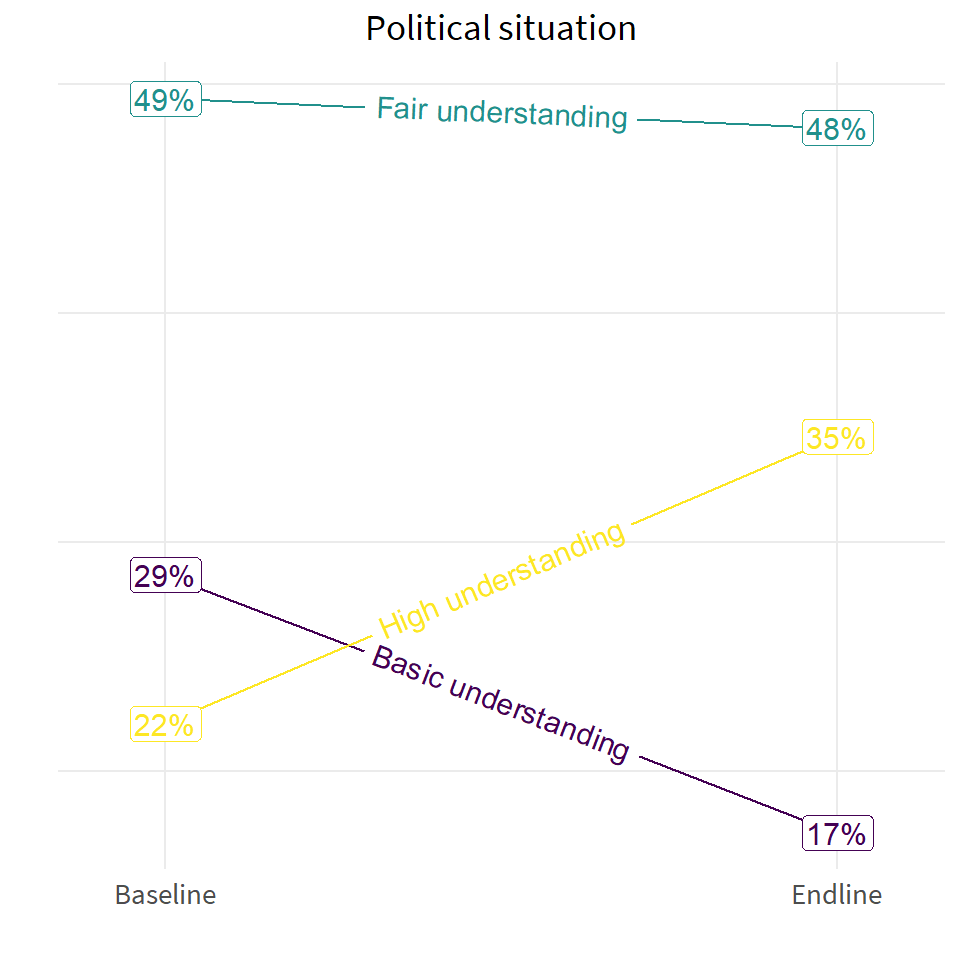
\includegraphics{Data-exploration_files/figure-pdf/unnamed-chunk-2-1.pdf}

\begin{Shaded}
\begin{Highlighting}[]
\NormalTok{soc }\OtherTok{\textless{}{-}} \FunctionTok{ggplot}\NormalTok{(}\FunctionTok{filter}\NormalTok{(df1, item}\SpecialCharTok{==}\StringTok{"Social views"}\NormalTok{), }\FunctionTok{aes}\NormalTok{(endline, perc, }\AttributeTok{color=}\FunctionTok{as.factor}\NormalTok{(response))) }\SpecialCharTok{+} 
  \FunctionTok{geom\_textpath}\NormalTok{(}\FunctionTok{aes}\NormalTok{(}\AttributeTok{label=}\NormalTok{lab),}
                \AttributeTok{size=}\DecValTok{4}\NormalTok{) }\SpecialCharTok{+}
  \FunctionTok{geom\_label}\NormalTok{(}\FunctionTok{aes}\NormalTok{(}\AttributeTok{label=}\FunctionTok{paste}\NormalTok{(}\FunctionTok{round}\NormalTok{(perc}\SpecialCharTok{*}\DecValTok{100}\NormalTok{,}\DecValTok{0}\NormalTok{), }\StringTok{"\%"}\NormalTok{, }\AttributeTok{sep=}\StringTok{""}\NormalTok{)),}
             \AttributeTok{size=}\DecValTok{4}\NormalTok{,}
             \AttributeTok{label.padding =} \FunctionTok{unit}\NormalTok{(.}\DecValTok{14}\NormalTok{, }\StringTok{"lines"}\NormalTok{)) }\SpecialCharTok{+}
  \FunctionTok{scale\_color\_viridis\_d}\NormalTok{(}\AttributeTok{option=}\StringTok{"D"}\NormalTok{) }\SpecialCharTok{+}
  \FunctionTok{scale\_x\_continuous}\NormalTok{(}\AttributeTok{limits=}\FunctionTok{c}\NormalTok{(}\SpecialCharTok{{-}}\NormalTok{.}\DecValTok{1}\NormalTok{, }\FloatTok{1.1}\NormalTok{),}
                     \AttributeTok{breaks=}\FunctionTok{c}\NormalTok{(}\DecValTok{0}\NormalTok{,}\DecValTok{1}\NormalTok{),}
                     \AttributeTok{labels=}\FunctionTok{c}\NormalTok{(}\StringTok{"Baseline"}\NormalTok{,}\StringTok{"Endline"}\NormalTok{)) }\SpecialCharTok{+}
  \FunctionTok{scale\_y\_continuous}\NormalTok{(}\AttributeTok{labels=}\FunctionTok{percent\_format}\NormalTok{(}\AttributeTok{accuracy=}\DecValTok{1}\NormalTok{)) }\SpecialCharTok{+}
  \FunctionTok{theme}\NormalTok{(}\AttributeTok{legend.position=}\StringTok{"none"}\NormalTok{,}
        \AttributeTok{axis.text.y=}\FunctionTok{element\_blank}\NormalTok{()) }\SpecialCharTok{+}
  \FunctionTok{labs}\NormalTok{(}\AttributeTok{x=}\StringTok{""}\NormalTok{,}
       \AttributeTok{y=}\StringTok{""}\NormalTok{,}
       \AttributeTok{title=}\StringTok{"Social situation"}\NormalTok{) }

\NormalTok{soc}
\end{Highlighting}
\end{Shaded}

\begin{verbatim}
Warning in grid.Call(C_textBounds, as.graphicsAnnot(x$label), x$x, x$y, : font
width unknown for character 0x20
\end{verbatim}

\begin{verbatim}
Warning in grid.Call.graphics(C_text, as.graphicsAnnot(x$label), x$x, x$y, :
font width unknown for character 0x20
\end{verbatim}

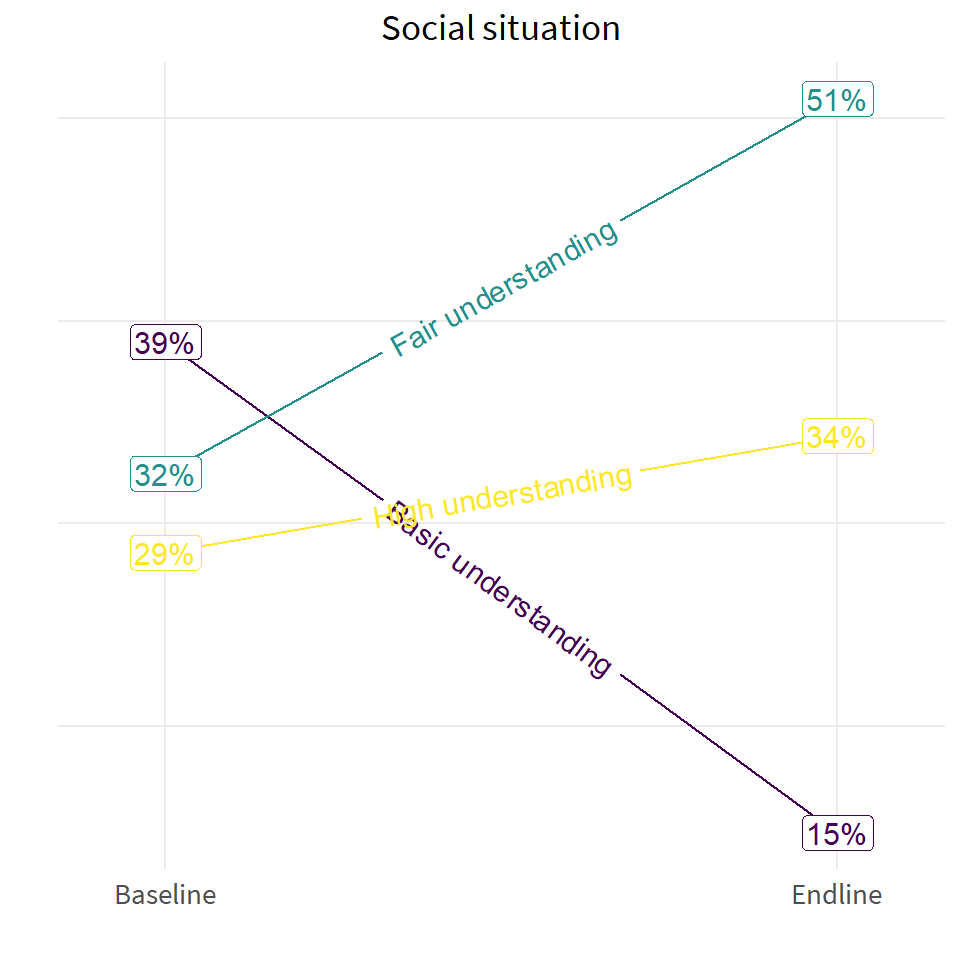
\includegraphics{Data-exploration_files/figure-pdf/unnamed-chunk-3-1.pdf}

\begin{Shaded}
\begin{Highlighting}[]
\NormalTok{ec }\OtherTok{\textless{}{-}} \FunctionTok{ggplot}\NormalTok{(}\FunctionTok{filter}\NormalTok{(df1, item}\SpecialCharTok{==}\StringTok{"Economic views"}\NormalTok{), }\FunctionTok{aes}\NormalTok{(endline, perc, }\AttributeTok{color=}\FunctionTok{as.factor}\NormalTok{(response))) }\SpecialCharTok{+} 
  \FunctionTok{geom\_textpath}\NormalTok{(}\FunctionTok{aes}\NormalTok{(}\AttributeTok{label=}\NormalTok{lab),}
                \AttributeTok{size=}\DecValTok{4}\NormalTok{) }\SpecialCharTok{+}
  \FunctionTok{geom\_label}\NormalTok{(}\FunctionTok{aes}\NormalTok{(}\AttributeTok{label=}\FunctionTok{paste}\NormalTok{(}\FunctionTok{round}\NormalTok{(perc}\SpecialCharTok{*}\DecValTok{100}\NormalTok{,}\DecValTok{0}\NormalTok{), }\StringTok{"\%"}\NormalTok{, }\AttributeTok{sep=}\StringTok{""}\NormalTok{)),}
             \AttributeTok{size=}\DecValTok{4}\NormalTok{,}
             \AttributeTok{label.padding =} \FunctionTok{unit}\NormalTok{(.}\DecValTok{14}\NormalTok{, }\StringTok{"lines"}\NormalTok{)) }\SpecialCharTok{+}
  \FunctionTok{scale\_color\_viridis\_d}\NormalTok{(}\AttributeTok{option=}\StringTok{"D"}\NormalTok{) }\SpecialCharTok{+}
  \FunctionTok{scale\_x\_continuous}\NormalTok{(}\AttributeTok{limits=}\FunctionTok{c}\NormalTok{(}\SpecialCharTok{{-}}\NormalTok{.}\DecValTok{1}\NormalTok{, }\FloatTok{1.1}\NormalTok{),}
                     \AttributeTok{breaks=}\FunctionTok{c}\NormalTok{(}\DecValTok{0}\NormalTok{,}\DecValTok{1}\NormalTok{),}
                     \AttributeTok{labels=}\FunctionTok{c}\NormalTok{(}\StringTok{"Baseline"}\NormalTok{,}\StringTok{"Endline"}\NormalTok{)) }\SpecialCharTok{+}
  \FunctionTok{scale\_y\_continuous}\NormalTok{(}\AttributeTok{labels=}\FunctionTok{percent\_format}\NormalTok{(}\AttributeTok{accuracy=}\DecValTok{1}\NormalTok{)) }\SpecialCharTok{+}
  \FunctionTok{theme}\NormalTok{(}\AttributeTok{legend.position=}\StringTok{"none"}\NormalTok{,}
        \AttributeTok{axis.text.y=}\FunctionTok{element\_blank}\NormalTok{()) }\SpecialCharTok{+}
  \FunctionTok{labs}\NormalTok{(}\AttributeTok{x=}\StringTok{""}\NormalTok{,}
       \AttributeTok{y=}\StringTok{""}\NormalTok{,}
       \AttributeTok{title=}\StringTok{"Economic situation"}\NormalTok{) }

\NormalTok{ec}
\end{Highlighting}
\end{Shaded}

\begin{verbatim}
Warning in grid.Call(C_textBounds, as.graphicsAnnot(x$label), x$x, x$y, : font
width unknown for character 0x20
\end{verbatim}

\begin{verbatim}
Warning in grid.Call.graphics(C_text, as.graphicsAnnot(x$label), x$x, x$y, :
font width unknown for character 0x20
\end{verbatim}

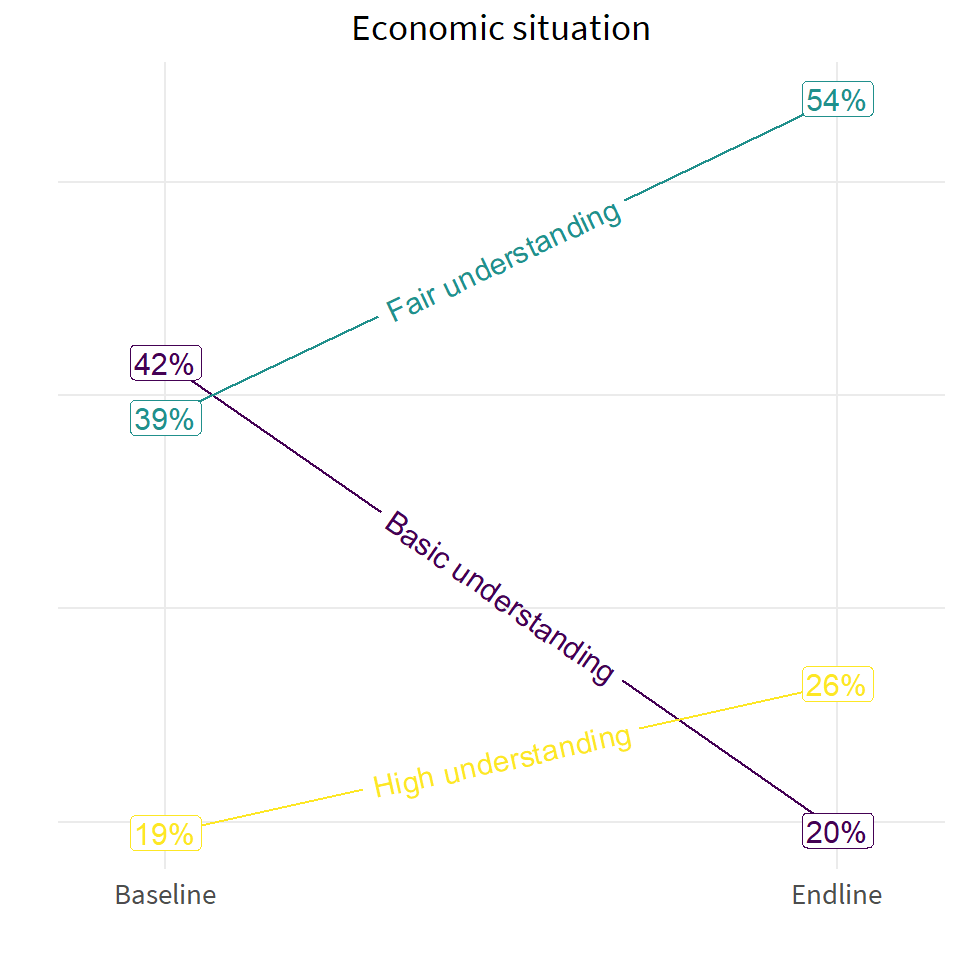
\includegraphics{Data-exploration_files/figure-pdf/unnamed-chunk-4-1.pdf}

Given that the three types of understanding of others' situation are
highly correlated, it makes sense to present these measures compactly as
aspects of a deeper underlying construct. The
\href{https://patchwork.data-imaginist.com/}{patchwork} library allows
multiple ggplots to be assembled together as a single plot. The
following figure illustrates.

\begin{Shaded}
\begin{Highlighting}[]
\NormalTok{pol }\SpecialCharTok{+}\NormalTok{ soc }\SpecialCharTok{+}\NormalTok{ ec }\SpecialCharTok{+} 
  \FunctionTok{plot\_annotation}\NormalTok{(}\AttributeTok{title=}\StringTok{"How well do you understand the situation of others?"}\NormalTok{)}
\end{Highlighting}
\end{Shaded}

\begin{verbatim}
Warning in grid.Call(C_textBounds, as.graphicsAnnot(x$label), x$x, x$y, : font
width unknown for character 0x20
Warning in grid.Call(C_textBounds, as.graphicsAnnot(x$label), x$x, x$y, : font
width unknown for character 0x20
Warning in grid.Call(C_textBounds, as.graphicsAnnot(x$label), x$x, x$y, : font
width unknown for character 0x20
Warning in grid.Call(C_textBounds, as.graphicsAnnot(x$label), x$x, x$y, : font
width unknown for character 0x20
Warning in grid.Call(C_textBounds, as.graphicsAnnot(x$label), x$x, x$y, : font
width unknown for character 0x20
Warning in grid.Call(C_textBounds, as.graphicsAnnot(x$label), x$x, x$y, : font
width unknown for character 0x20
Warning in grid.Call(C_textBounds, as.graphicsAnnot(x$label), x$x, x$y, : font
width unknown for character 0x20
Warning in grid.Call(C_textBounds, as.graphicsAnnot(x$label), x$x, x$y, : font
width unknown for character 0x20
Warning in grid.Call(C_textBounds, as.graphicsAnnot(x$label), x$x, x$y, : font
width unknown for character 0x20
Warning in grid.Call(C_textBounds, as.graphicsAnnot(x$label), x$x, x$y, : font
width unknown for character 0x20
Warning in grid.Call(C_textBounds, as.graphicsAnnot(x$label), x$x, x$y, : font
width unknown for character 0x20
\end{verbatim}

\begin{verbatim}
Warning in grid.Call.graphics(C_text, as.graphicsAnnot(x$label), x$x, x$y, :
font width unknown for character 0x20
Warning in grid.Call.graphics(C_text, as.graphicsAnnot(x$label), x$x, x$y, :
font width unknown for character 0x20
Warning in grid.Call.graphics(C_text, as.graphicsAnnot(x$label), x$x, x$y, :
font width unknown for character 0x20
Warning in grid.Call.graphics(C_text, as.graphicsAnnot(x$label), x$x, x$y, :
font width unknown for character 0x20
Warning in grid.Call.graphics(C_text, as.graphicsAnnot(x$label), x$x, x$y, :
font width unknown for character 0x20
Warning in grid.Call.graphics(C_text, as.graphicsAnnot(x$label), x$x, x$y, :
font width unknown for character 0x20
Warning in grid.Call.graphics(C_text, as.graphicsAnnot(x$label), x$x, x$y, :
font width unknown for character 0x20
Warning in grid.Call.graphics(C_text, as.graphicsAnnot(x$label), x$x, x$y, :
font width unknown for character 0x20
Warning in grid.Call.graphics(C_text, as.graphicsAnnot(x$label), x$x, x$y, :
font width unknown for character 0x20
Warning in grid.Call.graphics(C_text, as.graphicsAnnot(x$label), x$x, x$y, :
font width unknown for character 0x20
Warning in grid.Call.graphics(C_text, as.graphicsAnnot(x$label), x$x, x$y, :
font width unknown for character 0x20
\end{verbatim}

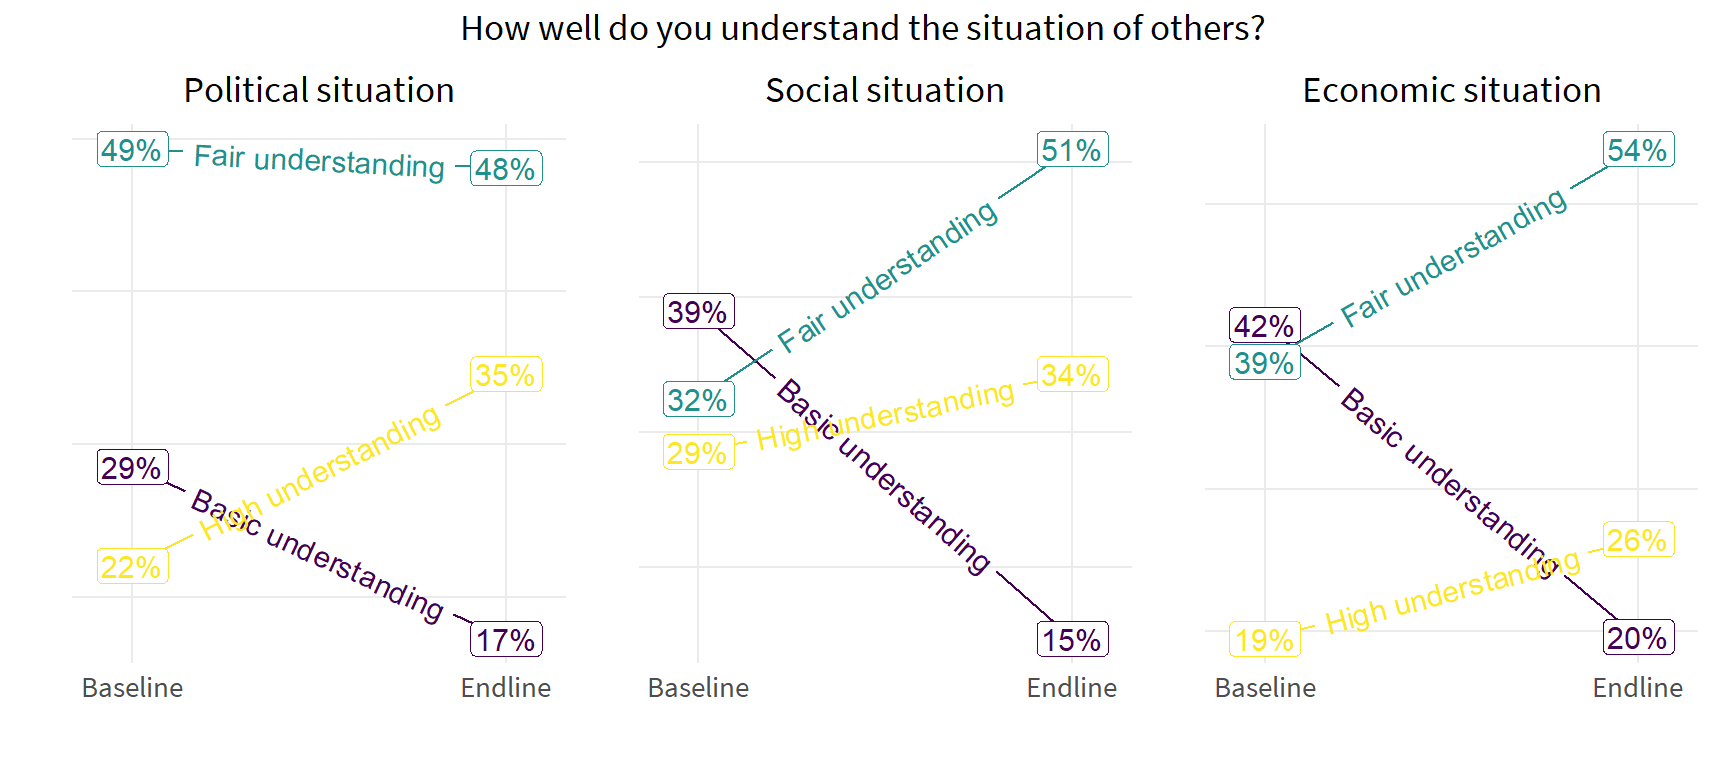
\includegraphics{Data-exploration_files/figure-pdf/unnamed-chunk-5-1.pdf}

A final use of presenting the data more compactly is to collapse the
ordinal responses to binary, and collect the three measures as lines in
a single plot. The following data captures each type of understanding as
either fair or high understanding as one category, and basic
understanding as the other category.

\begin{Shaded}
\begin{Highlighting}[]
\NormalTok{dat }\OtherTok{\textless{}{-}} \FunctionTok{read\_csv}\NormalTok{(}\StringTok{"data/short demo series/meppa item ladder.csv"}\NormalTok{,}
                \AttributeTok{show\_col\_types=}\NormalTok{F)}

\NormalTok{dat\_flx }\OtherTok{\textless{}{-}}\NormalTok{ dat }\SpecialCharTok{\%\textgreater{}\%}
  \FunctionTok{flextable}\NormalTok{() }\SpecialCharTok{\%\textgreater{}\%}
  \FunctionTok{autofit}\NormalTok{() }

\NormalTok{dat\_flx}
\end{Highlighting}
\end{Shaded}

\global\setlength{\Oldarrayrulewidth}{\arrayrulewidth}

\global\setlength{\Oldtabcolsep}{\tabcolsep}

\setlength{\tabcolsep}{2pt}

\renewcommand*{\arraystretch}{1.5}



\providecommand{\ascline}[3]{\noalign{\global\arrayrulewidth #1}\arrayrulecolor[HTML]{#2}\cline{#3}}

\begin{longtable*}[c]{|p{0.78in}|p{0.46in}|p{0.67in}|p{1.57in}}



\ascline{1.5pt}{666666}{1-4}

\multicolumn{1}{>{\raggedleft}m{\dimexpr 0.78in+0\tabcolsep}}{\textcolor[HTML]{000000}{\fontsize{11}{11}\selectfont{\global\setmainfont{Arial}{endline}}}} & \multicolumn{1}{>{\raggedleft}m{\dimexpr 0.46in+0\tabcolsep}}{\textcolor[HTML]{000000}{\fontsize{11}{11}\selectfont{\global\setmainfont{Arial}{n}}}} & \multicolumn{1}{>{\raggedleft}m{\dimexpr 0.67in+0\tabcolsep}}{\textcolor[HTML]{000000}{\fontsize{11}{11}\selectfont{\global\setmainfont{Arial}{perc}}}} & \multicolumn{1}{>{\raggedright}m{\dimexpr 1.57in+0\tabcolsep}}{\textcolor[HTML]{000000}{\fontsize{11}{11}\selectfont{\global\setmainfont{Arial}{item}}}} \\

\ascline{1.5pt}{666666}{1-4}\endfirsthead 

\ascline{1.5pt}{666666}{1-4}

\multicolumn{1}{>{\raggedleft}m{\dimexpr 0.78in+0\tabcolsep}}{\textcolor[HTML]{000000}{\fontsize{11}{11}\selectfont{\global\setmainfont{Arial}{endline}}}} & \multicolumn{1}{>{\raggedleft}m{\dimexpr 0.46in+0\tabcolsep}}{\textcolor[HTML]{000000}{\fontsize{11}{11}\selectfont{\global\setmainfont{Arial}{n}}}} & \multicolumn{1}{>{\raggedleft}m{\dimexpr 0.67in+0\tabcolsep}}{\textcolor[HTML]{000000}{\fontsize{11}{11}\selectfont{\global\setmainfont{Arial}{perc}}}} & \multicolumn{1}{>{\raggedright}m{\dimexpr 1.57in+0\tabcolsep}}{\textcolor[HTML]{000000}{\fontsize{11}{11}\selectfont{\global\setmainfont{Arial}{item}}}} \\

\ascline{1.5pt}{666666}{1-4}\endhead



\multicolumn{1}{>{\raggedleft}m{\dimexpr 0.78in+0\tabcolsep}}{\textcolor[HTML]{000000}{\fontsize{11}{11}\selectfont{\global\setmainfont{Arial}{0}}}} & \multicolumn{1}{>{\raggedleft}m{\dimexpr 0.46in+0\tabcolsep}}{\textcolor[HTML]{000000}{\fontsize{11}{11}\selectfont{\global\setmainfont{Arial}{55}}}} & \multicolumn{1}{>{\raggedleft}m{\dimexpr 0.67in+0\tabcolsep}}{\textcolor[HTML]{000000}{\fontsize{11}{11}\selectfont{\global\setmainfont{Arial}{0.714}}}} & \multicolumn{1}{>{\raggedright}m{\dimexpr 1.57in+0\tabcolsep}}{\textcolor[HTML]{000000}{\fontsize{11}{11}\selectfont{\global\setmainfont{Arial}{Political\ situation}}}} \\





\multicolumn{1}{>{\raggedleft}m{\dimexpr 0.78in+0\tabcolsep}}{\textcolor[HTML]{000000}{\fontsize{11}{11}\selectfont{\global\setmainfont{Arial}{1}}}} & \multicolumn{1}{>{\raggedleft}m{\dimexpr 0.46in+0\tabcolsep}}{\textcolor[HTML]{000000}{\fontsize{11}{11}\selectfont{\global\setmainfont{Arial}{86}}}} & \multicolumn{1}{>{\raggedleft}m{\dimexpr 0.67in+0\tabcolsep}}{\textcolor[HTML]{000000}{\fontsize{11}{11}\selectfont{\global\setmainfont{Arial}{0.827}}}} & \multicolumn{1}{>{\raggedright}m{\dimexpr 1.57in+0\tabcolsep}}{\textcolor[HTML]{000000}{\fontsize{11}{11}\selectfont{\global\setmainfont{Arial}{Political\ situation}}}} \\





\multicolumn{1}{>{\raggedleft}m{\dimexpr 0.78in+0\tabcolsep}}{\textcolor[HTML]{000000}{\fontsize{11}{11}\selectfont{\global\setmainfont{Arial}{0}}}} & \multicolumn{1}{>{\raggedleft}m{\dimexpr 0.46in+0\tabcolsep}}{\textcolor[HTML]{000000}{\fontsize{11}{11}\selectfont{\global\setmainfont{Arial}{47}}}} & \multicolumn{1}{>{\raggedleft}m{\dimexpr 0.67in+0\tabcolsep}}{\textcolor[HTML]{000000}{\fontsize{11}{11}\selectfont{\global\setmainfont{Arial}{0.610}}}} & \multicolumn{1}{>{\raggedright}m{\dimexpr 1.57in+0\tabcolsep}}{\textcolor[HTML]{000000}{\fontsize{11}{11}\selectfont{\global\setmainfont{Arial}{Social\ situation}}}} \\





\multicolumn{1}{>{\raggedleft}m{\dimexpr 0.78in+0\tabcolsep}}{\textcolor[HTML]{000000}{\fontsize{11}{11}\selectfont{\global\setmainfont{Arial}{1}}}} & \multicolumn{1}{>{\raggedleft}m{\dimexpr 0.46in+0\tabcolsep}}{\textcolor[HTML]{000000}{\fontsize{11}{11}\selectfont{\global\setmainfont{Arial}{87}}}} & \multicolumn{1}{>{\raggedleft}m{\dimexpr 0.67in+0\tabcolsep}}{\textcolor[HTML]{000000}{\fontsize{11}{11}\selectfont{\global\setmainfont{Arial}{0.853}}}} & \multicolumn{1}{>{\raggedright}m{\dimexpr 1.57in+0\tabcolsep}}{\textcolor[HTML]{000000}{\fontsize{11}{11}\selectfont{\global\setmainfont{Arial}{Social\ situation}}}} \\





\multicolumn{1}{>{\raggedleft}m{\dimexpr 0.78in+0\tabcolsep}}{\textcolor[HTML]{000000}{\fontsize{11}{11}\selectfont{\global\setmainfont{Arial}{0}}}} & \multicolumn{1}{>{\raggedleft}m{\dimexpr 0.46in+0\tabcolsep}}{\textcolor[HTML]{000000}{\fontsize{11}{11}\selectfont{\global\setmainfont{Arial}{45}}}} & \multicolumn{1}{>{\raggedleft}m{\dimexpr 0.67in+0\tabcolsep}}{\textcolor[HTML]{000000}{\fontsize{11}{11}\selectfont{\global\setmainfont{Arial}{0.584}}}} & \multicolumn{1}{>{\raggedright}m{\dimexpr 1.57in+0\tabcolsep}}{\textcolor[HTML]{000000}{\fontsize{11}{11}\selectfont{\global\setmainfont{Arial}{Economic\ situation}}}} \\





\multicolumn{1}{>{\raggedleft}m{\dimexpr 0.78in+0\tabcolsep}}{\textcolor[HTML]{000000}{\fontsize{11}{11}\selectfont{\global\setmainfont{Arial}{1}}}} & \multicolumn{1}{>{\raggedleft}m{\dimexpr 0.46in+0\tabcolsep}}{\textcolor[HTML]{000000}{\fontsize{11}{11}\selectfont{\global\setmainfont{Arial}{82}}}} & \multicolumn{1}{>{\raggedleft}m{\dimexpr 0.67in+0\tabcolsep}}{\textcolor[HTML]{000000}{\fontsize{11}{11}\selectfont{\global\setmainfont{Arial}{0.804}}}} & \multicolumn{1}{>{\raggedright}m{\dimexpr 1.57in+0\tabcolsep}}{\textcolor[HTML]{000000}{\fontsize{11}{11}\selectfont{\global\setmainfont{Arial}{Economic\ situation}}}} \\

\ascline{1.5pt}{666666}{1-4}



\end{longtable*}



\arrayrulecolor[HTML]{000000}

\global\setlength{\arrayrulewidth}{\Oldarrayrulewidth}

\global\setlength{\tabcolsep}{\Oldtabcolsep}

\renewcommand*{\arraystretch}{1}

With this simplified data summary, the trendline for each type of
understanding may now be collected in a single plot.

\begin{Shaded}
\begin{Highlighting}[]
\FunctionTok{ggplot}\NormalTok{(dat, }\FunctionTok{aes}\NormalTok{(endline, perc, }\AttributeTok{color=}\FunctionTok{as.factor}\NormalTok{(item))) }\SpecialCharTok{+} 
  \FunctionTok{geom\_textpath}\NormalTok{(}\FunctionTok{aes}\NormalTok{(}\AttributeTok{label=}\NormalTok{item),}
                \AttributeTok{size=}\DecValTok{4}\NormalTok{) }\SpecialCharTok{+}
  \FunctionTok{geom\_label}\NormalTok{(}\FunctionTok{aes}\NormalTok{(}\AttributeTok{label=}\FunctionTok{paste}\NormalTok{(}\FunctionTok{round}\NormalTok{(perc}\SpecialCharTok{*}\DecValTok{100}\NormalTok{,}\DecValTok{0}\NormalTok{), }\StringTok{"\%"}\NormalTok{, }\AttributeTok{sep=}\StringTok{""}\NormalTok{)),}
             \AttributeTok{size=}\DecValTok{4}\NormalTok{,}
             \AttributeTok{label.padding =} \FunctionTok{unit}\NormalTok{(.}\DecValTok{14}\NormalTok{, }\StringTok{"lines"}\NormalTok{)) }\SpecialCharTok{+}
  \FunctionTok{scale\_color\_viridis\_d}\NormalTok{(}\AttributeTok{option=}\StringTok{"D"}\NormalTok{) }\SpecialCharTok{+}
  \FunctionTok{scale\_x\_continuous}\NormalTok{(}\AttributeTok{limits=}\FunctionTok{c}\NormalTok{(}\SpecialCharTok{{-}}\NormalTok{.}\DecValTok{1}\NormalTok{, }\FloatTok{1.1}\NormalTok{),}
                     \AttributeTok{breaks=}\FunctionTok{c}\NormalTok{(}\DecValTok{0}\NormalTok{,}\DecValTok{1}\NormalTok{),}
                     \AttributeTok{labels=}\FunctionTok{c}\NormalTok{(}\StringTok{"Baseline"}\NormalTok{,}\StringTok{"Endline"}\NormalTok{)) }\SpecialCharTok{+}
  \FunctionTok{scale\_y\_continuous}\NormalTok{(}\AttributeTok{labels=}\FunctionTok{percent\_format}\NormalTok{(}\AttributeTok{accuracy=}\DecValTok{1}\NormalTok{),}
                     \AttributeTok{breaks=}\FunctionTok{c}\NormalTok{(.}\DecValTok{5}\NormalTok{,}\DecValTok{1}\NormalTok{),}
                     \AttributeTok{sec.axis=}\FunctionTok{dup\_axis}\NormalTok{(}\AttributeTok{breaks=}\FunctionTok{c}\NormalTok{(.}\DecValTok{804}\NormalTok{,.}\DecValTok{827}\NormalTok{,.}\DecValTok{853}\NormalTok{),}
                                       \AttributeTok{labels=}\FunctionTok{c}\NormalTok{(}\StringTok{"+22"}\NormalTok{,}\StringTok{"+12"}\NormalTok{,}\StringTok{"+24"}\NormalTok{))) }\SpecialCharTok{+}
  \FunctionTok{theme}\NormalTok{(}\AttributeTok{legend.position=}\StringTok{"none"}\NormalTok{,}
        \AttributeTok{axis.text.y.left=}\FunctionTok{element\_blank}\NormalTok{()) }\SpecialCharTok{+}
  \FunctionTok{labs}\NormalTok{(}\AttributeTok{x=}\StringTok{""}\NormalTok{,}
       \AttributeTok{y=}\StringTok{""}\NormalTok{,}
       \AttributeTok{caption=}\StringTok{"Proportion reporting fair or high}\SpecialCharTok{\textbackslash{}n}\StringTok{understanding of others\textquotesingle{} situation"}\NormalTok{)}
\end{Highlighting}
\end{Shaded}

\begin{verbatim}
Warning in grid.Call(C_textBounds, as.graphicsAnnot(x$label), x$x, x$y, : font
width unknown for character 0x20
Warning in grid.Call(C_textBounds, as.graphicsAnnot(x$label), x$x, x$y, : font
width unknown for character 0x20
Warning in grid.Call(C_textBounds, as.graphicsAnnot(x$label), x$x, x$y, : font
width unknown for character 0x20
Warning in grid.Call(C_textBounds, as.graphicsAnnot(x$label), x$x, x$y, : font
width unknown for character 0x20
Warning in grid.Call(C_textBounds, as.graphicsAnnot(x$label), x$x, x$y, : font
width unknown for character 0x20
Warning in grid.Call(C_textBounds, as.graphicsAnnot(x$label), x$x, x$y, : font
width unknown for character 0x20
Warning in grid.Call(C_textBounds, as.graphicsAnnot(x$label), x$x, x$y, : font
width unknown for character 0x20
\end{verbatim}

\begin{verbatim}
Warning in grid.Call.graphics(C_text, as.graphicsAnnot(x$label), x$x, x$y, :
font width unknown for character 0x20
Warning in grid.Call.graphics(C_text, as.graphicsAnnot(x$label), x$x, x$y, :
font width unknown for character 0x20
Warning in grid.Call.graphics(C_text, as.graphicsAnnot(x$label), x$x, x$y, :
font width unknown for character 0x20
Warning in grid.Call.graphics(C_text, as.graphicsAnnot(x$label), x$x, x$y, :
font width unknown for character 0x20
Warning in grid.Call.graphics(C_text, as.graphicsAnnot(x$label), x$x, x$y, :
font width unknown for character 0x20
Warning in grid.Call.graphics(C_text, as.graphicsAnnot(x$label), x$x, x$y, :
font width unknown for character 0x20
Warning in grid.Call.graphics(C_text, as.graphicsAnnot(x$label), x$x, x$y, :
font width unknown for character 0x20
\end{verbatim}

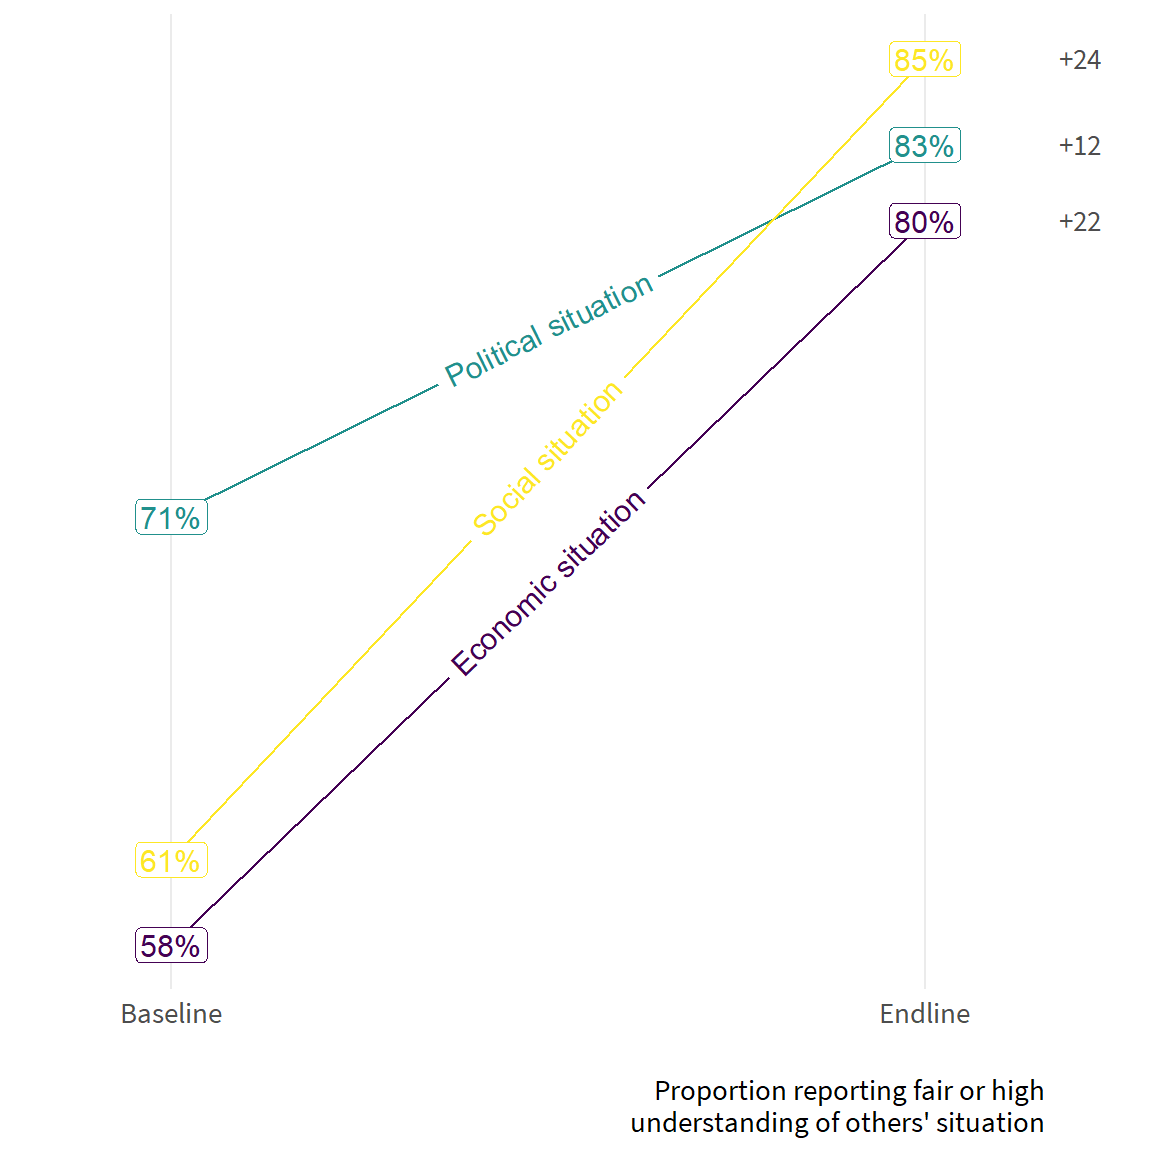
\includegraphics{Data-exploration_files/figure-pdf/unnamed-chunk-7-1.pdf}

Note further the use of secondary axis breaks to illustrate the change
score for each trendline from baseline to endline.

The R computing language allows for several ways to customize the use of
labels in statistical or descriptive graphics. This short demo has
illustrated MSI's use of the geomtextpath package to place labels
directly along the line or curve of a plot. This illustration used only
straight lines between two points in time. For additional use cases of
the geomtextpath package, see the package
\href{https://cran.r-project.org/web/packages/geomtextpath/vignettes/geomtextpath.html}{vignette}.

\subsection{Gantt charts}\label{gantt-charts}

Sometimes it can be helpful to incorporate a more visual presentation of
Gantt charts into our planning documents and client communications. The
following table is an example of a simplified Gantt that was extracted
from a larger Gantt from for the purposes of identifying the specific
areas that could be subject to monitoring or evaluation activities.

\begin{Shaded}
\begin{Highlighting}[]
\NormalTok{gantt }\OtherTok{\textless{}{-}} \FunctionTok{read\_excel}\NormalTok{(}\StringTok{"data/short demo series/aqbe {-} GANTT.xlsx"}\NormalTok{)}

\NormalTok{gantt }\SpecialCharTok{\%\textgreater{}\%}
  \FunctionTok{flextable}\NormalTok{()}
\end{Highlighting}
\end{Shaded}

\global\setlength{\Oldarrayrulewidth}{\arrayrulewidth}

\global\setlength{\Oldtabcolsep}{\tabcolsep}

\setlength{\tabcolsep}{2pt}

\renewcommand*{\arraystretch}{1.5}



\providecommand{\ascline}[3]{\noalign{\global\arrayrulewidth #1}\arrayrulecolor[HTML]{#2}\cline{#3}}

\begin{longtable*}[c]{|p{0.75in}|p{0.75in}|p{0.75in}|p{0.75in}|p{0.75in}|p{0.75in}|p{0.75in}|p{0.75in}|p{0.75in}|p{0.75in}|p{0.75in}}



\ascline{1.5pt}{666666}{1-11}

\multicolumn{1}{>{\raggedleft}m{\dimexpr 0.75in+0\tabcolsep}}{\textcolor[HTML]{000000}{\fontsize{11}{11}\selectfont{\global\setmainfont{Arial}{num}}}} & \multicolumn{1}{>{\raggedright}m{\dimexpr 0.75in+0\tabcolsep}}{\textcolor[HTML]{000000}{\fontsize{11}{11}\selectfont{\global\setmainfont{Arial}{act}}}} & \multicolumn{1}{>{\raggedright}m{\dimexpr 0.75in+0\tabcolsep}}{\textcolor[HTML]{000000}{\fontsize{11}{11}\selectfont{\global\setmainfont{Arial}{Activity}}}} & \multicolumn{1}{>{\raggedleft}m{\dimexpr 0.75in+0\tabcolsep}}{\textcolor[HTML]{000000}{\fontsize{11}{11}\selectfont{\global\setmainfont{Arial}{Cohort}}}} & \multicolumn{1}{>{\raggedright}m{\dimexpr 0.75in+0\tabcolsep}}{\textcolor[HTML]{000000}{\fontsize{11}{11}\selectfont{\global\setmainfont{Arial}{Climate\ zone}}}} & \multicolumn{1}{>{\raggedright}m{\dimexpr 0.75in+0\tabcolsep}}{\textcolor[HTML]{000000}{\fontsize{11}{11}\selectfont{\global\setmainfont{Arial}{Label}}}} & \multicolumn{1}{>{\raggedright}m{\dimexpr 0.75in+0\tabcolsep}}{\textcolor[HTML]{000000}{\fontsize{11}{11}\selectfont{\global\setmainfont{Arial}{Label2}}}} & \multicolumn{1}{>{\raggedright}m{\dimexpr 0.75in+0\tabcolsep}}{\textcolor[HTML]{000000}{\fontsize{11}{11}\selectfont{\global\setmainfont{Arial}{Label3}}}} & \multicolumn{1}{>{\raggedright}m{\dimexpr 0.75in+0\tabcolsep}}{\textcolor[HTML]{000000}{\fontsize{11}{11}\selectfont{\global\setmainfont{Arial}{Label4}}}} & \multicolumn{1}{>{\raggedleft}m{\dimexpr 0.75in+0\tabcolsep}}{\textcolor[HTML]{000000}{\fontsize{11}{11}\selectfont{\global\setmainfont{Arial}{Start}}}} & \multicolumn{1}{>{\raggedleft}m{\dimexpr 0.75in+0\tabcolsep}}{\textcolor[HTML]{000000}{\fontsize{11}{11}\selectfont{\global\setmainfont{Arial}{Finish}}}} \\

\ascline{1.5pt}{666666}{1-11}\endfirsthead 

\ascline{1.5pt}{666666}{1-11}

\multicolumn{1}{>{\raggedleft}m{\dimexpr 0.75in+0\tabcolsep}}{\textcolor[HTML]{000000}{\fontsize{11}{11}\selectfont{\global\setmainfont{Arial}{num}}}} & \multicolumn{1}{>{\raggedright}m{\dimexpr 0.75in+0\tabcolsep}}{\textcolor[HTML]{000000}{\fontsize{11}{11}\selectfont{\global\setmainfont{Arial}{act}}}} & \multicolumn{1}{>{\raggedright}m{\dimexpr 0.75in+0\tabcolsep}}{\textcolor[HTML]{000000}{\fontsize{11}{11}\selectfont{\global\setmainfont{Arial}{Activity}}}} & \multicolumn{1}{>{\raggedleft}m{\dimexpr 0.75in+0\tabcolsep}}{\textcolor[HTML]{000000}{\fontsize{11}{11}\selectfont{\global\setmainfont{Arial}{Cohort}}}} & \multicolumn{1}{>{\raggedright}m{\dimexpr 0.75in+0\tabcolsep}}{\textcolor[HTML]{000000}{\fontsize{11}{11}\selectfont{\global\setmainfont{Arial}{Climate\ zone}}}} & \multicolumn{1}{>{\raggedright}m{\dimexpr 0.75in+0\tabcolsep}}{\textcolor[HTML]{000000}{\fontsize{11}{11}\selectfont{\global\setmainfont{Arial}{Label}}}} & \multicolumn{1}{>{\raggedright}m{\dimexpr 0.75in+0\tabcolsep}}{\textcolor[HTML]{000000}{\fontsize{11}{11}\selectfont{\global\setmainfont{Arial}{Label2}}}} & \multicolumn{1}{>{\raggedright}m{\dimexpr 0.75in+0\tabcolsep}}{\textcolor[HTML]{000000}{\fontsize{11}{11}\selectfont{\global\setmainfont{Arial}{Label3}}}} & \multicolumn{1}{>{\raggedright}m{\dimexpr 0.75in+0\tabcolsep}}{\textcolor[HTML]{000000}{\fontsize{11}{11}\selectfont{\global\setmainfont{Arial}{Label4}}}} & \multicolumn{1}{>{\raggedleft}m{\dimexpr 0.75in+0\tabcolsep}}{\textcolor[HTML]{000000}{\fontsize{11}{11}\selectfont{\global\setmainfont{Arial}{Start}}}} & \multicolumn{1}{>{\raggedleft}m{\dimexpr 0.75in+0\tabcolsep}}{\textcolor[HTML]{000000}{\fontsize{11}{11}\selectfont{\global\setmainfont{Arial}{Finish}}}} \\

\ascline{1.5pt}{666666}{1-11}\endhead



\multicolumn{1}{>{\raggedleft}m{\dimexpr 0.75in+0\tabcolsep}}{\textcolor[HTML]{000000}{\fontsize{11}{11}\selectfont{\global\setmainfont{Arial}{1}}}} & \multicolumn{1}{>{\raggedright}m{\dimexpr 0.75in+0\tabcolsep}}{\textcolor[HTML]{000000}{\fontsize{11}{11}\selectfont{\global\setmainfont{Arial}{1.1.2}}}} & \multicolumn{1}{>{\raggedright}m{\dimexpr 0.75in+0\tabcolsep}}{\textcolor[HTML]{000000}{\fontsize{11}{11}\selectfont{\global\setmainfont{Arial}{Professional\ development\ instruments\ and\ models}}}} & \multicolumn{1}{>{\raggedleft}m{\dimexpr 0.75in+0\tabcolsep}}{\textcolor[HTML]{000000}{\fontsize{11}{11}\selectfont{\global\setmainfont{Arial}{}}}} & \multicolumn{1}{>{\raggedright}m{\dimexpr 0.75in+0\tabcolsep}}{\textcolor[HTML]{000000}{\fontsize{11}{11}\selectfont{\global\setmainfont{Arial}{}}}} & \multicolumn{1}{>{\raggedright}m{\dimexpr 0.75in+0\tabcolsep}}{\textcolor[HTML]{000000}{\fontsize{11}{11}\selectfont{\global\setmainfont{Arial}{35\ Master\ Trainers\ and\ 7\ Teacher\ Educators\ trained}}}} & \multicolumn{1}{>{\raggedright}m{\dimexpr 0.75in+0\tabcolsep}}{\textcolor[HTML]{000000}{\fontsize{11}{11}\selectfont{\global\setmainfont{Arial}{35\ Master\ Trainers\ and\ 7\ Teacher\ Educators\ trained}}}} & \multicolumn{1}{>{\raggedright}m{\dimexpr 0.75in+0\tabcolsep}}{\textcolor[HTML]{000000}{\fontsize{11}{11}\selectfont{\global\setmainfont{Arial}{35\ Master\ Trainers}}}} & \multicolumn{1}{>{\raggedright}m{\dimexpr 0.75in+0\tabcolsep}}{\textcolor[HTML]{000000}{\fontsize{11}{11}\selectfont{\global\setmainfont{Arial}{35}}}} & \multicolumn{1}{>{\raggedleft}m{\dimexpr 0.75in+0\tabcolsep}}{\textcolor[HTML]{000000}{\fontsize{11}{11}\selectfont{\global\setmainfont{Arial}{2024-11-01\ 00:00:00}}}} & \multicolumn{1}{>{\raggedleft}m{\dimexpr 0.75in+0\tabcolsep}}{\textcolor[HTML]{000000}{\fontsize{11}{11}\selectfont{\global\setmainfont{Arial}{2025-01-01\ 00:00:00}}}} \\





\multicolumn{1}{>{\raggedleft}m{\dimexpr 0.75in+0\tabcolsep}}{\textcolor[HTML]{000000}{\fontsize{11}{11}\selectfont{\global\setmainfont{Arial}{2}}}} & \multicolumn{1}{>{\raggedright}m{\dimexpr 0.75in+0\tabcolsep}}{\textcolor[HTML]{000000}{\fontsize{11}{11}\selectfont{\global\setmainfont{Arial}{1.1.4}}}} & \multicolumn{1}{>{\raggedright}m{\dimexpr 0.75in+0\tabcolsep}}{\textcolor[HTML]{000000}{\fontsize{11}{11}\selectfont{\global\setmainfont{Arial}{Teachers\ trained\ on\ UNICEF\ Package}}}} & \multicolumn{1}{>{\raggedleft}m{\dimexpr 0.75in+0\tabcolsep}}{\textcolor[HTML]{000000}{\fontsize{11}{11}\selectfont{\global\setmainfont{Arial}{1}}}} & \multicolumn{1}{>{\raggedright}m{\dimexpr 0.75in+0\tabcolsep}}{\textcolor[HTML]{000000}{\fontsize{11}{11}\selectfont{\global\setmainfont{Arial}{Warm}}}} & \multicolumn{1}{>{\raggedright}m{\dimexpr 0.75in+0\tabcolsep}}{\textcolor[HTML]{000000}{\fontsize{11}{11}\selectfont{\global\setmainfont{Arial}{Cohort\ 1,\ Year\ 1,\ Warm\ Climate}}}} & \multicolumn{1}{>{\raggedright}m{\dimexpr 0.75in+0\tabcolsep}}{\textcolor[HTML]{000000}{\fontsize{11}{11}\selectfont{\global\setmainfont{Arial}{400\ CBE\ /\ 2,625\ teachers\ trained}}}} & \multicolumn{1}{>{\raggedright}m{\dimexpr 0.75in+0\tabcolsep}}{\textcolor[HTML]{000000}{\fontsize{11}{11}\selectfont{\global\setmainfont{Arial}{400\ CBE\ /\ 2,625\ teachers}}}} & \multicolumn{1}{>{\raggedright}m{\dimexpr 0.75in+0\tabcolsep}}{\textcolor[HTML]{000000}{\fontsize{11}{11}\selectfont{\global\setmainfont{Arial}{3025}}}} & \multicolumn{1}{>{\raggedleft}m{\dimexpr 0.75in+0\tabcolsep}}{\textcolor[HTML]{000000}{\fontsize{11}{11}\selectfont{\global\setmainfont{Arial}{2024-05-01\ 00:00:00}}}} & \multicolumn{1}{>{\raggedleft}m{\dimexpr 0.75in+0\tabcolsep}}{\textcolor[HTML]{000000}{\fontsize{11}{11}\selectfont{\global\setmainfont{Arial}{2024-09-01\ 00:00:00}}}} \\





\multicolumn{1}{>{\raggedleft}m{\dimexpr 0.75in+0\tabcolsep}}{\textcolor[HTML]{000000}{\fontsize{11}{11}\selectfont{\global\setmainfont{Arial}{3}}}} & \multicolumn{1}{>{\raggedright}m{\dimexpr 0.75in+0\tabcolsep}}{\textcolor[HTML]{000000}{\fontsize{11}{11}\selectfont{\global\setmainfont{Arial}{1.1.4}}}} & \multicolumn{1}{>{\raggedright}m{\dimexpr 0.75in+0\tabcolsep}}{\textcolor[HTML]{000000}{\fontsize{11}{11}\selectfont{\global\setmainfont{Arial}{Teachers\ trained\ on\ UNICEF\ Package}}}} & \multicolumn{1}{>{\raggedleft}m{\dimexpr 0.75in+0\tabcolsep}}{\textcolor[HTML]{000000}{\fontsize{11}{11}\selectfont{\global\setmainfont{Arial}{1}}}} & \multicolumn{1}{>{\raggedright}m{\dimexpr 0.75in+0\tabcolsep}}{\textcolor[HTML]{000000}{\fontsize{11}{11}\selectfont{\global\setmainfont{Arial}{Cold}}}} & \multicolumn{1}{>{\raggedright}m{\dimexpr 0.75in+0\tabcolsep}}{\textcolor[HTML]{000000}{\fontsize{11}{11}\selectfont{\global\setmainfont{Arial}{Cohort\ 1,\ Year\ 2,\ Cold\ Climate}}}} & \multicolumn{1}{>{\raggedright}m{\dimexpr 0.75in+0\tabcolsep}}{\textcolor[HTML]{000000}{\fontsize{11}{11}\selectfont{\global\setmainfont{Arial}{400\ CBE\ /\ 2,625\ teachers\ trained}}}} & \multicolumn{1}{>{\raggedright}m{\dimexpr 0.75in+0\tabcolsep}}{\textcolor[HTML]{000000}{\fontsize{11}{11}\selectfont{\global\setmainfont{Arial}{400\ CBE\ /\ 2,625\ teachers}}}} & \multicolumn{1}{>{\raggedright}m{\dimexpr 0.75in+0\tabcolsep}}{\textcolor[HTML]{000000}{\fontsize{11}{11}\selectfont{\global\setmainfont{Arial}{3025}}}} & \multicolumn{1}{>{\raggedleft}m{\dimexpr 0.75in+0\tabcolsep}}{\textcolor[HTML]{000000}{\fontsize{11}{11}\selectfont{\global\setmainfont{Arial}{2024-12-01\ 00:00:00}}}} & \multicolumn{1}{>{\raggedleft}m{\dimexpr 0.75in+0\tabcolsep}}{\textcolor[HTML]{000000}{\fontsize{11}{11}\selectfont{\global\setmainfont{Arial}{2025-04-01\ 00:00:00}}}} \\





\multicolumn{1}{>{\raggedleft}m{\dimexpr 0.75in+0\tabcolsep}}{\textcolor[HTML]{000000}{\fontsize{11}{11}\selectfont{\global\setmainfont{Arial}{4}}}} & \multicolumn{1}{>{\raggedright}m{\dimexpr 0.75in+0\tabcolsep}}{\textcolor[HTML]{000000}{\fontsize{11}{11}\selectfont{\global\setmainfont{Arial}{1.1.4}}}} & \multicolumn{1}{>{\raggedright}m{\dimexpr 0.75in+0\tabcolsep}}{\textcolor[HTML]{000000}{\fontsize{11}{11}\selectfont{\global\setmainfont{Arial}{Teachers\ trained\ on\ UNICEF\ Package}}}} & \multicolumn{1}{>{\raggedleft}m{\dimexpr 0.75in+0\tabcolsep}}{\textcolor[HTML]{000000}{\fontsize{11}{11}\selectfont{\global\setmainfont{Arial}{2}}}} & \multicolumn{1}{>{\raggedright}m{\dimexpr 0.75in+0\tabcolsep}}{\textcolor[HTML]{000000}{\fontsize{11}{11}\selectfont{\global\setmainfont{Arial}{Warm}}}} & \multicolumn{1}{>{\raggedright}m{\dimexpr 0.75in+0\tabcolsep}}{\textcolor[HTML]{000000}{\fontsize{11}{11}\selectfont{\global\setmainfont{Arial}{Cohort\ 2,\ Year\ 3,\ Warm\ Climate}}}} & \multicolumn{1}{>{\raggedright}m{\dimexpr 0.75in+0\tabcolsep}}{\textcolor[HTML]{000000}{\fontsize{11}{11}\selectfont{\global\setmainfont{Arial}{400\ CBE\ /\ 2,625\ teachers\ trained}}}} & \multicolumn{1}{>{\raggedright}m{\dimexpr 0.75in+0\tabcolsep}}{\textcolor[HTML]{000000}{\fontsize{11}{11}\selectfont{\global\setmainfont{Arial}{400\ CBE\ /\ 2,625\ teachers}}}} & \multicolumn{1}{>{\raggedright}m{\dimexpr 0.75in+0\tabcolsep}}{\textcolor[HTML]{000000}{\fontsize{11}{11}\selectfont{\global\setmainfont{Arial}{3025}}}} & \multicolumn{1}{>{\raggedleft}m{\dimexpr 0.75in+0\tabcolsep}}{\textcolor[HTML]{000000}{\fontsize{11}{11}\selectfont{\global\setmainfont{Arial}{2026-05-01\ 00:00:00}}}} & \multicolumn{1}{>{\raggedleft}m{\dimexpr 0.75in+0\tabcolsep}}{\textcolor[HTML]{000000}{\fontsize{11}{11}\selectfont{\global\setmainfont{Arial}{2026-09-01\ 00:00:00}}}} \\





\multicolumn{1}{>{\raggedleft}m{\dimexpr 0.75in+0\tabcolsep}}{\textcolor[HTML]{000000}{\fontsize{11}{11}\selectfont{\global\setmainfont{Arial}{5}}}} & \multicolumn{1}{>{\raggedright}m{\dimexpr 0.75in+0\tabcolsep}}{\textcolor[HTML]{000000}{\fontsize{11}{11}\selectfont{\global\setmainfont{Arial}{1.1.4}}}} & \multicolumn{1}{>{\raggedright}m{\dimexpr 0.75in+0\tabcolsep}}{\textcolor[HTML]{000000}{\fontsize{11}{11}\selectfont{\global\setmainfont{Arial}{Teachers\ trained\ on\ UNICEF\ Package}}}} & \multicolumn{1}{>{\raggedleft}m{\dimexpr 0.75in+0\tabcolsep}}{\textcolor[HTML]{000000}{\fontsize{11}{11}\selectfont{\global\setmainfont{Arial}{2}}}} & \multicolumn{1}{>{\raggedright}m{\dimexpr 0.75in+0\tabcolsep}}{\textcolor[HTML]{000000}{\fontsize{11}{11}\selectfont{\global\setmainfont{Arial}{Cold}}}} & \multicolumn{1}{>{\raggedright}m{\dimexpr 0.75in+0\tabcolsep}}{\textcolor[HTML]{000000}{\fontsize{11}{11}\selectfont{\global\setmainfont{Arial}{Cohort\ 2,\ Year\ 4,\ Cold\ Climate}}}} & \multicolumn{1}{>{\raggedright}m{\dimexpr 0.75in+0\tabcolsep}}{\textcolor[HTML]{000000}{\fontsize{11}{11}\selectfont{\global\setmainfont{Arial}{400\ CBE\ /\ 2,625\ teachers\ trained}}}} & \multicolumn{1}{>{\raggedright}m{\dimexpr 0.75in+0\tabcolsep}}{\textcolor[HTML]{000000}{\fontsize{11}{11}\selectfont{\global\setmainfont{Arial}{400\ CBE\ /\ 2,625\ teachers}}}} & \multicolumn{1}{>{\raggedright}m{\dimexpr 0.75in+0\tabcolsep}}{\textcolor[HTML]{000000}{\fontsize{11}{11}\selectfont{\global\setmainfont{Arial}{3025}}}} & \multicolumn{1}{>{\raggedleft}m{\dimexpr 0.75in+0\tabcolsep}}{\textcolor[HTML]{000000}{\fontsize{11}{11}\selectfont{\global\setmainfont{Arial}{2026-12-01\ 00:00:00}}}} & \multicolumn{1}{>{\raggedleft}m{\dimexpr 0.75in+0\tabcolsep}}{\textcolor[HTML]{000000}{\fontsize{11}{11}\selectfont{\global\setmainfont{Arial}{2027-04-01\ 00:00:00}}}} \\





\multicolumn{1}{>{\raggedleft}m{\dimexpr 0.75in+0\tabcolsep}}{\textcolor[HTML]{000000}{\fontsize{11}{11}\selectfont{\global\setmainfont{Arial}{6}}}} & \multicolumn{1}{>{\raggedright}m{\dimexpr 0.75in+0\tabcolsep}}{\textcolor[HTML]{000000}{\fontsize{11}{11}\selectfont{\global\setmainfont{Arial}{1.1.8}}}} & \multicolumn{1}{>{\raggedright}m{\dimexpr 0.75in+0\tabcolsep}}{\textcolor[HTML]{000000}{\fontsize{11}{11}\selectfont{\global\setmainfont{Arial}{Teacher-learner\ materials}}}} & \multicolumn{1}{>{\raggedleft}m{\dimexpr 0.75in+0\tabcolsep}}{\textcolor[HTML]{000000}{\fontsize{11}{11}\selectfont{\global\setmainfont{Arial}{1}}}} & \multicolumn{1}{>{\raggedright}m{\dimexpr 0.75in+0\tabcolsep}}{\textcolor[HTML]{000000}{\fontsize{11}{11}\selectfont{\global\setmainfont{Arial}{Warm}}}} & \multicolumn{1}{>{\raggedright}m{\dimexpr 0.75in+0\tabcolsep}}{\textcolor[HTML]{000000}{\fontsize{11}{11}\selectfont{\global\setmainfont{Arial}{Cohort\ 1,\ Year\ 1,\ Warm\ Climate}}}} & \multicolumn{1}{>{\raggedright}m{\dimexpr 0.75in+0\tabcolsep}}{\textcolor[HTML]{000000}{\fontsize{11}{11}\selectfont{\global\setmainfont{Arial}{2,625\ teachers\ /\ 52,500\ students}}}} & \multicolumn{1}{>{\raggedright}m{\dimexpr 0.75in+0\tabcolsep}}{\textcolor[HTML]{000000}{\fontsize{11}{11}\selectfont{\global\setmainfont{Arial}{2,625\ teachers\ /\ 52,500\ students}}}} & \multicolumn{1}{>{\raggedright}m{\dimexpr 0.75in+0\tabcolsep}}{\textcolor[HTML]{000000}{\fontsize{11}{11}\selectfont{\global\setmainfont{Arial}{2,625\ T\ /\ 52,500\ S}}}} & \multicolumn{1}{>{\raggedleft}m{\dimexpr 0.75in+0\tabcolsep}}{\textcolor[HTML]{000000}{\fontsize{11}{11}\selectfont{\global\setmainfont{Arial}{2024-05-01\ 00:00:00}}}} & \multicolumn{1}{>{\raggedleft}m{\dimexpr 0.75in+0\tabcolsep}}{\textcolor[HTML]{000000}{\fontsize{11}{11}\selectfont{\global\setmainfont{Arial}{2024-09-01\ 00:00:00}}}} \\





\multicolumn{1}{>{\raggedleft}m{\dimexpr 0.75in+0\tabcolsep}}{\textcolor[HTML]{000000}{\fontsize{11}{11}\selectfont{\global\setmainfont{Arial}{7}}}} & \multicolumn{1}{>{\raggedright}m{\dimexpr 0.75in+0\tabcolsep}}{\textcolor[HTML]{000000}{\fontsize{11}{11}\selectfont{\global\setmainfont{Arial}{1.1.8}}}} & \multicolumn{1}{>{\raggedright}m{\dimexpr 0.75in+0\tabcolsep}}{\textcolor[HTML]{000000}{\fontsize{11}{11}\selectfont{\global\setmainfont{Arial}{Teacher-learner\ materials}}}} & \multicolumn{1}{>{\raggedleft}m{\dimexpr 0.75in+0\tabcolsep}}{\textcolor[HTML]{000000}{\fontsize{11}{11}\selectfont{\global\setmainfont{Arial}{1}}}} & \multicolumn{1}{>{\raggedright}m{\dimexpr 0.75in+0\tabcolsep}}{\textcolor[HTML]{000000}{\fontsize{11}{11}\selectfont{\global\setmainfont{Arial}{Cold}}}} & \multicolumn{1}{>{\raggedright}m{\dimexpr 0.75in+0\tabcolsep}}{\textcolor[HTML]{000000}{\fontsize{11}{11}\selectfont{\global\setmainfont{Arial}{Cohort\ 1,\ Year\ 2,\ Cold\ Climate}}}} & \multicolumn{1}{>{\raggedright}m{\dimexpr 0.75in+0\tabcolsep}}{\textcolor[HTML]{000000}{\fontsize{11}{11}\selectfont{\global\setmainfont{Arial}{2,625\ teachers\ /\ 52,500\ students}}}} & \multicolumn{1}{>{\raggedright}m{\dimexpr 0.75in+0\tabcolsep}}{\textcolor[HTML]{000000}{\fontsize{11}{11}\selectfont{\global\setmainfont{Arial}{2,625\ teachers\ /\ 52,500\ students}}}} & \multicolumn{1}{>{\raggedright}m{\dimexpr 0.75in+0\tabcolsep}}{\textcolor[HTML]{000000}{\fontsize{11}{11}\selectfont{\global\setmainfont{Arial}{2,625\ T\ /\ 52,500\ S}}}} & \multicolumn{1}{>{\raggedleft}m{\dimexpr 0.75in+0\tabcolsep}}{\textcolor[HTML]{000000}{\fontsize{11}{11}\selectfont{\global\setmainfont{Arial}{2024-12-01\ 00:00:00}}}} & \multicolumn{1}{>{\raggedleft}m{\dimexpr 0.75in+0\tabcolsep}}{\textcolor[HTML]{000000}{\fontsize{11}{11}\selectfont{\global\setmainfont{Arial}{2025-04-01\ 00:00:00}}}} \\





\multicolumn{1}{>{\raggedleft}m{\dimexpr 0.75in+0\tabcolsep}}{\textcolor[HTML]{000000}{\fontsize{11}{11}\selectfont{\global\setmainfont{Arial}{8}}}} & \multicolumn{1}{>{\raggedright}m{\dimexpr 0.75in+0\tabcolsep}}{\textcolor[HTML]{000000}{\fontsize{11}{11}\selectfont{\global\setmainfont{Arial}{1.1.8}}}} & \multicolumn{1}{>{\raggedright}m{\dimexpr 0.75in+0\tabcolsep}}{\textcolor[HTML]{000000}{\fontsize{11}{11}\selectfont{\global\setmainfont{Arial}{Teacher-learner\ materials}}}} & \multicolumn{1}{>{\raggedleft}m{\dimexpr 0.75in+0\tabcolsep}}{\textcolor[HTML]{000000}{\fontsize{11}{11}\selectfont{\global\setmainfont{Arial}{2}}}} & \multicolumn{1}{>{\raggedright}m{\dimexpr 0.75in+0\tabcolsep}}{\textcolor[HTML]{000000}{\fontsize{11}{11}\selectfont{\global\setmainfont{Arial}{Warm}}}} & \multicolumn{1}{>{\raggedright}m{\dimexpr 0.75in+0\tabcolsep}}{\textcolor[HTML]{000000}{\fontsize{11}{11}\selectfont{\global\setmainfont{Arial}{Cohort\ 2,\ Year\ 3,\ Warm\ Climate}}}} & \multicolumn{1}{>{\raggedright}m{\dimexpr 0.75in+0\tabcolsep}}{\textcolor[HTML]{000000}{\fontsize{11}{11}\selectfont{\global\setmainfont{Arial}{2,625\ teachers\ /\ 52,500\ students}}}} & \multicolumn{1}{>{\raggedright}m{\dimexpr 0.75in+0\tabcolsep}}{\textcolor[HTML]{000000}{\fontsize{11}{11}\selectfont{\global\setmainfont{Arial}{2,625\ teachers\ /\ 52,500\ students}}}} & \multicolumn{1}{>{\raggedright}m{\dimexpr 0.75in+0\tabcolsep}}{\textcolor[HTML]{000000}{\fontsize{11}{11}\selectfont{\global\setmainfont{Arial}{2,625\ T\ /\ 52,500\ S}}}} & \multicolumn{1}{>{\raggedleft}m{\dimexpr 0.75in+0\tabcolsep}}{\textcolor[HTML]{000000}{\fontsize{11}{11}\selectfont{\global\setmainfont{Arial}{2026-05-01\ 00:00:00}}}} & \multicolumn{1}{>{\raggedleft}m{\dimexpr 0.75in+0\tabcolsep}}{\textcolor[HTML]{000000}{\fontsize{11}{11}\selectfont{\global\setmainfont{Arial}{2026-09-01\ 00:00:00}}}} \\





\multicolumn{1}{>{\raggedleft}m{\dimexpr 0.75in+0\tabcolsep}}{\textcolor[HTML]{000000}{\fontsize{11}{11}\selectfont{\global\setmainfont{Arial}{9}}}} & \multicolumn{1}{>{\raggedright}m{\dimexpr 0.75in+0\tabcolsep}}{\textcolor[HTML]{000000}{\fontsize{11}{11}\selectfont{\global\setmainfont{Arial}{1.1.8}}}} & \multicolumn{1}{>{\raggedright}m{\dimexpr 0.75in+0\tabcolsep}}{\textcolor[HTML]{000000}{\fontsize{11}{11}\selectfont{\global\setmainfont{Arial}{Teacher-learner\ materials}}}} & \multicolumn{1}{>{\raggedleft}m{\dimexpr 0.75in+0\tabcolsep}}{\textcolor[HTML]{000000}{\fontsize{11}{11}\selectfont{\global\setmainfont{Arial}{2}}}} & \multicolumn{1}{>{\raggedright}m{\dimexpr 0.75in+0\tabcolsep}}{\textcolor[HTML]{000000}{\fontsize{11}{11}\selectfont{\global\setmainfont{Arial}{Cold}}}} & \multicolumn{1}{>{\raggedright}m{\dimexpr 0.75in+0\tabcolsep}}{\textcolor[HTML]{000000}{\fontsize{11}{11}\selectfont{\global\setmainfont{Arial}{Cohort\ 2,\ Year\ 4,\ Cold\ Climate}}}} & \multicolumn{1}{>{\raggedright}m{\dimexpr 0.75in+0\tabcolsep}}{\textcolor[HTML]{000000}{\fontsize{11}{11}\selectfont{\global\setmainfont{Arial}{2,625\ teachers\ /\ 52,500\ students}}}} & \multicolumn{1}{>{\raggedright}m{\dimexpr 0.75in+0\tabcolsep}}{\textcolor[HTML]{000000}{\fontsize{11}{11}\selectfont{\global\setmainfont{Arial}{2,625\ teachers\ /\ 52,500\ students}}}} & \multicolumn{1}{>{\raggedright}m{\dimexpr 0.75in+0\tabcolsep}}{\textcolor[HTML]{000000}{\fontsize{11}{11}\selectfont{\global\setmainfont{Arial}{2,625\ T\ /\ 52,500\ S}}}} & \multicolumn{1}{>{\raggedleft}m{\dimexpr 0.75in+0\tabcolsep}}{\textcolor[HTML]{000000}{\fontsize{11}{11}\selectfont{\global\setmainfont{Arial}{2026-12-01\ 00:00:00}}}} & \multicolumn{1}{>{\raggedleft}m{\dimexpr 0.75in+0\tabcolsep}}{\textcolor[HTML]{000000}{\fontsize{11}{11}\selectfont{\global\setmainfont{Arial}{2027-04-01\ 00:00:00}}}} \\





\multicolumn{1}{>{\raggedleft}m{\dimexpr 0.75in+0\tabcolsep}}{\textcolor[HTML]{000000}{\fontsize{11}{11}\selectfont{\global\setmainfont{Arial}{10}}}} & \multicolumn{1}{>{\raggedright}m{\dimexpr 0.75in+0\tabcolsep}}{\textcolor[HTML]{000000}{\fontsize{11}{11}\selectfont{\global\setmainfont{Arial}{1.2.1}}}} & \multicolumn{1}{>{\raggedright}m{\dimexpr 0.75in+0\tabcolsep}}{\textcolor[HTML]{000000}{\fontsize{11}{11}\selectfont{\global\setmainfont{Arial}{Targeted\ remediation}}}} & \multicolumn{1}{>{\raggedleft}m{\dimexpr 0.75in+0\tabcolsep}}{\textcolor[HTML]{000000}{\fontsize{11}{11}\selectfont{\global\setmainfont{Arial}{1}}}} & \multicolumn{1}{>{\raggedright}m{\dimexpr 0.75in+0\tabcolsep}}{\textcolor[HTML]{000000}{\fontsize{11}{11}\selectfont{\global\setmainfont{Arial}{Warm}}}} & \multicolumn{1}{>{\raggedright}m{\dimexpr 0.75in+0\tabcolsep}}{\textcolor[HTML]{000000}{\fontsize{11}{11}\selectfont{\global\setmainfont{Arial}{Cohort\ 1,\ Year\ 2}}}} & \multicolumn{1}{>{\raggedright}m{\dimexpr 0.75in+0\tabcolsep}}{\textcolor[HTML]{000000}{\fontsize{11}{11}\selectfont{\global\setmainfont{Arial}{1,050\ teachers\ /\ 10,500\ students}}}} & \multicolumn{1}{>{\raggedright}m{\dimexpr 0.75in+0\tabcolsep}}{\textcolor[HTML]{000000}{\fontsize{11}{11}\selectfont{\global\setmainfont{Arial}{1,050\ teachers\ /\ 10,500\ students}}}} & \multicolumn{1}{>{\raggedright}m{\dimexpr 0.75in+0\tabcolsep}}{\textcolor[HTML]{000000}{\fontsize{11}{11}\selectfont{\global\setmainfont{Arial}{1,050\ T\ /\ 10,500\ S}}}} & \multicolumn{1}{>{\raggedleft}m{\dimexpr 0.75in+0\tabcolsep}}{\textcolor[HTML]{000000}{\fontsize{11}{11}\selectfont{\global\setmainfont{Arial}{2024-10-01\ 00:00:00}}}} & \multicolumn{1}{>{\raggedleft}m{\dimexpr 0.75in+0\tabcolsep}}{\textcolor[HTML]{000000}{\fontsize{11}{11}\selectfont{\global\setmainfont{Arial}{2025-10-01\ 00:00:00}}}} \\





\multicolumn{1}{>{\raggedleft}m{\dimexpr 0.75in+0\tabcolsep}}{\textcolor[HTML]{000000}{\fontsize{11}{11}\selectfont{\global\setmainfont{Arial}{11}}}} & \multicolumn{1}{>{\raggedright}m{\dimexpr 0.75in+0\tabcolsep}}{\textcolor[HTML]{000000}{\fontsize{11}{11}\selectfont{\global\setmainfont{Arial}{1.2.1}}}} & \multicolumn{1}{>{\raggedright}m{\dimexpr 0.75in+0\tabcolsep}}{\textcolor[HTML]{000000}{\fontsize{11}{11}\selectfont{\global\setmainfont{Arial}{Targeted\ remediation}}}} & \multicolumn{1}{>{\raggedleft}m{\dimexpr 0.75in+0\tabcolsep}}{\textcolor[HTML]{000000}{\fontsize{11}{11}\selectfont{\global\setmainfont{Arial}{2}}}} & \multicolumn{1}{>{\raggedright}m{\dimexpr 0.75in+0\tabcolsep}}{\textcolor[HTML]{000000}{\fontsize{11}{11}\selectfont{\global\setmainfont{Arial}{Cold}}}} & \multicolumn{1}{>{\raggedright}m{\dimexpr 0.75in+0\tabcolsep}}{\textcolor[HTML]{000000}{\fontsize{11}{11}\selectfont{\global\setmainfont{Arial}{Cohort\ 2,\ Year\ 4}}}} & \multicolumn{1}{>{\raggedright}m{\dimexpr 0.75in+0\tabcolsep}}{\textcolor[HTML]{000000}{\fontsize{11}{11}\selectfont{\global\setmainfont{Arial}{1,050\ teachers\ /\ 10,500\ students}}}} & \multicolumn{1}{>{\raggedright}m{\dimexpr 0.75in+0\tabcolsep}}{\textcolor[HTML]{000000}{\fontsize{11}{11}\selectfont{\global\setmainfont{Arial}{1,050\ teachers\ /\ 10,500\ students}}}} & \multicolumn{1}{>{\raggedright}m{\dimexpr 0.75in+0\tabcolsep}}{\textcolor[HTML]{000000}{\fontsize{11}{11}\selectfont{\global\setmainfont{Arial}{1,050\ T\ /\ 10,500\ S}}}} & \multicolumn{1}{>{\raggedleft}m{\dimexpr 0.75in+0\tabcolsep}}{\textcolor[HTML]{000000}{\fontsize{11}{11}\selectfont{\global\setmainfont{Arial}{2026-10-01\ 00:00:00}}}} & \multicolumn{1}{>{\raggedleft}m{\dimexpr 0.75in+0\tabcolsep}}{\textcolor[HTML]{000000}{\fontsize{11}{11}\selectfont{\global\setmainfont{Arial}{2027-10-01\ 00:00:00}}}} \\

\ascline{1.5pt}{666666}{1-11}



\end{longtable*}



\arrayrulecolor[HTML]{000000}

\global\setlength{\arrayrulewidth}{\Oldarrayrulewidth}

\global\setlength{\tabcolsep}{\Oldtabcolsep}

\renewcommand*{\arraystretch}{1}

To visualize this as a Gantt chart using the ggplot package in R, we
first need to stack the dates in rows rather than columns. Note that R
and ggplot usually prefer to work with data in long format (stacked
rows) rather than wide format (variable values as columns).

\begin{Shaded}
\begin{Highlighting}[]
\NormalTok{gant2 }\OtherTok{\textless{}{-}}\NormalTok{ gantt }\SpecialCharTok{\%\textgreater{}\%}
  \FunctionTok{pivot\_longer}\NormalTok{(}\DecValTok{10}\SpecialCharTok{:}\DecValTok{11}\NormalTok{,}
               \AttributeTok{names\_to=}\StringTok{"Type"}\NormalTok{,}
               \AttributeTok{values\_to=}\StringTok{"Date"}\NormalTok{)}

\NormalTok{gant2 }\SpecialCharTok{\%\textgreater{}\%}
  \FunctionTok{flextable}\NormalTok{()}
\end{Highlighting}
\end{Shaded}

\global\setlength{\Oldarrayrulewidth}{\arrayrulewidth}

\global\setlength{\Oldtabcolsep}{\tabcolsep}

\setlength{\tabcolsep}{2pt}

\renewcommand*{\arraystretch}{1.5}



\providecommand{\ascline}[3]{\noalign{\global\arrayrulewidth #1}\arrayrulecolor[HTML]{#2}\cline{#3}}

\begin{longtable*}[c]{|p{0.75in}|p{0.75in}|p{0.75in}|p{0.75in}|p{0.75in}|p{0.75in}|p{0.75in}|p{0.75in}|p{0.75in}|p{0.75in}|p{0.75in}}



\ascline{1.5pt}{666666}{1-11}

\multicolumn{1}{>{\raggedleft}m{\dimexpr 0.75in+0\tabcolsep}}{\textcolor[HTML]{000000}{\fontsize{11}{11}\selectfont{\global\setmainfont{Arial}{num}}}} & \multicolumn{1}{>{\raggedright}m{\dimexpr 0.75in+0\tabcolsep}}{\textcolor[HTML]{000000}{\fontsize{11}{11}\selectfont{\global\setmainfont{Arial}{act}}}} & \multicolumn{1}{>{\raggedright}m{\dimexpr 0.75in+0\tabcolsep}}{\textcolor[HTML]{000000}{\fontsize{11}{11}\selectfont{\global\setmainfont{Arial}{Activity}}}} & \multicolumn{1}{>{\raggedleft}m{\dimexpr 0.75in+0\tabcolsep}}{\textcolor[HTML]{000000}{\fontsize{11}{11}\selectfont{\global\setmainfont{Arial}{Cohort}}}} & \multicolumn{1}{>{\raggedright}m{\dimexpr 0.75in+0\tabcolsep}}{\textcolor[HTML]{000000}{\fontsize{11}{11}\selectfont{\global\setmainfont{Arial}{Climate\ zone}}}} & \multicolumn{1}{>{\raggedright}m{\dimexpr 0.75in+0\tabcolsep}}{\textcolor[HTML]{000000}{\fontsize{11}{11}\selectfont{\global\setmainfont{Arial}{Label}}}} & \multicolumn{1}{>{\raggedright}m{\dimexpr 0.75in+0\tabcolsep}}{\textcolor[HTML]{000000}{\fontsize{11}{11}\selectfont{\global\setmainfont{Arial}{Label2}}}} & \multicolumn{1}{>{\raggedright}m{\dimexpr 0.75in+0\tabcolsep}}{\textcolor[HTML]{000000}{\fontsize{11}{11}\selectfont{\global\setmainfont{Arial}{Label3}}}} & \multicolumn{1}{>{\raggedright}m{\dimexpr 0.75in+0\tabcolsep}}{\textcolor[HTML]{000000}{\fontsize{11}{11}\selectfont{\global\setmainfont{Arial}{Label4}}}} & \multicolumn{1}{>{\raggedright}m{\dimexpr 0.75in+0\tabcolsep}}{\textcolor[HTML]{000000}{\fontsize{11}{11}\selectfont{\global\setmainfont{Arial}{Type}}}} & \multicolumn{1}{>{\raggedleft}m{\dimexpr 0.75in+0\tabcolsep}}{\textcolor[HTML]{000000}{\fontsize{11}{11}\selectfont{\global\setmainfont{Arial}{Date}}}} \\

\ascline{1.5pt}{666666}{1-11}\endfirsthead 

\ascline{1.5pt}{666666}{1-11}

\multicolumn{1}{>{\raggedleft}m{\dimexpr 0.75in+0\tabcolsep}}{\textcolor[HTML]{000000}{\fontsize{11}{11}\selectfont{\global\setmainfont{Arial}{num}}}} & \multicolumn{1}{>{\raggedright}m{\dimexpr 0.75in+0\tabcolsep}}{\textcolor[HTML]{000000}{\fontsize{11}{11}\selectfont{\global\setmainfont{Arial}{act}}}} & \multicolumn{1}{>{\raggedright}m{\dimexpr 0.75in+0\tabcolsep}}{\textcolor[HTML]{000000}{\fontsize{11}{11}\selectfont{\global\setmainfont{Arial}{Activity}}}} & \multicolumn{1}{>{\raggedleft}m{\dimexpr 0.75in+0\tabcolsep}}{\textcolor[HTML]{000000}{\fontsize{11}{11}\selectfont{\global\setmainfont{Arial}{Cohort}}}} & \multicolumn{1}{>{\raggedright}m{\dimexpr 0.75in+0\tabcolsep}}{\textcolor[HTML]{000000}{\fontsize{11}{11}\selectfont{\global\setmainfont{Arial}{Climate\ zone}}}} & \multicolumn{1}{>{\raggedright}m{\dimexpr 0.75in+0\tabcolsep}}{\textcolor[HTML]{000000}{\fontsize{11}{11}\selectfont{\global\setmainfont{Arial}{Label}}}} & \multicolumn{1}{>{\raggedright}m{\dimexpr 0.75in+0\tabcolsep}}{\textcolor[HTML]{000000}{\fontsize{11}{11}\selectfont{\global\setmainfont{Arial}{Label2}}}} & \multicolumn{1}{>{\raggedright}m{\dimexpr 0.75in+0\tabcolsep}}{\textcolor[HTML]{000000}{\fontsize{11}{11}\selectfont{\global\setmainfont{Arial}{Label3}}}} & \multicolumn{1}{>{\raggedright}m{\dimexpr 0.75in+0\tabcolsep}}{\textcolor[HTML]{000000}{\fontsize{11}{11}\selectfont{\global\setmainfont{Arial}{Label4}}}} & \multicolumn{1}{>{\raggedright}m{\dimexpr 0.75in+0\tabcolsep}}{\textcolor[HTML]{000000}{\fontsize{11}{11}\selectfont{\global\setmainfont{Arial}{Type}}}} & \multicolumn{1}{>{\raggedleft}m{\dimexpr 0.75in+0\tabcolsep}}{\textcolor[HTML]{000000}{\fontsize{11}{11}\selectfont{\global\setmainfont{Arial}{Date}}}} \\

\ascline{1.5pt}{666666}{1-11}\endhead



\multicolumn{1}{>{\raggedleft}m{\dimexpr 0.75in+0\tabcolsep}}{\textcolor[HTML]{000000}{\fontsize{11}{11}\selectfont{\global\setmainfont{Arial}{1}}}} & \multicolumn{1}{>{\raggedright}m{\dimexpr 0.75in+0\tabcolsep}}{\textcolor[HTML]{000000}{\fontsize{11}{11}\selectfont{\global\setmainfont{Arial}{1.1.2}}}} & \multicolumn{1}{>{\raggedright}m{\dimexpr 0.75in+0\tabcolsep}}{\textcolor[HTML]{000000}{\fontsize{11}{11}\selectfont{\global\setmainfont{Arial}{Professional\ development\ instruments\ and\ models}}}} & \multicolumn{1}{>{\raggedleft}m{\dimexpr 0.75in+0\tabcolsep}}{\textcolor[HTML]{000000}{\fontsize{11}{11}\selectfont{\global\setmainfont{Arial}{}}}} & \multicolumn{1}{>{\raggedright}m{\dimexpr 0.75in+0\tabcolsep}}{\textcolor[HTML]{000000}{\fontsize{11}{11}\selectfont{\global\setmainfont{Arial}{}}}} & \multicolumn{1}{>{\raggedright}m{\dimexpr 0.75in+0\tabcolsep}}{\textcolor[HTML]{000000}{\fontsize{11}{11}\selectfont{\global\setmainfont{Arial}{35\ Master\ Trainers\ and\ 7\ Teacher\ Educators\ trained}}}} & \multicolumn{1}{>{\raggedright}m{\dimexpr 0.75in+0\tabcolsep}}{\textcolor[HTML]{000000}{\fontsize{11}{11}\selectfont{\global\setmainfont{Arial}{35\ Master\ Trainers\ and\ 7\ Teacher\ Educators\ trained}}}} & \multicolumn{1}{>{\raggedright}m{\dimexpr 0.75in+0\tabcolsep}}{\textcolor[HTML]{000000}{\fontsize{11}{11}\selectfont{\global\setmainfont{Arial}{35\ Master\ Trainers}}}} & \multicolumn{1}{>{\raggedright}m{\dimexpr 0.75in+0\tabcolsep}}{\textcolor[HTML]{000000}{\fontsize{11}{11}\selectfont{\global\setmainfont{Arial}{35}}}} & \multicolumn{1}{>{\raggedright}m{\dimexpr 0.75in+0\tabcolsep}}{\textcolor[HTML]{000000}{\fontsize{11}{11}\selectfont{\global\setmainfont{Arial}{Start}}}} & \multicolumn{1}{>{\raggedleft}m{\dimexpr 0.75in+0\tabcolsep}}{\textcolor[HTML]{000000}{\fontsize{11}{11}\selectfont{\global\setmainfont{Arial}{2024-11-01\ 00:00:00}}}} \\





\multicolumn{1}{>{\raggedleft}m{\dimexpr 0.75in+0\tabcolsep}}{\textcolor[HTML]{000000}{\fontsize{11}{11}\selectfont{\global\setmainfont{Arial}{1}}}} & \multicolumn{1}{>{\raggedright}m{\dimexpr 0.75in+0\tabcolsep}}{\textcolor[HTML]{000000}{\fontsize{11}{11}\selectfont{\global\setmainfont{Arial}{1.1.2}}}} & \multicolumn{1}{>{\raggedright}m{\dimexpr 0.75in+0\tabcolsep}}{\textcolor[HTML]{000000}{\fontsize{11}{11}\selectfont{\global\setmainfont{Arial}{Professional\ development\ instruments\ and\ models}}}} & \multicolumn{1}{>{\raggedleft}m{\dimexpr 0.75in+0\tabcolsep}}{\textcolor[HTML]{000000}{\fontsize{11}{11}\selectfont{\global\setmainfont{Arial}{}}}} & \multicolumn{1}{>{\raggedright}m{\dimexpr 0.75in+0\tabcolsep}}{\textcolor[HTML]{000000}{\fontsize{11}{11}\selectfont{\global\setmainfont{Arial}{}}}} & \multicolumn{1}{>{\raggedright}m{\dimexpr 0.75in+0\tabcolsep}}{\textcolor[HTML]{000000}{\fontsize{11}{11}\selectfont{\global\setmainfont{Arial}{35\ Master\ Trainers\ and\ 7\ Teacher\ Educators\ trained}}}} & \multicolumn{1}{>{\raggedright}m{\dimexpr 0.75in+0\tabcolsep}}{\textcolor[HTML]{000000}{\fontsize{11}{11}\selectfont{\global\setmainfont{Arial}{35\ Master\ Trainers\ and\ 7\ Teacher\ Educators\ trained}}}} & \multicolumn{1}{>{\raggedright}m{\dimexpr 0.75in+0\tabcolsep}}{\textcolor[HTML]{000000}{\fontsize{11}{11}\selectfont{\global\setmainfont{Arial}{35\ Master\ Trainers}}}} & \multicolumn{1}{>{\raggedright}m{\dimexpr 0.75in+0\tabcolsep}}{\textcolor[HTML]{000000}{\fontsize{11}{11}\selectfont{\global\setmainfont{Arial}{35}}}} & \multicolumn{1}{>{\raggedright}m{\dimexpr 0.75in+0\tabcolsep}}{\textcolor[HTML]{000000}{\fontsize{11}{11}\selectfont{\global\setmainfont{Arial}{Finish}}}} & \multicolumn{1}{>{\raggedleft}m{\dimexpr 0.75in+0\tabcolsep}}{\textcolor[HTML]{000000}{\fontsize{11}{11}\selectfont{\global\setmainfont{Arial}{2025-01-01\ 00:00:00}}}} \\





\multicolumn{1}{>{\raggedleft}m{\dimexpr 0.75in+0\tabcolsep}}{\textcolor[HTML]{000000}{\fontsize{11}{11}\selectfont{\global\setmainfont{Arial}{2}}}} & \multicolumn{1}{>{\raggedright}m{\dimexpr 0.75in+0\tabcolsep}}{\textcolor[HTML]{000000}{\fontsize{11}{11}\selectfont{\global\setmainfont{Arial}{1.1.4}}}} & \multicolumn{1}{>{\raggedright}m{\dimexpr 0.75in+0\tabcolsep}}{\textcolor[HTML]{000000}{\fontsize{11}{11}\selectfont{\global\setmainfont{Arial}{Teachers\ trained\ on\ UNICEF\ Package}}}} & \multicolumn{1}{>{\raggedleft}m{\dimexpr 0.75in+0\tabcolsep}}{\textcolor[HTML]{000000}{\fontsize{11}{11}\selectfont{\global\setmainfont{Arial}{1}}}} & \multicolumn{1}{>{\raggedright}m{\dimexpr 0.75in+0\tabcolsep}}{\textcolor[HTML]{000000}{\fontsize{11}{11}\selectfont{\global\setmainfont{Arial}{Warm}}}} & \multicolumn{1}{>{\raggedright}m{\dimexpr 0.75in+0\tabcolsep}}{\textcolor[HTML]{000000}{\fontsize{11}{11}\selectfont{\global\setmainfont{Arial}{Cohort\ 1,\ Year\ 1,\ Warm\ Climate}}}} & \multicolumn{1}{>{\raggedright}m{\dimexpr 0.75in+0\tabcolsep}}{\textcolor[HTML]{000000}{\fontsize{11}{11}\selectfont{\global\setmainfont{Arial}{400\ CBE\ /\ 2,625\ teachers\ trained}}}} & \multicolumn{1}{>{\raggedright}m{\dimexpr 0.75in+0\tabcolsep}}{\textcolor[HTML]{000000}{\fontsize{11}{11}\selectfont{\global\setmainfont{Arial}{400\ CBE\ /\ 2,625\ teachers}}}} & \multicolumn{1}{>{\raggedright}m{\dimexpr 0.75in+0\tabcolsep}}{\textcolor[HTML]{000000}{\fontsize{11}{11}\selectfont{\global\setmainfont{Arial}{3025}}}} & \multicolumn{1}{>{\raggedright}m{\dimexpr 0.75in+0\tabcolsep}}{\textcolor[HTML]{000000}{\fontsize{11}{11}\selectfont{\global\setmainfont{Arial}{Start}}}} & \multicolumn{1}{>{\raggedleft}m{\dimexpr 0.75in+0\tabcolsep}}{\textcolor[HTML]{000000}{\fontsize{11}{11}\selectfont{\global\setmainfont{Arial}{2024-05-01\ 00:00:00}}}} \\





\multicolumn{1}{>{\raggedleft}m{\dimexpr 0.75in+0\tabcolsep}}{\textcolor[HTML]{000000}{\fontsize{11}{11}\selectfont{\global\setmainfont{Arial}{2}}}} & \multicolumn{1}{>{\raggedright}m{\dimexpr 0.75in+0\tabcolsep}}{\textcolor[HTML]{000000}{\fontsize{11}{11}\selectfont{\global\setmainfont{Arial}{1.1.4}}}} & \multicolumn{1}{>{\raggedright}m{\dimexpr 0.75in+0\tabcolsep}}{\textcolor[HTML]{000000}{\fontsize{11}{11}\selectfont{\global\setmainfont{Arial}{Teachers\ trained\ on\ UNICEF\ Package}}}} & \multicolumn{1}{>{\raggedleft}m{\dimexpr 0.75in+0\tabcolsep}}{\textcolor[HTML]{000000}{\fontsize{11}{11}\selectfont{\global\setmainfont{Arial}{1}}}} & \multicolumn{1}{>{\raggedright}m{\dimexpr 0.75in+0\tabcolsep}}{\textcolor[HTML]{000000}{\fontsize{11}{11}\selectfont{\global\setmainfont{Arial}{Warm}}}} & \multicolumn{1}{>{\raggedright}m{\dimexpr 0.75in+0\tabcolsep}}{\textcolor[HTML]{000000}{\fontsize{11}{11}\selectfont{\global\setmainfont{Arial}{Cohort\ 1,\ Year\ 1,\ Warm\ Climate}}}} & \multicolumn{1}{>{\raggedright}m{\dimexpr 0.75in+0\tabcolsep}}{\textcolor[HTML]{000000}{\fontsize{11}{11}\selectfont{\global\setmainfont{Arial}{400\ CBE\ /\ 2,625\ teachers\ trained}}}} & \multicolumn{1}{>{\raggedright}m{\dimexpr 0.75in+0\tabcolsep}}{\textcolor[HTML]{000000}{\fontsize{11}{11}\selectfont{\global\setmainfont{Arial}{400\ CBE\ /\ 2,625\ teachers}}}} & \multicolumn{1}{>{\raggedright}m{\dimexpr 0.75in+0\tabcolsep}}{\textcolor[HTML]{000000}{\fontsize{11}{11}\selectfont{\global\setmainfont{Arial}{3025}}}} & \multicolumn{1}{>{\raggedright}m{\dimexpr 0.75in+0\tabcolsep}}{\textcolor[HTML]{000000}{\fontsize{11}{11}\selectfont{\global\setmainfont{Arial}{Finish}}}} & \multicolumn{1}{>{\raggedleft}m{\dimexpr 0.75in+0\tabcolsep}}{\textcolor[HTML]{000000}{\fontsize{11}{11}\selectfont{\global\setmainfont{Arial}{2024-09-01\ 00:00:00}}}} \\





\multicolumn{1}{>{\raggedleft}m{\dimexpr 0.75in+0\tabcolsep}}{\textcolor[HTML]{000000}{\fontsize{11}{11}\selectfont{\global\setmainfont{Arial}{3}}}} & \multicolumn{1}{>{\raggedright}m{\dimexpr 0.75in+0\tabcolsep}}{\textcolor[HTML]{000000}{\fontsize{11}{11}\selectfont{\global\setmainfont{Arial}{1.1.4}}}} & \multicolumn{1}{>{\raggedright}m{\dimexpr 0.75in+0\tabcolsep}}{\textcolor[HTML]{000000}{\fontsize{11}{11}\selectfont{\global\setmainfont{Arial}{Teachers\ trained\ on\ UNICEF\ Package}}}} & \multicolumn{1}{>{\raggedleft}m{\dimexpr 0.75in+0\tabcolsep}}{\textcolor[HTML]{000000}{\fontsize{11}{11}\selectfont{\global\setmainfont{Arial}{1}}}} & \multicolumn{1}{>{\raggedright}m{\dimexpr 0.75in+0\tabcolsep}}{\textcolor[HTML]{000000}{\fontsize{11}{11}\selectfont{\global\setmainfont{Arial}{Cold}}}} & \multicolumn{1}{>{\raggedright}m{\dimexpr 0.75in+0\tabcolsep}}{\textcolor[HTML]{000000}{\fontsize{11}{11}\selectfont{\global\setmainfont{Arial}{Cohort\ 1,\ Year\ 2,\ Cold\ Climate}}}} & \multicolumn{1}{>{\raggedright}m{\dimexpr 0.75in+0\tabcolsep}}{\textcolor[HTML]{000000}{\fontsize{11}{11}\selectfont{\global\setmainfont{Arial}{400\ CBE\ /\ 2,625\ teachers\ trained}}}} & \multicolumn{1}{>{\raggedright}m{\dimexpr 0.75in+0\tabcolsep}}{\textcolor[HTML]{000000}{\fontsize{11}{11}\selectfont{\global\setmainfont{Arial}{400\ CBE\ /\ 2,625\ teachers}}}} & \multicolumn{1}{>{\raggedright}m{\dimexpr 0.75in+0\tabcolsep}}{\textcolor[HTML]{000000}{\fontsize{11}{11}\selectfont{\global\setmainfont{Arial}{3025}}}} & \multicolumn{1}{>{\raggedright}m{\dimexpr 0.75in+0\tabcolsep}}{\textcolor[HTML]{000000}{\fontsize{11}{11}\selectfont{\global\setmainfont{Arial}{Start}}}} & \multicolumn{1}{>{\raggedleft}m{\dimexpr 0.75in+0\tabcolsep}}{\textcolor[HTML]{000000}{\fontsize{11}{11}\selectfont{\global\setmainfont{Arial}{2024-12-01\ 00:00:00}}}} \\





\multicolumn{1}{>{\raggedleft}m{\dimexpr 0.75in+0\tabcolsep}}{\textcolor[HTML]{000000}{\fontsize{11}{11}\selectfont{\global\setmainfont{Arial}{3}}}} & \multicolumn{1}{>{\raggedright}m{\dimexpr 0.75in+0\tabcolsep}}{\textcolor[HTML]{000000}{\fontsize{11}{11}\selectfont{\global\setmainfont{Arial}{1.1.4}}}} & \multicolumn{1}{>{\raggedright}m{\dimexpr 0.75in+0\tabcolsep}}{\textcolor[HTML]{000000}{\fontsize{11}{11}\selectfont{\global\setmainfont{Arial}{Teachers\ trained\ on\ UNICEF\ Package}}}} & \multicolumn{1}{>{\raggedleft}m{\dimexpr 0.75in+0\tabcolsep}}{\textcolor[HTML]{000000}{\fontsize{11}{11}\selectfont{\global\setmainfont{Arial}{1}}}} & \multicolumn{1}{>{\raggedright}m{\dimexpr 0.75in+0\tabcolsep}}{\textcolor[HTML]{000000}{\fontsize{11}{11}\selectfont{\global\setmainfont{Arial}{Cold}}}} & \multicolumn{1}{>{\raggedright}m{\dimexpr 0.75in+0\tabcolsep}}{\textcolor[HTML]{000000}{\fontsize{11}{11}\selectfont{\global\setmainfont{Arial}{Cohort\ 1,\ Year\ 2,\ Cold\ Climate}}}} & \multicolumn{1}{>{\raggedright}m{\dimexpr 0.75in+0\tabcolsep}}{\textcolor[HTML]{000000}{\fontsize{11}{11}\selectfont{\global\setmainfont{Arial}{400\ CBE\ /\ 2,625\ teachers\ trained}}}} & \multicolumn{1}{>{\raggedright}m{\dimexpr 0.75in+0\tabcolsep}}{\textcolor[HTML]{000000}{\fontsize{11}{11}\selectfont{\global\setmainfont{Arial}{400\ CBE\ /\ 2,625\ teachers}}}} & \multicolumn{1}{>{\raggedright}m{\dimexpr 0.75in+0\tabcolsep}}{\textcolor[HTML]{000000}{\fontsize{11}{11}\selectfont{\global\setmainfont{Arial}{3025}}}} & \multicolumn{1}{>{\raggedright}m{\dimexpr 0.75in+0\tabcolsep}}{\textcolor[HTML]{000000}{\fontsize{11}{11}\selectfont{\global\setmainfont{Arial}{Finish}}}} & \multicolumn{1}{>{\raggedleft}m{\dimexpr 0.75in+0\tabcolsep}}{\textcolor[HTML]{000000}{\fontsize{11}{11}\selectfont{\global\setmainfont{Arial}{2025-04-01\ 00:00:00}}}} \\





\multicolumn{1}{>{\raggedleft}m{\dimexpr 0.75in+0\tabcolsep}}{\textcolor[HTML]{000000}{\fontsize{11}{11}\selectfont{\global\setmainfont{Arial}{4}}}} & \multicolumn{1}{>{\raggedright}m{\dimexpr 0.75in+0\tabcolsep}}{\textcolor[HTML]{000000}{\fontsize{11}{11}\selectfont{\global\setmainfont{Arial}{1.1.4}}}} & \multicolumn{1}{>{\raggedright}m{\dimexpr 0.75in+0\tabcolsep}}{\textcolor[HTML]{000000}{\fontsize{11}{11}\selectfont{\global\setmainfont{Arial}{Teachers\ trained\ on\ UNICEF\ Package}}}} & \multicolumn{1}{>{\raggedleft}m{\dimexpr 0.75in+0\tabcolsep}}{\textcolor[HTML]{000000}{\fontsize{11}{11}\selectfont{\global\setmainfont{Arial}{2}}}} & \multicolumn{1}{>{\raggedright}m{\dimexpr 0.75in+0\tabcolsep}}{\textcolor[HTML]{000000}{\fontsize{11}{11}\selectfont{\global\setmainfont{Arial}{Warm}}}} & \multicolumn{1}{>{\raggedright}m{\dimexpr 0.75in+0\tabcolsep}}{\textcolor[HTML]{000000}{\fontsize{11}{11}\selectfont{\global\setmainfont{Arial}{Cohort\ 2,\ Year\ 3,\ Warm\ Climate}}}} & \multicolumn{1}{>{\raggedright}m{\dimexpr 0.75in+0\tabcolsep}}{\textcolor[HTML]{000000}{\fontsize{11}{11}\selectfont{\global\setmainfont{Arial}{400\ CBE\ /\ 2,625\ teachers\ trained}}}} & \multicolumn{1}{>{\raggedright}m{\dimexpr 0.75in+0\tabcolsep}}{\textcolor[HTML]{000000}{\fontsize{11}{11}\selectfont{\global\setmainfont{Arial}{400\ CBE\ /\ 2,625\ teachers}}}} & \multicolumn{1}{>{\raggedright}m{\dimexpr 0.75in+0\tabcolsep}}{\textcolor[HTML]{000000}{\fontsize{11}{11}\selectfont{\global\setmainfont{Arial}{3025}}}} & \multicolumn{1}{>{\raggedright}m{\dimexpr 0.75in+0\tabcolsep}}{\textcolor[HTML]{000000}{\fontsize{11}{11}\selectfont{\global\setmainfont{Arial}{Start}}}} & \multicolumn{1}{>{\raggedleft}m{\dimexpr 0.75in+0\tabcolsep}}{\textcolor[HTML]{000000}{\fontsize{11}{11}\selectfont{\global\setmainfont{Arial}{2026-05-01\ 00:00:00}}}} \\





\multicolumn{1}{>{\raggedleft}m{\dimexpr 0.75in+0\tabcolsep}}{\textcolor[HTML]{000000}{\fontsize{11}{11}\selectfont{\global\setmainfont{Arial}{4}}}} & \multicolumn{1}{>{\raggedright}m{\dimexpr 0.75in+0\tabcolsep}}{\textcolor[HTML]{000000}{\fontsize{11}{11}\selectfont{\global\setmainfont{Arial}{1.1.4}}}} & \multicolumn{1}{>{\raggedright}m{\dimexpr 0.75in+0\tabcolsep}}{\textcolor[HTML]{000000}{\fontsize{11}{11}\selectfont{\global\setmainfont{Arial}{Teachers\ trained\ on\ UNICEF\ Package}}}} & \multicolumn{1}{>{\raggedleft}m{\dimexpr 0.75in+0\tabcolsep}}{\textcolor[HTML]{000000}{\fontsize{11}{11}\selectfont{\global\setmainfont{Arial}{2}}}} & \multicolumn{1}{>{\raggedright}m{\dimexpr 0.75in+0\tabcolsep}}{\textcolor[HTML]{000000}{\fontsize{11}{11}\selectfont{\global\setmainfont{Arial}{Warm}}}} & \multicolumn{1}{>{\raggedright}m{\dimexpr 0.75in+0\tabcolsep}}{\textcolor[HTML]{000000}{\fontsize{11}{11}\selectfont{\global\setmainfont{Arial}{Cohort\ 2,\ Year\ 3,\ Warm\ Climate}}}} & \multicolumn{1}{>{\raggedright}m{\dimexpr 0.75in+0\tabcolsep}}{\textcolor[HTML]{000000}{\fontsize{11}{11}\selectfont{\global\setmainfont{Arial}{400\ CBE\ /\ 2,625\ teachers\ trained}}}} & \multicolumn{1}{>{\raggedright}m{\dimexpr 0.75in+0\tabcolsep}}{\textcolor[HTML]{000000}{\fontsize{11}{11}\selectfont{\global\setmainfont{Arial}{400\ CBE\ /\ 2,625\ teachers}}}} & \multicolumn{1}{>{\raggedright}m{\dimexpr 0.75in+0\tabcolsep}}{\textcolor[HTML]{000000}{\fontsize{11}{11}\selectfont{\global\setmainfont{Arial}{3025}}}} & \multicolumn{1}{>{\raggedright}m{\dimexpr 0.75in+0\tabcolsep}}{\textcolor[HTML]{000000}{\fontsize{11}{11}\selectfont{\global\setmainfont{Arial}{Finish}}}} & \multicolumn{1}{>{\raggedleft}m{\dimexpr 0.75in+0\tabcolsep}}{\textcolor[HTML]{000000}{\fontsize{11}{11}\selectfont{\global\setmainfont{Arial}{2026-09-01\ 00:00:00}}}} \\





\multicolumn{1}{>{\raggedleft}m{\dimexpr 0.75in+0\tabcolsep}}{\textcolor[HTML]{000000}{\fontsize{11}{11}\selectfont{\global\setmainfont{Arial}{5}}}} & \multicolumn{1}{>{\raggedright}m{\dimexpr 0.75in+0\tabcolsep}}{\textcolor[HTML]{000000}{\fontsize{11}{11}\selectfont{\global\setmainfont{Arial}{1.1.4}}}} & \multicolumn{1}{>{\raggedright}m{\dimexpr 0.75in+0\tabcolsep}}{\textcolor[HTML]{000000}{\fontsize{11}{11}\selectfont{\global\setmainfont{Arial}{Teachers\ trained\ on\ UNICEF\ Package}}}} & \multicolumn{1}{>{\raggedleft}m{\dimexpr 0.75in+0\tabcolsep}}{\textcolor[HTML]{000000}{\fontsize{11}{11}\selectfont{\global\setmainfont{Arial}{2}}}} & \multicolumn{1}{>{\raggedright}m{\dimexpr 0.75in+0\tabcolsep}}{\textcolor[HTML]{000000}{\fontsize{11}{11}\selectfont{\global\setmainfont{Arial}{Cold}}}} & \multicolumn{1}{>{\raggedright}m{\dimexpr 0.75in+0\tabcolsep}}{\textcolor[HTML]{000000}{\fontsize{11}{11}\selectfont{\global\setmainfont{Arial}{Cohort\ 2,\ Year\ 4,\ Cold\ Climate}}}} & \multicolumn{1}{>{\raggedright}m{\dimexpr 0.75in+0\tabcolsep}}{\textcolor[HTML]{000000}{\fontsize{11}{11}\selectfont{\global\setmainfont{Arial}{400\ CBE\ /\ 2,625\ teachers\ trained}}}} & \multicolumn{1}{>{\raggedright}m{\dimexpr 0.75in+0\tabcolsep}}{\textcolor[HTML]{000000}{\fontsize{11}{11}\selectfont{\global\setmainfont{Arial}{400\ CBE\ /\ 2,625\ teachers}}}} & \multicolumn{1}{>{\raggedright}m{\dimexpr 0.75in+0\tabcolsep}}{\textcolor[HTML]{000000}{\fontsize{11}{11}\selectfont{\global\setmainfont{Arial}{3025}}}} & \multicolumn{1}{>{\raggedright}m{\dimexpr 0.75in+0\tabcolsep}}{\textcolor[HTML]{000000}{\fontsize{11}{11}\selectfont{\global\setmainfont{Arial}{Start}}}} & \multicolumn{1}{>{\raggedleft}m{\dimexpr 0.75in+0\tabcolsep}}{\textcolor[HTML]{000000}{\fontsize{11}{11}\selectfont{\global\setmainfont{Arial}{2026-12-01\ 00:00:00}}}} \\





\multicolumn{1}{>{\raggedleft}m{\dimexpr 0.75in+0\tabcolsep}}{\textcolor[HTML]{000000}{\fontsize{11}{11}\selectfont{\global\setmainfont{Arial}{5}}}} & \multicolumn{1}{>{\raggedright}m{\dimexpr 0.75in+0\tabcolsep}}{\textcolor[HTML]{000000}{\fontsize{11}{11}\selectfont{\global\setmainfont{Arial}{1.1.4}}}} & \multicolumn{1}{>{\raggedright}m{\dimexpr 0.75in+0\tabcolsep}}{\textcolor[HTML]{000000}{\fontsize{11}{11}\selectfont{\global\setmainfont{Arial}{Teachers\ trained\ on\ UNICEF\ Package}}}} & \multicolumn{1}{>{\raggedleft}m{\dimexpr 0.75in+0\tabcolsep}}{\textcolor[HTML]{000000}{\fontsize{11}{11}\selectfont{\global\setmainfont{Arial}{2}}}} & \multicolumn{1}{>{\raggedright}m{\dimexpr 0.75in+0\tabcolsep}}{\textcolor[HTML]{000000}{\fontsize{11}{11}\selectfont{\global\setmainfont{Arial}{Cold}}}} & \multicolumn{1}{>{\raggedright}m{\dimexpr 0.75in+0\tabcolsep}}{\textcolor[HTML]{000000}{\fontsize{11}{11}\selectfont{\global\setmainfont{Arial}{Cohort\ 2,\ Year\ 4,\ Cold\ Climate}}}} & \multicolumn{1}{>{\raggedright}m{\dimexpr 0.75in+0\tabcolsep}}{\textcolor[HTML]{000000}{\fontsize{11}{11}\selectfont{\global\setmainfont{Arial}{400\ CBE\ /\ 2,625\ teachers\ trained}}}} & \multicolumn{1}{>{\raggedright}m{\dimexpr 0.75in+0\tabcolsep}}{\textcolor[HTML]{000000}{\fontsize{11}{11}\selectfont{\global\setmainfont{Arial}{400\ CBE\ /\ 2,625\ teachers}}}} & \multicolumn{1}{>{\raggedright}m{\dimexpr 0.75in+0\tabcolsep}}{\textcolor[HTML]{000000}{\fontsize{11}{11}\selectfont{\global\setmainfont{Arial}{3025}}}} & \multicolumn{1}{>{\raggedright}m{\dimexpr 0.75in+0\tabcolsep}}{\textcolor[HTML]{000000}{\fontsize{11}{11}\selectfont{\global\setmainfont{Arial}{Finish}}}} & \multicolumn{1}{>{\raggedleft}m{\dimexpr 0.75in+0\tabcolsep}}{\textcolor[HTML]{000000}{\fontsize{11}{11}\selectfont{\global\setmainfont{Arial}{2027-04-01\ 00:00:00}}}} \\





\multicolumn{1}{>{\raggedleft}m{\dimexpr 0.75in+0\tabcolsep}}{\textcolor[HTML]{000000}{\fontsize{11}{11}\selectfont{\global\setmainfont{Arial}{6}}}} & \multicolumn{1}{>{\raggedright}m{\dimexpr 0.75in+0\tabcolsep}}{\textcolor[HTML]{000000}{\fontsize{11}{11}\selectfont{\global\setmainfont{Arial}{1.1.8}}}} & \multicolumn{1}{>{\raggedright}m{\dimexpr 0.75in+0\tabcolsep}}{\textcolor[HTML]{000000}{\fontsize{11}{11}\selectfont{\global\setmainfont{Arial}{Teacher-learner\ materials}}}} & \multicolumn{1}{>{\raggedleft}m{\dimexpr 0.75in+0\tabcolsep}}{\textcolor[HTML]{000000}{\fontsize{11}{11}\selectfont{\global\setmainfont{Arial}{1}}}} & \multicolumn{1}{>{\raggedright}m{\dimexpr 0.75in+0\tabcolsep}}{\textcolor[HTML]{000000}{\fontsize{11}{11}\selectfont{\global\setmainfont{Arial}{Warm}}}} & \multicolumn{1}{>{\raggedright}m{\dimexpr 0.75in+0\tabcolsep}}{\textcolor[HTML]{000000}{\fontsize{11}{11}\selectfont{\global\setmainfont{Arial}{Cohort\ 1,\ Year\ 1,\ Warm\ Climate}}}} & \multicolumn{1}{>{\raggedright}m{\dimexpr 0.75in+0\tabcolsep}}{\textcolor[HTML]{000000}{\fontsize{11}{11}\selectfont{\global\setmainfont{Arial}{2,625\ teachers\ /\ 52,500\ students}}}} & \multicolumn{1}{>{\raggedright}m{\dimexpr 0.75in+0\tabcolsep}}{\textcolor[HTML]{000000}{\fontsize{11}{11}\selectfont{\global\setmainfont{Arial}{2,625\ teachers\ /\ 52,500\ students}}}} & \multicolumn{1}{>{\raggedright}m{\dimexpr 0.75in+0\tabcolsep}}{\textcolor[HTML]{000000}{\fontsize{11}{11}\selectfont{\global\setmainfont{Arial}{2,625\ T\ /\ 52,500\ S}}}} & \multicolumn{1}{>{\raggedright}m{\dimexpr 0.75in+0\tabcolsep}}{\textcolor[HTML]{000000}{\fontsize{11}{11}\selectfont{\global\setmainfont{Arial}{Start}}}} & \multicolumn{1}{>{\raggedleft}m{\dimexpr 0.75in+0\tabcolsep}}{\textcolor[HTML]{000000}{\fontsize{11}{11}\selectfont{\global\setmainfont{Arial}{2024-05-01\ 00:00:00}}}} \\





\multicolumn{1}{>{\raggedleft}m{\dimexpr 0.75in+0\tabcolsep}}{\textcolor[HTML]{000000}{\fontsize{11}{11}\selectfont{\global\setmainfont{Arial}{6}}}} & \multicolumn{1}{>{\raggedright}m{\dimexpr 0.75in+0\tabcolsep}}{\textcolor[HTML]{000000}{\fontsize{11}{11}\selectfont{\global\setmainfont{Arial}{1.1.8}}}} & \multicolumn{1}{>{\raggedright}m{\dimexpr 0.75in+0\tabcolsep}}{\textcolor[HTML]{000000}{\fontsize{11}{11}\selectfont{\global\setmainfont{Arial}{Teacher-learner\ materials}}}} & \multicolumn{1}{>{\raggedleft}m{\dimexpr 0.75in+0\tabcolsep}}{\textcolor[HTML]{000000}{\fontsize{11}{11}\selectfont{\global\setmainfont{Arial}{1}}}} & \multicolumn{1}{>{\raggedright}m{\dimexpr 0.75in+0\tabcolsep}}{\textcolor[HTML]{000000}{\fontsize{11}{11}\selectfont{\global\setmainfont{Arial}{Warm}}}} & \multicolumn{1}{>{\raggedright}m{\dimexpr 0.75in+0\tabcolsep}}{\textcolor[HTML]{000000}{\fontsize{11}{11}\selectfont{\global\setmainfont{Arial}{Cohort\ 1,\ Year\ 1,\ Warm\ Climate}}}} & \multicolumn{1}{>{\raggedright}m{\dimexpr 0.75in+0\tabcolsep}}{\textcolor[HTML]{000000}{\fontsize{11}{11}\selectfont{\global\setmainfont{Arial}{2,625\ teachers\ /\ 52,500\ students}}}} & \multicolumn{1}{>{\raggedright}m{\dimexpr 0.75in+0\tabcolsep}}{\textcolor[HTML]{000000}{\fontsize{11}{11}\selectfont{\global\setmainfont{Arial}{2,625\ teachers\ /\ 52,500\ students}}}} & \multicolumn{1}{>{\raggedright}m{\dimexpr 0.75in+0\tabcolsep}}{\textcolor[HTML]{000000}{\fontsize{11}{11}\selectfont{\global\setmainfont{Arial}{2,625\ T\ /\ 52,500\ S}}}} & \multicolumn{1}{>{\raggedright}m{\dimexpr 0.75in+0\tabcolsep}}{\textcolor[HTML]{000000}{\fontsize{11}{11}\selectfont{\global\setmainfont{Arial}{Finish}}}} & \multicolumn{1}{>{\raggedleft}m{\dimexpr 0.75in+0\tabcolsep}}{\textcolor[HTML]{000000}{\fontsize{11}{11}\selectfont{\global\setmainfont{Arial}{2024-09-01\ 00:00:00}}}} \\





\multicolumn{1}{>{\raggedleft}m{\dimexpr 0.75in+0\tabcolsep}}{\textcolor[HTML]{000000}{\fontsize{11}{11}\selectfont{\global\setmainfont{Arial}{7}}}} & \multicolumn{1}{>{\raggedright}m{\dimexpr 0.75in+0\tabcolsep}}{\textcolor[HTML]{000000}{\fontsize{11}{11}\selectfont{\global\setmainfont{Arial}{1.1.8}}}} & \multicolumn{1}{>{\raggedright}m{\dimexpr 0.75in+0\tabcolsep}}{\textcolor[HTML]{000000}{\fontsize{11}{11}\selectfont{\global\setmainfont{Arial}{Teacher-learner\ materials}}}} & \multicolumn{1}{>{\raggedleft}m{\dimexpr 0.75in+0\tabcolsep}}{\textcolor[HTML]{000000}{\fontsize{11}{11}\selectfont{\global\setmainfont{Arial}{1}}}} & \multicolumn{1}{>{\raggedright}m{\dimexpr 0.75in+0\tabcolsep}}{\textcolor[HTML]{000000}{\fontsize{11}{11}\selectfont{\global\setmainfont{Arial}{Cold}}}} & \multicolumn{1}{>{\raggedright}m{\dimexpr 0.75in+0\tabcolsep}}{\textcolor[HTML]{000000}{\fontsize{11}{11}\selectfont{\global\setmainfont{Arial}{Cohort\ 1,\ Year\ 2,\ Cold\ Climate}}}} & \multicolumn{1}{>{\raggedright}m{\dimexpr 0.75in+0\tabcolsep}}{\textcolor[HTML]{000000}{\fontsize{11}{11}\selectfont{\global\setmainfont{Arial}{2,625\ teachers\ /\ 52,500\ students}}}} & \multicolumn{1}{>{\raggedright}m{\dimexpr 0.75in+0\tabcolsep}}{\textcolor[HTML]{000000}{\fontsize{11}{11}\selectfont{\global\setmainfont{Arial}{2,625\ teachers\ /\ 52,500\ students}}}} & \multicolumn{1}{>{\raggedright}m{\dimexpr 0.75in+0\tabcolsep}}{\textcolor[HTML]{000000}{\fontsize{11}{11}\selectfont{\global\setmainfont{Arial}{2,625\ T\ /\ 52,500\ S}}}} & \multicolumn{1}{>{\raggedright}m{\dimexpr 0.75in+0\tabcolsep}}{\textcolor[HTML]{000000}{\fontsize{11}{11}\selectfont{\global\setmainfont{Arial}{Start}}}} & \multicolumn{1}{>{\raggedleft}m{\dimexpr 0.75in+0\tabcolsep}}{\textcolor[HTML]{000000}{\fontsize{11}{11}\selectfont{\global\setmainfont{Arial}{2024-12-01\ 00:00:00}}}} \\





\multicolumn{1}{>{\raggedleft}m{\dimexpr 0.75in+0\tabcolsep}}{\textcolor[HTML]{000000}{\fontsize{11}{11}\selectfont{\global\setmainfont{Arial}{7}}}} & \multicolumn{1}{>{\raggedright}m{\dimexpr 0.75in+0\tabcolsep}}{\textcolor[HTML]{000000}{\fontsize{11}{11}\selectfont{\global\setmainfont{Arial}{1.1.8}}}} & \multicolumn{1}{>{\raggedright}m{\dimexpr 0.75in+0\tabcolsep}}{\textcolor[HTML]{000000}{\fontsize{11}{11}\selectfont{\global\setmainfont{Arial}{Teacher-learner\ materials}}}} & \multicolumn{1}{>{\raggedleft}m{\dimexpr 0.75in+0\tabcolsep}}{\textcolor[HTML]{000000}{\fontsize{11}{11}\selectfont{\global\setmainfont{Arial}{1}}}} & \multicolumn{1}{>{\raggedright}m{\dimexpr 0.75in+0\tabcolsep}}{\textcolor[HTML]{000000}{\fontsize{11}{11}\selectfont{\global\setmainfont{Arial}{Cold}}}} & \multicolumn{1}{>{\raggedright}m{\dimexpr 0.75in+0\tabcolsep}}{\textcolor[HTML]{000000}{\fontsize{11}{11}\selectfont{\global\setmainfont{Arial}{Cohort\ 1,\ Year\ 2,\ Cold\ Climate}}}} & \multicolumn{1}{>{\raggedright}m{\dimexpr 0.75in+0\tabcolsep}}{\textcolor[HTML]{000000}{\fontsize{11}{11}\selectfont{\global\setmainfont{Arial}{2,625\ teachers\ /\ 52,500\ students}}}} & \multicolumn{1}{>{\raggedright}m{\dimexpr 0.75in+0\tabcolsep}}{\textcolor[HTML]{000000}{\fontsize{11}{11}\selectfont{\global\setmainfont{Arial}{2,625\ teachers\ /\ 52,500\ students}}}} & \multicolumn{1}{>{\raggedright}m{\dimexpr 0.75in+0\tabcolsep}}{\textcolor[HTML]{000000}{\fontsize{11}{11}\selectfont{\global\setmainfont{Arial}{2,625\ T\ /\ 52,500\ S}}}} & \multicolumn{1}{>{\raggedright}m{\dimexpr 0.75in+0\tabcolsep}}{\textcolor[HTML]{000000}{\fontsize{11}{11}\selectfont{\global\setmainfont{Arial}{Finish}}}} & \multicolumn{1}{>{\raggedleft}m{\dimexpr 0.75in+0\tabcolsep}}{\textcolor[HTML]{000000}{\fontsize{11}{11}\selectfont{\global\setmainfont{Arial}{2025-04-01\ 00:00:00}}}} \\





\multicolumn{1}{>{\raggedleft}m{\dimexpr 0.75in+0\tabcolsep}}{\textcolor[HTML]{000000}{\fontsize{11}{11}\selectfont{\global\setmainfont{Arial}{8}}}} & \multicolumn{1}{>{\raggedright}m{\dimexpr 0.75in+0\tabcolsep}}{\textcolor[HTML]{000000}{\fontsize{11}{11}\selectfont{\global\setmainfont{Arial}{1.1.8}}}} & \multicolumn{1}{>{\raggedright}m{\dimexpr 0.75in+0\tabcolsep}}{\textcolor[HTML]{000000}{\fontsize{11}{11}\selectfont{\global\setmainfont{Arial}{Teacher-learner\ materials}}}} & \multicolumn{1}{>{\raggedleft}m{\dimexpr 0.75in+0\tabcolsep}}{\textcolor[HTML]{000000}{\fontsize{11}{11}\selectfont{\global\setmainfont{Arial}{2}}}} & \multicolumn{1}{>{\raggedright}m{\dimexpr 0.75in+0\tabcolsep}}{\textcolor[HTML]{000000}{\fontsize{11}{11}\selectfont{\global\setmainfont{Arial}{Warm}}}} & \multicolumn{1}{>{\raggedright}m{\dimexpr 0.75in+0\tabcolsep}}{\textcolor[HTML]{000000}{\fontsize{11}{11}\selectfont{\global\setmainfont{Arial}{Cohort\ 2,\ Year\ 3,\ Warm\ Climate}}}} & \multicolumn{1}{>{\raggedright}m{\dimexpr 0.75in+0\tabcolsep}}{\textcolor[HTML]{000000}{\fontsize{11}{11}\selectfont{\global\setmainfont{Arial}{2,625\ teachers\ /\ 52,500\ students}}}} & \multicolumn{1}{>{\raggedright}m{\dimexpr 0.75in+0\tabcolsep}}{\textcolor[HTML]{000000}{\fontsize{11}{11}\selectfont{\global\setmainfont{Arial}{2,625\ teachers\ /\ 52,500\ students}}}} & \multicolumn{1}{>{\raggedright}m{\dimexpr 0.75in+0\tabcolsep}}{\textcolor[HTML]{000000}{\fontsize{11}{11}\selectfont{\global\setmainfont{Arial}{2,625\ T\ /\ 52,500\ S}}}} & \multicolumn{1}{>{\raggedright}m{\dimexpr 0.75in+0\tabcolsep}}{\textcolor[HTML]{000000}{\fontsize{11}{11}\selectfont{\global\setmainfont{Arial}{Start}}}} & \multicolumn{1}{>{\raggedleft}m{\dimexpr 0.75in+0\tabcolsep}}{\textcolor[HTML]{000000}{\fontsize{11}{11}\selectfont{\global\setmainfont{Arial}{2026-05-01\ 00:00:00}}}} \\





\multicolumn{1}{>{\raggedleft}m{\dimexpr 0.75in+0\tabcolsep}}{\textcolor[HTML]{000000}{\fontsize{11}{11}\selectfont{\global\setmainfont{Arial}{8}}}} & \multicolumn{1}{>{\raggedright}m{\dimexpr 0.75in+0\tabcolsep}}{\textcolor[HTML]{000000}{\fontsize{11}{11}\selectfont{\global\setmainfont{Arial}{1.1.8}}}} & \multicolumn{1}{>{\raggedright}m{\dimexpr 0.75in+0\tabcolsep}}{\textcolor[HTML]{000000}{\fontsize{11}{11}\selectfont{\global\setmainfont{Arial}{Teacher-learner\ materials}}}} & \multicolumn{1}{>{\raggedleft}m{\dimexpr 0.75in+0\tabcolsep}}{\textcolor[HTML]{000000}{\fontsize{11}{11}\selectfont{\global\setmainfont{Arial}{2}}}} & \multicolumn{1}{>{\raggedright}m{\dimexpr 0.75in+0\tabcolsep}}{\textcolor[HTML]{000000}{\fontsize{11}{11}\selectfont{\global\setmainfont{Arial}{Warm}}}} & \multicolumn{1}{>{\raggedright}m{\dimexpr 0.75in+0\tabcolsep}}{\textcolor[HTML]{000000}{\fontsize{11}{11}\selectfont{\global\setmainfont{Arial}{Cohort\ 2,\ Year\ 3,\ Warm\ Climate}}}} & \multicolumn{1}{>{\raggedright}m{\dimexpr 0.75in+0\tabcolsep}}{\textcolor[HTML]{000000}{\fontsize{11}{11}\selectfont{\global\setmainfont{Arial}{2,625\ teachers\ /\ 52,500\ students}}}} & \multicolumn{1}{>{\raggedright}m{\dimexpr 0.75in+0\tabcolsep}}{\textcolor[HTML]{000000}{\fontsize{11}{11}\selectfont{\global\setmainfont{Arial}{2,625\ teachers\ /\ 52,500\ students}}}} & \multicolumn{1}{>{\raggedright}m{\dimexpr 0.75in+0\tabcolsep}}{\textcolor[HTML]{000000}{\fontsize{11}{11}\selectfont{\global\setmainfont{Arial}{2,625\ T\ /\ 52,500\ S}}}} & \multicolumn{1}{>{\raggedright}m{\dimexpr 0.75in+0\tabcolsep}}{\textcolor[HTML]{000000}{\fontsize{11}{11}\selectfont{\global\setmainfont{Arial}{Finish}}}} & \multicolumn{1}{>{\raggedleft}m{\dimexpr 0.75in+0\tabcolsep}}{\textcolor[HTML]{000000}{\fontsize{11}{11}\selectfont{\global\setmainfont{Arial}{2026-09-01\ 00:00:00}}}} \\





\multicolumn{1}{>{\raggedleft}m{\dimexpr 0.75in+0\tabcolsep}}{\textcolor[HTML]{000000}{\fontsize{11}{11}\selectfont{\global\setmainfont{Arial}{9}}}} & \multicolumn{1}{>{\raggedright}m{\dimexpr 0.75in+0\tabcolsep}}{\textcolor[HTML]{000000}{\fontsize{11}{11}\selectfont{\global\setmainfont{Arial}{1.1.8}}}} & \multicolumn{1}{>{\raggedright}m{\dimexpr 0.75in+0\tabcolsep}}{\textcolor[HTML]{000000}{\fontsize{11}{11}\selectfont{\global\setmainfont{Arial}{Teacher-learner\ materials}}}} & \multicolumn{1}{>{\raggedleft}m{\dimexpr 0.75in+0\tabcolsep}}{\textcolor[HTML]{000000}{\fontsize{11}{11}\selectfont{\global\setmainfont{Arial}{2}}}} & \multicolumn{1}{>{\raggedright}m{\dimexpr 0.75in+0\tabcolsep}}{\textcolor[HTML]{000000}{\fontsize{11}{11}\selectfont{\global\setmainfont{Arial}{Cold}}}} & \multicolumn{1}{>{\raggedright}m{\dimexpr 0.75in+0\tabcolsep}}{\textcolor[HTML]{000000}{\fontsize{11}{11}\selectfont{\global\setmainfont{Arial}{Cohort\ 2,\ Year\ 4,\ Cold\ Climate}}}} & \multicolumn{1}{>{\raggedright}m{\dimexpr 0.75in+0\tabcolsep}}{\textcolor[HTML]{000000}{\fontsize{11}{11}\selectfont{\global\setmainfont{Arial}{2,625\ teachers\ /\ 52,500\ students}}}} & \multicolumn{1}{>{\raggedright}m{\dimexpr 0.75in+0\tabcolsep}}{\textcolor[HTML]{000000}{\fontsize{11}{11}\selectfont{\global\setmainfont{Arial}{2,625\ teachers\ /\ 52,500\ students}}}} & \multicolumn{1}{>{\raggedright}m{\dimexpr 0.75in+0\tabcolsep}}{\textcolor[HTML]{000000}{\fontsize{11}{11}\selectfont{\global\setmainfont{Arial}{2,625\ T\ /\ 52,500\ S}}}} & \multicolumn{1}{>{\raggedright}m{\dimexpr 0.75in+0\tabcolsep}}{\textcolor[HTML]{000000}{\fontsize{11}{11}\selectfont{\global\setmainfont{Arial}{Start}}}} & \multicolumn{1}{>{\raggedleft}m{\dimexpr 0.75in+0\tabcolsep}}{\textcolor[HTML]{000000}{\fontsize{11}{11}\selectfont{\global\setmainfont{Arial}{2026-12-01\ 00:00:00}}}} \\





\multicolumn{1}{>{\raggedleft}m{\dimexpr 0.75in+0\tabcolsep}}{\textcolor[HTML]{000000}{\fontsize{11}{11}\selectfont{\global\setmainfont{Arial}{9}}}} & \multicolumn{1}{>{\raggedright}m{\dimexpr 0.75in+0\tabcolsep}}{\textcolor[HTML]{000000}{\fontsize{11}{11}\selectfont{\global\setmainfont{Arial}{1.1.8}}}} & \multicolumn{1}{>{\raggedright}m{\dimexpr 0.75in+0\tabcolsep}}{\textcolor[HTML]{000000}{\fontsize{11}{11}\selectfont{\global\setmainfont{Arial}{Teacher-learner\ materials}}}} & \multicolumn{1}{>{\raggedleft}m{\dimexpr 0.75in+0\tabcolsep}}{\textcolor[HTML]{000000}{\fontsize{11}{11}\selectfont{\global\setmainfont{Arial}{2}}}} & \multicolumn{1}{>{\raggedright}m{\dimexpr 0.75in+0\tabcolsep}}{\textcolor[HTML]{000000}{\fontsize{11}{11}\selectfont{\global\setmainfont{Arial}{Cold}}}} & \multicolumn{1}{>{\raggedright}m{\dimexpr 0.75in+0\tabcolsep}}{\textcolor[HTML]{000000}{\fontsize{11}{11}\selectfont{\global\setmainfont{Arial}{Cohort\ 2,\ Year\ 4,\ Cold\ Climate}}}} & \multicolumn{1}{>{\raggedright}m{\dimexpr 0.75in+0\tabcolsep}}{\textcolor[HTML]{000000}{\fontsize{11}{11}\selectfont{\global\setmainfont{Arial}{2,625\ teachers\ /\ 52,500\ students}}}} & \multicolumn{1}{>{\raggedright}m{\dimexpr 0.75in+0\tabcolsep}}{\textcolor[HTML]{000000}{\fontsize{11}{11}\selectfont{\global\setmainfont{Arial}{2,625\ teachers\ /\ 52,500\ students}}}} & \multicolumn{1}{>{\raggedright}m{\dimexpr 0.75in+0\tabcolsep}}{\textcolor[HTML]{000000}{\fontsize{11}{11}\selectfont{\global\setmainfont{Arial}{2,625\ T\ /\ 52,500\ S}}}} & \multicolumn{1}{>{\raggedright}m{\dimexpr 0.75in+0\tabcolsep}}{\textcolor[HTML]{000000}{\fontsize{11}{11}\selectfont{\global\setmainfont{Arial}{Finish}}}} & \multicolumn{1}{>{\raggedleft}m{\dimexpr 0.75in+0\tabcolsep}}{\textcolor[HTML]{000000}{\fontsize{11}{11}\selectfont{\global\setmainfont{Arial}{2027-04-01\ 00:00:00}}}} \\





\multicolumn{1}{>{\raggedleft}m{\dimexpr 0.75in+0\tabcolsep}}{\textcolor[HTML]{000000}{\fontsize{11}{11}\selectfont{\global\setmainfont{Arial}{10}}}} & \multicolumn{1}{>{\raggedright}m{\dimexpr 0.75in+0\tabcolsep}}{\textcolor[HTML]{000000}{\fontsize{11}{11}\selectfont{\global\setmainfont{Arial}{1.2.1}}}} & \multicolumn{1}{>{\raggedright}m{\dimexpr 0.75in+0\tabcolsep}}{\textcolor[HTML]{000000}{\fontsize{11}{11}\selectfont{\global\setmainfont{Arial}{Targeted\ remediation}}}} & \multicolumn{1}{>{\raggedleft}m{\dimexpr 0.75in+0\tabcolsep}}{\textcolor[HTML]{000000}{\fontsize{11}{11}\selectfont{\global\setmainfont{Arial}{1}}}} & \multicolumn{1}{>{\raggedright}m{\dimexpr 0.75in+0\tabcolsep}}{\textcolor[HTML]{000000}{\fontsize{11}{11}\selectfont{\global\setmainfont{Arial}{Warm}}}} & \multicolumn{1}{>{\raggedright}m{\dimexpr 0.75in+0\tabcolsep}}{\textcolor[HTML]{000000}{\fontsize{11}{11}\selectfont{\global\setmainfont{Arial}{Cohort\ 1,\ Year\ 2}}}} & \multicolumn{1}{>{\raggedright}m{\dimexpr 0.75in+0\tabcolsep}}{\textcolor[HTML]{000000}{\fontsize{11}{11}\selectfont{\global\setmainfont{Arial}{1,050\ teachers\ /\ 10,500\ students}}}} & \multicolumn{1}{>{\raggedright}m{\dimexpr 0.75in+0\tabcolsep}}{\textcolor[HTML]{000000}{\fontsize{11}{11}\selectfont{\global\setmainfont{Arial}{1,050\ teachers\ /\ 10,500\ students}}}} & \multicolumn{1}{>{\raggedright}m{\dimexpr 0.75in+0\tabcolsep}}{\textcolor[HTML]{000000}{\fontsize{11}{11}\selectfont{\global\setmainfont{Arial}{1,050\ T\ /\ 10,500\ S}}}} & \multicolumn{1}{>{\raggedright}m{\dimexpr 0.75in+0\tabcolsep}}{\textcolor[HTML]{000000}{\fontsize{11}{11}\selectfont{\global\setmainfont{Arial}{Start}}}} & \multicolumn{1}{>{\raggedleft}m{\dimexpr 0.75in+0\tabcolsep}}{\textcolor[HTML]{000000}{\fontsize{11}{11}\selectfont{\global\setmainfont{Arial}{2024-10-01\ 00:00:00}}}} \\





\multicolumn{1}{>{\raggedleft}m{\dimexpr 0.75in+0\tabcolsep}}{\textcolor[HTML]{000000}{\fontsize{11}{11}\selectfont{\global\setmainfont{Arial}{10}}}} & \multicolumn{1}{>{\raggedright}m{\dimexpr 0.75in+0\tabcolsep}}{\textcolor[HTML]{000000}{\fontsize{11}{11}\selectfont{\global\setmainfont{Arial}{1.2.1}}}} & \multicolumn{1}{>{\raggedright}m{\dimexpr 0.75in+0\tabcolsep}}{\textcolor[HTML]{000000}{\fontsize{11}{11}\selectfont{\global\setmainfont{Arial}{Targeted\ remediation}}}} & \multicolumn{1}{>{\raggedleft}m{\dimexpr 0.75in+0\tabcolsep}}{\textcolor[HTML]{000000}{\fontsize{11}{11}\selectfont{\global\setmainfont{Arial}{1}}}} & \multicolumn{1}{>{\raggedright}m{\dimexpr 0.75in+0\tabcolsep}}{\textcolor[HTML]{000000}{\fontsize{11}{11}\selectfont{\global\setmainfont{Arial}{Warm}}}} & \multicolumn{1}{>{\raggedright}m{\dimexpr 0.75in+0\tabcolsep}}{\textcolor[HTML]{000000}{\fontsize{11}{11}\selectfont{\global\setmainfont{Arial}{Cohort\ 1,\ Year\ 2}}}} & \multicolumn{1}{>{\raggedright}m{\dimexpr 0.75in+0\tabcolsep}}{\textcolor[HTML]{000000}{\fontsize{11}{11}\selectfont{\global\setmainfont{Arial}{1,050\ teachers\ /\ 10,500\ students}}}} & \multicolumn{1}{>{\raggedright}m{\dimexpr 0.75in+0\tabcolsep}}{\textcolor[HTML]{000000}{\fontsize{11}{11}\selectfont{\global\setmainfont{Arial}{1,050\ teachers\ /\ 10,500\ students}}}} & \multicolumn{1}{>{\raggedright}m{\dimexpr 0.75in+0\tabcolsep}}{\textcolor[HTML]{000000}{\fontsize{11}{11}\selectfont{\global\setmainfont{Arial}{1,050\ T\ /\ 10,500\ S}}}} & \multicolumn{1}{>{\raggedright}m{\dimexpr 0.75in+0\tabcolsep}}{\textcolor[HTML]{000000}{\fontsize{11}{11}\selectfont{\global\setmainfont{Arial}{Finish}}}} & \multicolumn{1}{>{\raggedleft}m{\dimexpr 0.75in+0\tabcolsep}}{\textcolor[HTML]{000000}{\fontsize{11}{11}\selectfont{\global\setmainfont{Arial}{2025-10-01\ 00:00:00}}}} \\





\multicolumn{1}{>{\raggedleft}m{\dimexpr 0.75in+0\tabcolsep}}{\textcolor[HTML]{000000}{\fontsize{11}{11}\selectfont{\global\setmainfont{Arial}{11}}}} & \multicolumn{1}{>{\raggedright}m{\dimexpr 0.75in+0\tabcolsep}}{\textcolor[HTML]{000000}{\fontsize{11}{11}\selectfont{\global\setmainfont{Arial}{1.2.1}}}} & \multicolumn{1}{>{\raggedright}m{\dimexpr 0.75in+0\tabcolsep}}{\textcolor[HTML]{000000}{\fontsize{11}{11}\selectfont{\global\setmainfont{Arial}{Targeted\ remediation}}}} & \multicolumn{1}{>{\raggedleft}m{\dimexpr 0.75in+0\tabcolsep}}{\textcolor[HTML]{000000}{\fontsize{11}{11}\selectfont{\global\setmainfont{Arial}{2}}}} & \multicolumn{1}{>{\raggedright}m{\dimexpr 0.75in+0\tabcolsep}}{\textcolor[HTML]{000000}{\fontsize{11}{11}\selectfont{\global\setmainfont{Arial}{Cold}}}} & \multicolumn{1}{>{\raggedright}m{\dimexpr 0.75in+0\tabcolsep}}{\textcolor[HTML]{000000}{\fontsize{11}{11}\selectfont{\global\setmainfont{Arial}{Cohort\ 2,\ Year\ 4}}}} & \multicolumn{1}{>{\raggedright}m{\dimexpr 0.75in+0\tabcolsep}}{\textcolor[HTML]{000000}{\fontsize{11}{11}\selectfont{\global\setmainfont{Arial}{1,050\ teachers\ /\ 10,500\ students}}}} & \multicolumn{1}{>{\raggedright}m{\dimexpr 0.75in+0\tabcolsep}}{\textcolor[HTML]{000000}{\fontsize{11}{11}\selectfont{\global\setmainfont{Arial}{1,050\ teachers\ /\ 10,500\ students}}}} & \multicolumn{1}{>{\raggedright}m{\dimexpr 0.75in+0\tabcolsep}}{\textcolor[HTML]{000000}{\fontsize{11}{11}\selectfont{\global\setmainfont{Arial}{1,050\ T\ /\ 10,500\ S}}}} & \multicolumn{1}{>{\raggedright}m{\dimexpr 0.75in+0\tabcolsep}}{\textcolor[HTML]{000000}{\fontsize{11}{11}\selectfont{\global\setmainfont{Arial}{Start}}}} & \multicolumn{1}{>{\raggedleft}m{\dimexpr 0.75in+0\tabcolsep}}{\textcolor[HTML]{000000}{\fontsize{11}{11}\selectfont{\global\setmainfont{Arial}{2026-10-01\ 00:00:00}}}} \\





\multicolumn{1}{>{\raggedleft}m{\dimexpr 0.75in+0\tabcolsep}}{\textcolor[HTML]{000000}{\fontsize{11}{11}\selectfont{\global\setmainfont{Arial}{11}}}} & \multicolumn{1}{>{\raggedright}m{\dimexpr 0.75in+0\tabcolsep}}{\textcolor[HTML]{000000}{\fontsize{11}{11}\selectfont{\global\setmainfont{Arial}{1.2.1}}}} & \multicolumn{1}{>{\raggedright}m{\dimexpr 0.75in+0\tabcolsep}}{\textcolor[HTML]{000000}{\fontsize{11}{11}\selectfont{\global\setmainfont{Arial}{Targeted\ remediation}}}} & \multicolumn{1}{>{\raggedleft}m{\dimexpr 0.75in+0\tabcolsep}}{\textcolor[HTML]{000000}{\fontsize{11}{11}\selectfont{\global\setmainfont{Arial}{2}}}} & \multicolumn{1}{>{\raggedright}m{\dimexpr 0.75in+0\tabcolsep}}{\textcolor[HTML]{000000}{\fontsize{11}{11}\selectfont{\global\setmainfont{Arial}{Cold}}}} & \multicolumn{1}{>{\raggedright}m{\dimexpr 0.75in+0\tabcolsep}}{\textcolor[HTML]{000000}{\fontsize{11}{11}\selectfont{\global\setmainfont{Arial}{Cohort\ 2,\ Year\ 4}}}} & \multicolumn{1}{>{\raggedright}m{\dimexpr 0.75in+0\tabcolsep}}{\textcolor[HTML]{000000}{\fontsize{11}{11}\selectfont{\global\setmainfont{Arial}{1,050\ teachers\ /\ 10,500\ students}}}} & \multicolumn{1}{>{\raggedright}m{\dimexpr 0.75in+0\tabcolsep}}{\textcolor[HTML]{000000}{\fontsize{11}{11}\selectfont{\global\setmainfont{Arial}{1,050\ teachers\ /\ 10,500\ students}}}} & \multicolumn{1}{>{\raggedright}m{\dimexpr 0.75in+0\tabcolsep}}{\textcolor[HTML]{000000}{\fontsize{11}{11}\selectfont{\global\setmainfont{Arial}{1,050\ T\ /\ 10,500\ S}}}} & \multicolumn{1}{>{\raggedright}m{\dimexpr 0.75in+0\tabcolsep}}{\textcolor[HTML]{000000}{\fontsize{11}{11}\selectfont{\global\setmainfont{Arial}{Finish}}}} & \multicolumn{1}{>{\raggedleft}m{\dimexpr 0.75in+0\tabcolsep}}{\textcolor[HTML]{000000}{\fontsize{11}{11}\selectfont{\global\setmainfont{Arial}{2027-10-01\ 00:00:00}}}} \\

\ascline{1.5pt}{666666}{1-11}



\end{longtable*}



\arrayrulecolor[HTML]{000000}

\global\setlength{\arrayrulewidth}{\Oldarrayrulewidth}

\global\setlength{\tabcolsep}{\Oldtabcolsep}

\renewcommand*{\arraystretch}{1}

Now we can plot the dates on the x-axis and the activity on the y-axis
(ordered by the index variable). Our geom will be a line, and an
additional aesthetic will be to color the lines by one of our labels.

\begin{Shaded}
\begin{Highlighting}[]
\FunctionTok{ggplot}\NormalTok{(gant2, }\FunctionTok{aes}\NormalTok{(Date, }\FunctionTok{fct\_rev}\NormalTok{(}\FunctionTok{fct\_reorder}\NormalTok{(Activity,num)), }\AttributeTok{color=}\NormalTok{Label)) }\SpecialCharTok{+}
  \FunctionTok{geom\_line}\NormalTok{(}\AttributeTok{size=}\DecValTok{5}\NormalTok{) }\SpecialCharTok{+}
\CommentTok{\#  geom\_label(aes(label=Label4)) +}
  \FunctionTok{scale\_x\_datetime}\NormalTok{(}\AttributeTok{limits=}\FunctionTok{c}\NormalTok{(}\FunctionTok{as.POSIXct}\NormalTok{(}\StringTok{"2024{-}03{-}01"}\NormalTok{), }\FunctionTok{as.POSIXct}\NormalTok{(}\StringTok{"2027{-}08{-}01"}\NormalTok{)),}
                   \AttributeTok{date\_breaks=}\StringTok{"6 months"}\NormalTok{,}
                   \CommentTok{\#date\_breaks="17 days",}
                   \AttributeTok{date\_labels=}\StringTok{"\%b{-}\%y"}\NormalTok{) }\SpecialCharTok{+}
  \CommentTok{\#, date\_labels=c("June 7","21","Jul 5","19","Aug 2","16","30","Sep 13","27","Oct 11")) +}
  \FunctionTok{scale\_y\_discrete}\NormalTok{(}\AttributeTok{labels=}\FunctionTok{label\_wrap}\NormalTok{(}\DecValTok{25}\NormalTok{)) }\SpecialCharTok{+}
  \FunctionTok{scale\_color\_viridis\_d}\NormalTok{() }\SpecialCharTok{+}
  \FunctionTok{labs}\NormalTok{(}\AttributeTok{x=}\StringTok{""}\NormalTok{,}
       \AttributeTok{y=}\StringTok{""}\NormalTok{) }\SpecialCharTok{+}
  \FunctionTok{theme}\NormalTok{(}\AttributeTok{legend.position=}\StringTok{"none"}\NormalTok{,}
        \AttributeTok{legend.title=}\FunctionTok{element\_blank}\NormalTok{())}
\end{Highlighting}
\end{Shaded}

\begin{verbatim}
Warning: Using `size` aesthetic for lines was deprecated in ggplot2 3.4.0.
i Please use `linewidth` instead.
\end{verbatim}

\begin{verbatim}
Warning: Removed 1 row containing missing values or values outside the scale range
(`geom_line()`).
\end{verbatim}

\begin{verbatim}
Warning in grid.Call(C_textBounds, as.graphicsAnnot(x$label), x$x, x$y, : font
width unknown for character 0x20
Warning in grid.Call(C_textBounds, as.graphicsAnnot(x$label), x$x, x$y, : font
width unknown for character 0x20
Warning in grid.Call(C_textBounds, as.graphicsAnnot(x$label), x$x, x$y, : font
width unknown for character 0x20
Warning in grid.Call(C_textBounds, as.graphicsAnnot(x$label), x$x, x$y, : font
width unknown for character 0x20
Warning in grid.Call(C_textBounds, as.graphicsAnnot(x$label), x$x, x$y, : font
width unknown for character 0x20
Warning in grid.Call(C_textBounds, as.graphicsAnnot(x$label), x$x, x$y, : font
width unknown for character 0x20
Warning in grid.Call(C_textBounds, as.graphicsAnnot(x$label), x$x, x$y, : font
width unknown for character 0x20
\end{verbatim}

\begin{verbatim}
Warning in grid.Call.graphics(C_text, as.graphicsAnnot(x$label), x$x, x$y, :
font width unknown for character 0x20
Warning in grid.Call.graphics(C_text, as.graphicsAnnot(x$label), x$x, x$y, :
font width unknown for character 0x20
Warning in grid.Call.graphics(C_text, as.graphicsAnnot(x$label), x$x, x$y, :
font width unknown for character 0x20
Warning in grid.Call.graphics(C_text, as.graphicsAnnot(x$label), x$x, x$y, :
font width unknown for character 0x20
Warning in grid.Call.graphics(C_text, as.graphicsAnnot(x$label), x$x, x$y, :
font width unknown for character 0x20
Warning in grid.Call.graphics(C_text, as.graphicsAnnot(x$label), x$x, x$y, :
font width unknown for character 0x20
Warning in grid.Call.graphics(C_text, as.graphicsAnnot(x$label), x$x, x$y, :
font width unknown for character 0x20
\end{verbatim}

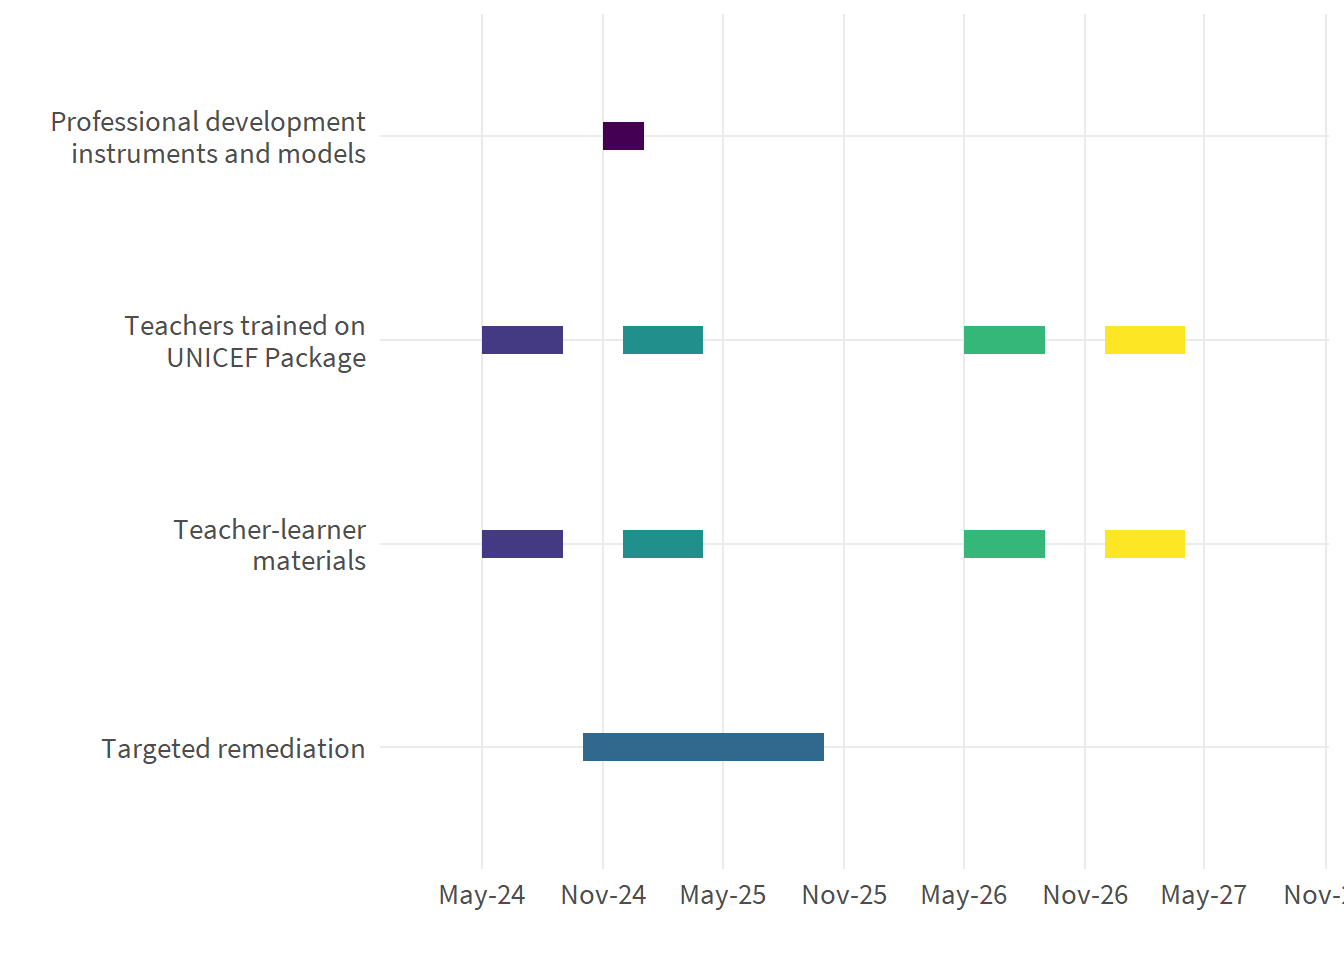
\includegraphics{Data-exploration_files/figure-pdf/unnamed-chunk-10-1.pdf}

This Gantt is more visually appealing, and still retains utility in
highlighting what activities occur and when. Note that we have
suppressed the legend created by the color aesthetic, but we could have
kept it in order to communicate additional information.

Additional resources:

\href{https://www.molecularecologist.com/2019/01/03/simple-gantt-charts-in-r-with-ggplot2-and-the-tidyverse/}{Simple
Gantt charts in R with ggplot2 \ldots{} and Microsoft Excel}

\href{https://plotly.com/ggplot2/gantt/}{Gantt charts using ggplott and
Plotly}

\href{https://www.appsilon.com/post/r-shiny-gantt-chart-planning-management}{R
Shiny Gantt Chart}

\href{https://www.statology.org/gantt-chart-r-ggplot2/}{How to Create a
Gantt Chart in R Using ggplot2}

Happy Gantting!

\chapter{Mapping}\label{mapping}

Much of our data is collected from surveys and has geographic
coordinates associated with a point of collection, a house, or a city,
etc. It can be useful to generate a map to get a sense of where the data
is coming from. Mapping is a part of MSI's exploratory data analysis
process and is also used in developing a sampling plan and in producing
high quality data vizualizations for clients. This section provides a
brief introduction into mapping in R.

The most commonly used packages to handle spatial data are \texttt{sf}
for vectors, \texttt{terra} for vectors and rasters, and \texttt{raster}
for rasters. To visualize the data, two frequently used packages are
\href{https://r-tmap.github.io/tmap/}{tmap} and
\href{https://ggplot2.tidyverse.org/}{ggplot2} packages.

To get started, we need to load our packages.

\begin{Shaded}
\begin{Highlighting}[]
\CommentTok{\#run this line first if you have never used these packages before}
\CommentTok{\#install.packages(c("tidyverse", "sf", "tmap", "readr", "here"))}

\FunctionTok{library}\NormalTok{(tidyverse) }\CommentTok{\#install the core tidyverse packages including ggplot2}
\FunctionTok{library}\NormalTok{(sf) }\CommentTok{\#provides tools to work with vector data }
\FunctionTok{library}\NormalTok{(tmap) }\CommentTok{\#for visualizing spatial data}
\FunctionTok{library}\NormalTok{(readr) }\CommentTok{\#functions for reading external datasets }
\FunctionTok{library}\NormalTok{(here) }\CommentTok{\#to better locate files not in working directory}
\FunctionTok{library}\NormalTok{(geodata) }\CommentTok{\#to download administrative boundaries}
\end{Highlighting}
\end{Shaded}

\section{Read in the data}\label{read-in-the-data}

\begin{Shaded}
\begin{Highlighting}[]
\CommentTok{\#It is a csv file so I use the read\_csv function and provide the file path}
\NormalTok{cities }\OtherTok{\textless{}{-}} \FunctionTok{read\_csv}\NormalTok{(here}\SpecialCharTok{::}\FunctionTok{here}\NormalTok{(}\StringTok{"../methods corner/Map demo/data/Madagascar\_Cities.csv"}\NormalTok{)}
\NormalTok{                   , }\AttributeTok{show\_col\_types =} \ConstantTok{FALSE}\NormalTok{)}

\CommentTok{\#Observe the first few rows of data}
\NormalTok{DT}\SpecialCharTok{::}\FunctionTok{datatable}\NormalTok{(}\FunctionTok{head}\NormalTok{(cities))}
\end{Highlighting}
\end{Shaded}

\begin{verbatim}
Google Chrome was not found. Try setting the `CHROMOTE_CHROME` environment variable to the executable of a Chromium-based browser, such as Google Chrome, Chromium or Brave.
\end{verbatim}

\includegraphics{Data-exploration_files/figure-pdf/cities-1.pdf}

Now, for the administrative boundaries. Each of these are being read in
using \texttt{gadm()} from the \texttt{geodata} package and then
converted to an sf object with the \texttt{st\_as\_sf()} function. In
the example, we download only the country boundary, but if we wanted
regions or departments, we would simply change the level argument inside
the \texttt{gadm()} function call to a 1 or a 2.

\section{Country boundary}\label{country-boundary}

\begin{Shaded}
\begin{Highlighting}[]
\CommentTok{\#This is only the country boundary. }
\NormalTok{mdg }\OtherTok{\textless{}{-}}\NormalTok{ geodata}\SpecialCharTok{::}\FunctionTok{gadm}\NormalTok{(}\AttributeTok{country =} \StringTok{"MDG"}
\NormalTok{                  , }\AttributeTok{level =} \DecValTok{0}
\NormalTok{                  , }\AttributeTok{path =} \FunctionTok{tempdir}\NormalTok{()) }\SpecialCharTok{|\textgreater{}}
  \FunctionTok{st\_as\_sf}\NormalTok{()}
\end{Highlighting}
\end{Shaded}

\section{Convert the cities to an sf
object}\label{convert-the-cities-to-an-sf-object}

Remember that the cities object is a standard .csv with longitude and
latitude columns, but it is not yet recognized as an sf object that has
geographic properties. Here is how to convert it to an sf object with a
single geometry column and a crs.

\begin{Shaded}
\begin{Highlighting}[]
\NormalTok{cities\_sf }\OtherTok{\textless{}{-}}\NormalTok{ cities }\SpecialCharTok{|\textgreater{}}
  \FunctionTok{st\_as\_sf}\NormalTok{(}\AttributeTok{coords =} \FunctionTok{c}\NormalTok{(}\StringTok{"Longitude"}\NormalTok{, }\StringTok{"Latitude"}\NormalTok{)}
\NormalTok{           , }\AttributeTok{crs =} \DecValTok{4326}\NormalTok{)}

\CommentTok{\#observe the first few rows of data}
\NormalTok{DT}\SpecialCharTok{::}\FunctionTok{datatable}\NormalTok{(}\FunctionTok{head}\NormalTok{(cities\_sf))}
\end{Highlighting}
\end{Shaded}

\includegraphics{Data-exploration_files/figure-pdf/convert-1.pdf}

\section{Make the map}\label{make-the-map}

The following code chunks and tabs walk through the process of making
and improving a map in both tmap and ggplot2. In the example, cities are
what we are plotting, but we could be plotting any variable of a
dataset.

\section{tmap}

\begin{Shaded}
\begin{Highlighting}[]
\FunctionTok{tmap\_mode}\NormalTok{(}\StringTok{"plot"}\NormalTok{) }\SpecialCharTok{+}
  \FunctionTok{tm\_shape}\NormalTok{(mdg) }\SpecialCharTok{+}
  \FunctionTok{tm\_polygons}\NormalTok{() }\SpecialCharTok{+} \CommentTok{\#for only the borders, use tm\_borders()}
  \FunctionTok{tm\_shape}\NormalTok{(cities\_sf) }\SpecialCharTok{+}
  \FunctionTok{tm\_dots}\NormalTok{(}\AttributeTok{size =}\NormalTok{ .}\DecValTok{25}\NormalTok{, }\AttributeTok{col =} \StringTok{"red"}\NormalTok{)}
\end{Highlighting}
\end{Shaded}

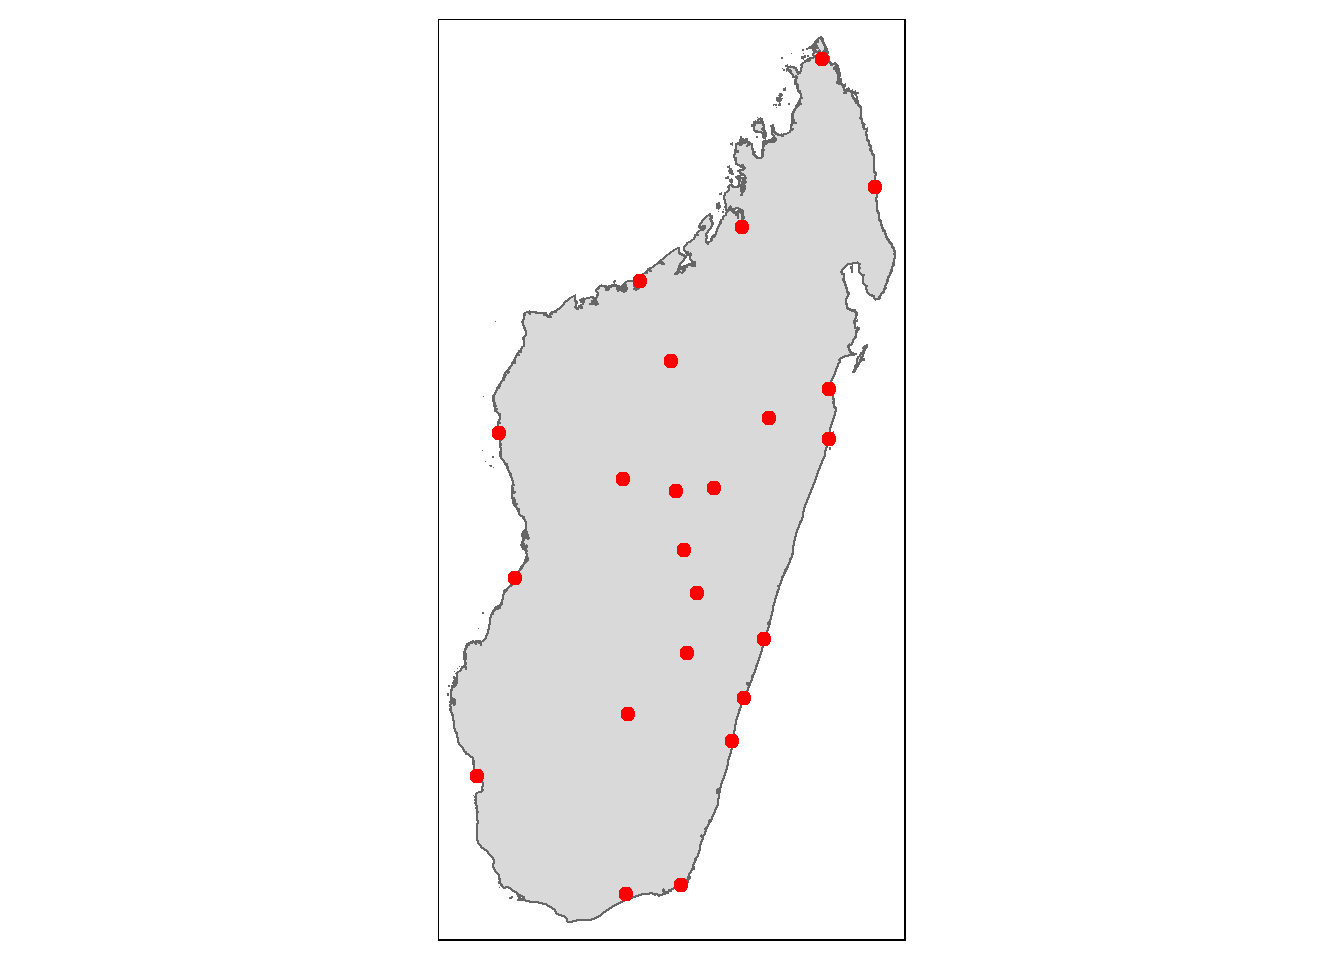
\includegraphics{Data-exploration_files/figure-pdf/tmap start-1.pdf}

\section{ggplot2}

\begin{Shaded}
\begin{Highlighting}[]
\NormalTok{ggplot2}\SpecialCharTok{::}\FunctionTok{ggplot}\NormalTok{(mdg) }\SpecialCharTok{+}
  \FunctionTok{geom\_sf}\NormalTok{() }\SpecialCharTok{+}
  \FunctionTok{geom\_sf}\NormalTok{(}\AttributeTok{data =}\NormalTok{ cities\_sf, }\AttributeTok{color =} \StringTok{"red"}\NormalTok{)}
\end{Highlighting}
\end{Shaded}

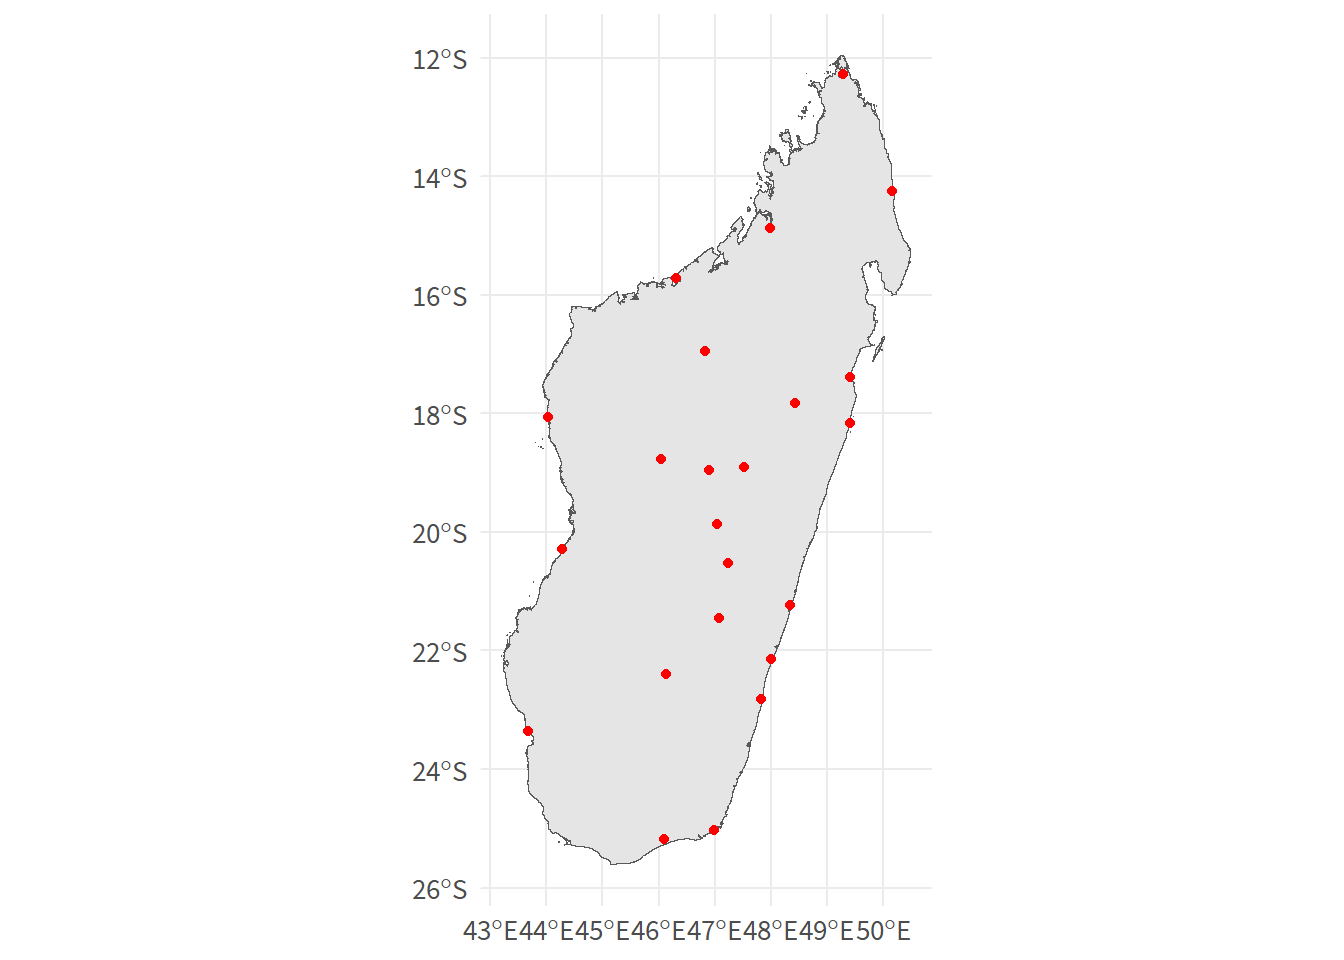
\includegraphics{Data-exploration_files/figure-pdf/ggplot2-1.pdf}

\section{Make the map better}\label{make-the-map-better}

\section{tmap}

\begin{Shaded}
\begin{Highlighting}[]
\CommentTok{\#the city names are long so we have to }
\CommentTok{\# make a bigger window to fit them. This isn\textquotesingle{}t part of the normal process}
\CommentTok{\#make an object with the current bounding box}
\NormalTok{bbox\_new }\OtherTok{\textless{}{-}} \FunctionTok{st\_bbox}\NormalTok{(mdg)}

\CommentTok{\#calculate the x and y ranges of the bbox}
\NormalTok{xrange }\OtherTok{\textless{}{-}}\NormalTok{ bbox\_new}\SpecialCharTok{$}\NormalTok{xmax }\SpecialCharTok{{-}}\NormalTok{ bbox\_new}\SpecialCharTok{$}\NormalTok{xmin }\CommentTok{\# range of x values}
\NormalTok{yrange }\OtherTok{\textless{}{-}}\NormalTok{ bbox\_new}\SpecialCharTok{$}\NormalTok{ymax }\SpecialCharTok{{-}}\NormalTok{ bbox\_new}\SpecialCharTok{$}\NormalTok{ymin }\CommentTok{\# range of y values}

\CommentTok{\#provide the new values for the 4 corners of the bbox}
\NormalTok{  bbox\_new[}\DecValTok{1}\NormalTok{] }\OtherTok{\textless{}{-}}\NormalTok{ bbox\_new[}\DecValTok{1}\NormalTok{] }\SpecialCharTok{{-}}\NormalTok{ (}\FloatTok{0.7} \SpecialCharTok{*}\NormalTok{ xrange) }\CommentTok{\# xmin {-} left}
\NormalTok{  bbox\_new[}\DecValTok{3}\NormalTok{] }\OtherTok{\textless{}{-}}\NormalTok{ bbox\_new[}\DecValTok{3}\NormalTok{] }\SpecialCharTok{+}\NormalTok{ (}\FloatTok{0.75} \SpecialCharTok{*}\NormalTok{ xrange) }\CommentTok{\# xmax {-} right}
\NormalTok{  bbox\_new[}\DecValTok{2}\NormalTok{] }\OtherTok{\textless{}{-}}\NormalTok{ bbox\_new[}\DecValTok{2}\NormalTok{] }\SpecialCharTok{{-}}\NormalTok{ (}\FloatTok{0.1} \SpecialCharTok{*}\NormalTok{ yrange) }\CommentTok{\# ymin {-} bottom}
\NormalTok{  bbox\_new[}\DecValTok{4}\NormalTok{] }\OtherTok{\textless{}{-}}\NormalTok{ bbox\_new[}\DecValTok{4}\NormalTok{] }\SpecialCharTok{+}\NormalTok{ (}\FloatTok{0.1} \SpecialCharTok{*}\NormalTok{ yrange) }\CommentTok{\# ymax {-} top}

\CommentTok{\#convert the bbox to a sf collection (sfc)}
\NormalTok{bbox\_new }\OtherTok{\textless{}{-}}\NormalTok{ bbox\_new }\SpecialCharTok{|\textgreater{}}  \CommentTok{\# take the bounding box ...}
  \FunctionTok{st\_as\_sfc}\NormalTok{() }\CommentTok{\# ... and make it a sf polygon}

\CommentTok{\#now plot the map}
\FunctionTok{tmap\_mode}\NormalTok{(}\StringTok{"plot"}\NormalTok{) }\SpecialCharTok{+}
  \FunctionTok{tm\_shape}\NormalTok{(mdg, }\AttributeTok{bbox =}\NormalTok{ bbox\_new) }\SpecialCharTok{+}
  \FunctionTok{tm\_polygons}\NormalTok{() }\SpecialCharTok{+}
  \FunctionTok{tm\_shape}\NormalTok{(cities\_sf) }\SpecialCharTok{+}
  \FunctionTok{tm\_dots}\NormalTok{(}\AttributeTok{size =}\NormalTok{ .}\DecValTok{25}\NormalTok{, }\AttributeTok{col =} \StringTok{"red"}\NormalTok{) }\SpecialCharTok{+}
  \FunctionTok{tm\_text}\NormalTok{(}\AttributeTok{text =} \StringTok{"Name"}\NormalTok{, }\AttributeTok{auto.placement =}\NormalTok{ T) }\SpecialCharTok{+}
  \FunctionTok{tm\_layout}\NormalTok{(}\AttributeTok{title =} \StringTok{"Main Cities of}\SpecialCharTok{\textbackslash{}n}\StringTok{Madagascar"}\NormalTok{)}
\end{Highlighting}
\end{Shaded}

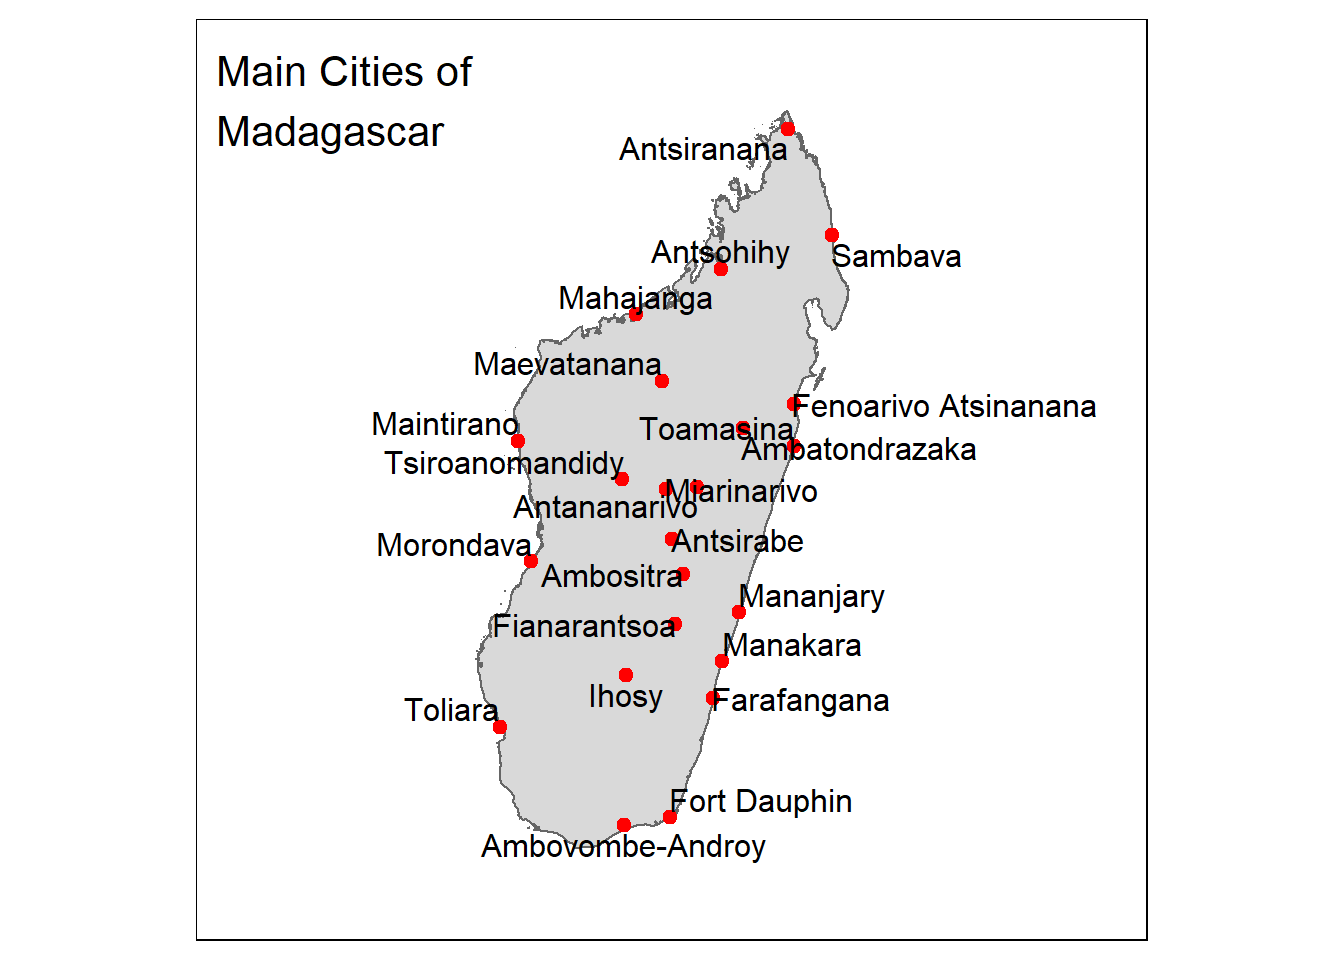
\includegraphics{Data-exploration_files/figure-pdf/tmap middle-1.pdf}

\section{ggplot2}

\begin{Shaded}
\begin{Highlighting}[]
\CommentTok{\#the city names are long so we have to }
\CommentTok{\# make a bigger window to fit them. This isn\textquotesingle{}t part of the normal process}
\CommentTok{\#make an object with the current bounding box}
\NormalTok{bbox\_new }\OtherTok{\textless{}{-}} \FunctionTok{st\_bbox}\NormalTok{(mdg)}

\CommentTok{\#calculate the x and y ranges of the bbox}
\NormalTok{xrange }\OtherTok{\textless{}{-}}\NormalTok{ bbox\_new}\SpecialCharTok{$}\NormalTok{xmax }\SpecialCharTok{{-}}\NormalTok{ bbox\_new}\SpecialCharTok{$}\NormalTok{xmin }\CommentTok{\# range of x values}
\NormalTok{yrange }\OtherTok{\textless{}{-}}\NormalTok{ bbox\_new}\SpecialCharTok{$}\NormalTok{ymax }\SpecialCharTok{{-}}\NormalTok{ bbox\_new}\SpecialCharTok{$}\NormalTok{ymin }\CommentTok{\# range of y values}

\CommentTok{\#provide the new values for the 4 corners of the bbox}
\NormalTok{  bbox\_new[}\DecValTok{1}\NormalTok{] }\OtherTok{\textless{}{-}}\NormalTok{ bbox\_new[}\DecValTok{1}\NormalTok{] }\SpecialCharTok{{-}}\NormalTok{ (}\FloatTok{0.5} \SpecialCharTok{*}\NormalTok{ xrange) }\CommentTok{\# xmin {-} left}
\NormalTok{  bbox\_new[}\DecValTok{3}\NormalTok{] }\OtherTok{\textless{}{-}}\NormalTok{ bbox\_new[}\DecValTok{3}\NormalTok{] }\SpecialCharTok{+}\NormalTok{ (}\FloatTok{0.5} \SpecialCharTok{*}\NormalTok{ xrange) }\CommentTok{\# xmax {-} right}
\NormalTok{  bbox\_new[}\DecValTok{2}\NormalTok{] }\OtherTok{\textless{}{-}}\NormalTok{ bbox\_new[}\DecValTok{2}\NormalTok{] }\SpecialCharTok{{-}}\NormalTok{ (}\FloatTok{0.1} \SpecialCharTok{*}\NormalTok{ yrange) }\CommentTok{\# ymin {-} bottom}
\NormalTok{  bbox\_new[}\DecValTok{4}\NormalTok{] }\OtherTok{\textless{}{-}}\NormalTok{ bbox\_new[}\DecValTok{4}\NormalTok{] }\SpecialCharTok{+}\NormalTok{ (}\FloatTok{0.1} \SpecialCharTok{*}\NormalTok{ yrange) }\CommentTok{\# ymax {-} top}

\CommentTok{\#convert the bbox to a sf collection (sfc)}
\NormalTok{bbox\_new }\OtherTok{\textless{}{-}}\NormalTok{ bbox\_new }\SpecialCharTok{|\textgreater{}}  \CommentTok{\# take the bounding box}
  \FunctionTok{st\_as\_sfc}\NormalTok{() }\CommentTok{\# ... and make it a sf polygon}


\NormalTok{ggplot2}\SpecialCharTok{::}\FunctionTok{ggplot}\NormalTok{() }\SpecialCharTok{+}
  \FunctionTok{geom\_sf}\NormalTok{(}\AttributeTok{data =}\NormalTok{ mdg) }\SpecialCharTok{+}
  \FunctionTok{geom\_sf}\NormalTok{(}\AttributeTok{data =}\NormalTok{ cities\_sf, }\AttributeTok{color =} \StringTok{"red"}\NormalTok{) }\SpecialCharTok{+}
\NormalTok{  ggrepel}\SpecialCharTok{::}\FunctionTok{geom\_text\_repel}\NormalTok{(}\AttributeTok{data =}\NormalTok{ cities\_sf}
\NormalTok{               , }\FunctionTok{aes}\NormalTok{(}\AttributeTok{label =}\NormalTok{ Name}
\NormalTok{                     , }\AttributeTok{geometry =}\NormalTok{ geometry)}
\NormalTok{               , }\AttributeTok{stat =} \StringTok{"sf\_coordinates"}
\NormalTok{               , }\AttributeTok{min.segment.length =} \DecValTok{0}\NormalTok{) }\SpecialCharTok{+}
  \FunctionTok{coord\_sf}\NormalTok{(}\AttributeTok{xlim =} \FunctionTok{st\_coordinates}\NormalTok{(bbox\_new)[}\FunctionTok{c}\NormalTok{(}\DecValTok{1}\NormalTok{,}\DecValTok{2}\NormalTok{),}\DecValTok{1}\NormalTok{], }\CommentTok{\# min \& max of x values}
           \AttributeTok{ylim =} \FunctionTok{st\_coordinates}\NormalTok{(bbox\_new)[}\FunctionTok{c}\NormalTok{(}\DecValTok{2}\NormalTok{,}\DecValTok{3}\NormalTok{),}\DecValTok{2}\NormalTok{]) }\SpecialCharTok{+} \CommentTok{\# min \& max of y values +}
  \FunctionTok{labs}\NormalTok{(}\AttributeTok{title =} \StringTok{"Main Cities of}\SpecialCharTok{\textbackslash{}n}\StringTok{Madagascar"}\NormalTok{) }\SpecialCharTok{+}
  \FunctionTok{theme\_void}\NormalTok{()}
\end{Highlighting}
\end{Shaded}

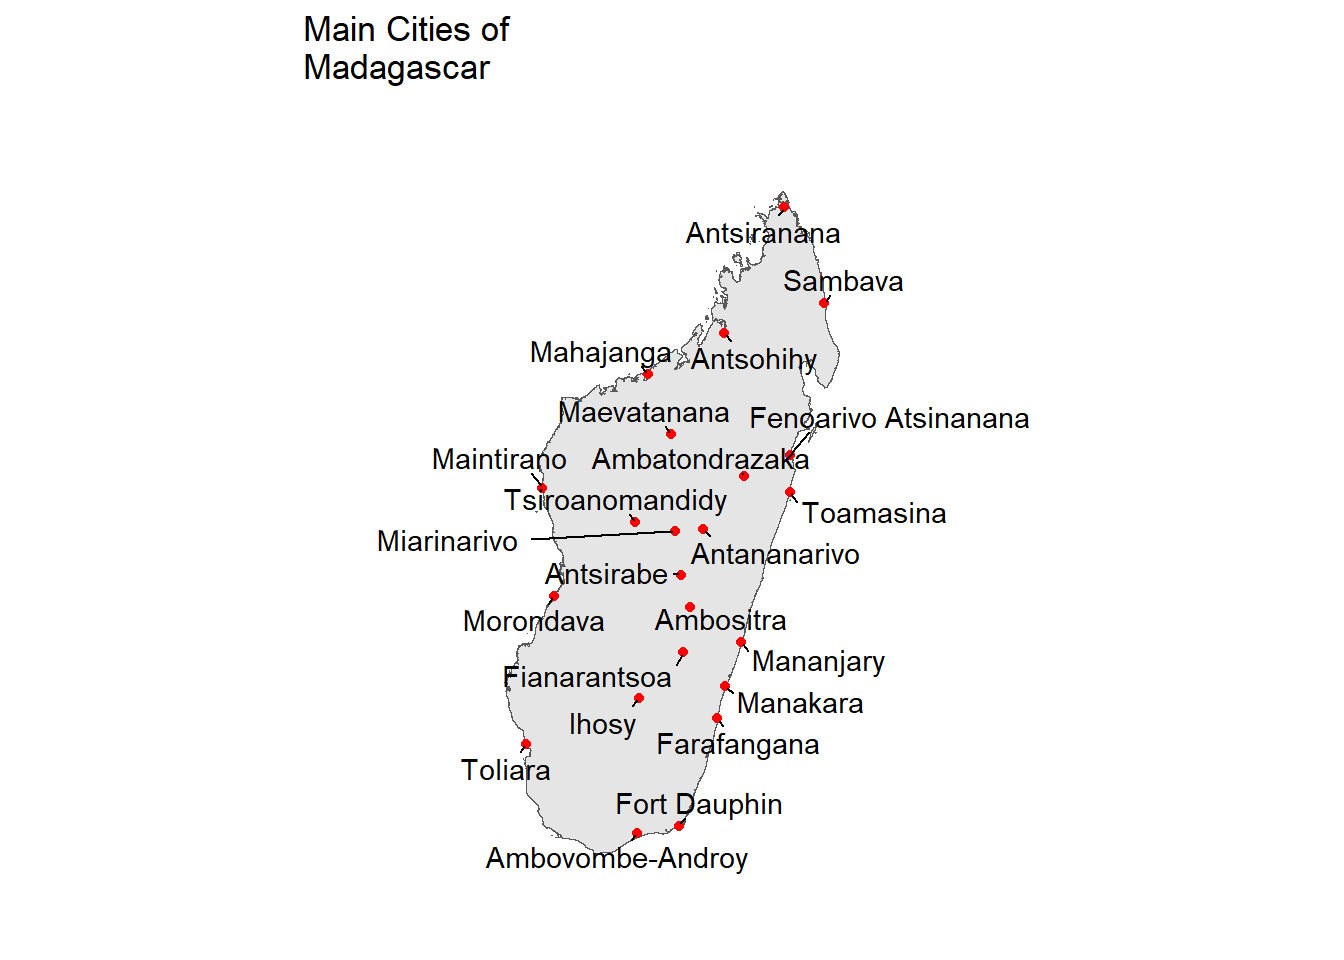
\includegraphics{Data-exploration_files/figure-pdf/ggplot middle-1.pdf}

\section{Final touches}\label{final-touches}

Now that we have a map with cities plotted (we achieved our goal!), we
will add a few finishing touches and set the size of the city points to
the \texttt{population} variable in the original dataset.

Additionally, tmap provides a simple interface to go from a static map
to an interative map simply by changing \texttt{tmap\_mode("plot")} to
\texttt{tmap\_mode("view")}.

\section{tmap}

\begin{Shaded}
\begin{Highlighting}[]
\CommentTok{\#the city names are long so we have to }
\CommentTok{\# make a bigger window to fit them. This isn\textquotesingle{}t part of the normal process}
\CommentTok{\#make an object with the current bounding box}
\NormalTok{bbox\_new }\OtherTok{\textless{}{-}} \FunctionTok{st\_bbox}\NormalTok{(mdg)}

\CommentTok{\#calculate the x and y ranges of the bbox}
\NormalTok{xrange }\OtherTok{\textless{}{-}}\NormalTok{ bbox\_new}\SpecialCharTok{$}\NormalTok{xmax }\SpecialCharTok{{-}}\NormalTok{ bbox\_new}\SpecialCharTok{$}\NormalTok{xmin }\CommentTok{\# range of x values}
\NormalTok{yrange }\OtherTok{\textless{}{-}}\NormalTok{ bbox\_new}\SpecialCharTok{$}\NormalTok{ymax }\SpecialCharTok{{-}}\NormalTok{ bbox\_new}\SpecialCharTok{$}\NormalTok{ymin }\CommentTok{\# range of y values}

\CommentTok{\#provide the new values for the 4 corners of the bbox}
\NormalTok{  bbox\_new[}\DecValTok{1}\NormalTok{] }\OtherTok{\textless{}{-}}\NormalTok{ bbox\_new[}\DecValTok{1}\NormalTok{] }\SpecialCharTok{{-}}\NormalTok{ (}\FloatTok{0.7} \SpecialCharTok{*}\NormalTok{ xrange) }\CommentTok{\# xmin {-} left}
\NormalTok{  bbox\_new[}\DecValTok{3}\NormalTok{] }\OtherTok{\textless{}{-}}\NormalTok{ bbox\_new[}\DecValTok{3}\NormalTok{] }\SpecialCharTok{+}\NormalTok{ (}\FloatTok{0.75} \SpecialCharTok{*}\NormalTok{ xrange) }\CommentTok{\# xmax {-} right}
\NormalTok{  bbox\_new[}\DecValTok{2}\NormalTok{] }\OtherTok{\textless{}{-}}\NormalTok{ bbox\_new[}\DecValTok{2}\NormalTok{] }\SpecialCharTok{{-}}\NormalTok{ (}\FloatTok{0.1} \SpecialCharTok{*}\NormalTok{ yrange) }\CommentTok{\# ymin {-} bottom}
\NormalTok{  bbox\_new[}\DecValTok{4}\NormalTok{] }\OtherTok{\textless{}{-}}\NormalTok{ bbox\_new[}\DecValTok{4}\NormalTok{] }\SpecialCharTok{+}\NormalTok{ (}\FloatTok{0.1} \SpecialCharTok{*}\NormalTok{ yrange) }\CommentTok{\# ymax {-} top}

\CommentTok{\#convert the bbox to a sf collection (sfc)}
\NormalTok{bbox\_new }\OtherTok{\textless{}{-}}\NormalTok{ bbox\_new }\SpecialCharTok{|\textgreater{}}  \CommentTok{\# take the bounding box ...}
  \FunctionTok{st\_as\_sfc}\NormalTok{() }\CommentTok{\# ... and make it a sf polygon}
\FunctionTok{tmap\_mode}\NormalTok{(}\StringTok{"plot"}\NormalTok{) }\SpecialCharTok{+}
  \FunctionTok{tm\_shape}\NormalTok{(mdg, }\AttributeTok{bbox =}\NormalTok{ bbox\_new) }\SpecialCharTok{+}
  \FunctionTok{tm\_polygons}\NormalTok{() }\SpecialCharTok{+}
  \FunctionTok{tm\_shape}\NormalTok{(cities\_sf) }\SpecialCharTok{+}
  \FunctionTok{tm\_dots}\NormalTok{(}\AttributeTok{size =} \StringTok{"Population"}\NormalTok{, }\AttributeTok{col =} \StringTok{"red"}
\NormalTok{          , }\AttributeTok{legend.size.is.portrait =} \ConstantTok{TRUE}\NormalTok{) }\SpecialCharTok{+}
  \FunctionTok{tm\_text}\NormalTok{(}\AttributeTok{text =} \StringTok{"Name"}\NormalTok{, }\AttributeTok{auto.placement =}\NormalTok{ T}
\NormalTok{          , }\AttributeTok{along.lines =}\NormalTok{ T) }\SpecialCharTok{+}
  \FunctionTok{tm\_scale\_bar}\NormalTok{(}\AttributeTok{position =} \FunctionTok{c}\NormalTok{(}\StringTok{"left"}\NormalTok{, }\StringTok{"bottom"}\NormalTok{), }\AttributeTok{width =} \FloatTok{0.15}\NormalTok{) }\SpecialCharTok{+}
  \FunctionTok{tm\_compass}\NormalTok{(}\AttributeTok{type =} \StringTok{"4star"}
\NormalTok{             , }\AttributeTok{position =} \FunctionTok{c}\NormalTok{(}\StringTok{"right"}\NormalTok{, }\StringTok{"bottom"}\NormalTok{)}
\NormalTok{             , }\AttributeTok{size =} \DecValTok{2}\NormalTok{) }\SpecialCharTok{+}
  \FunctionTok{tm\_layout}\NormalTok{(}\AttributeTok{main.title =} \StringTok{"Main Cities of Madagascar"}\NormalTok{                         , }\AttributeTok{legend.outside =} \ConstantTok{TRUE}\NormalTok{)}
\end{Highlighting}
\end{Shaded}

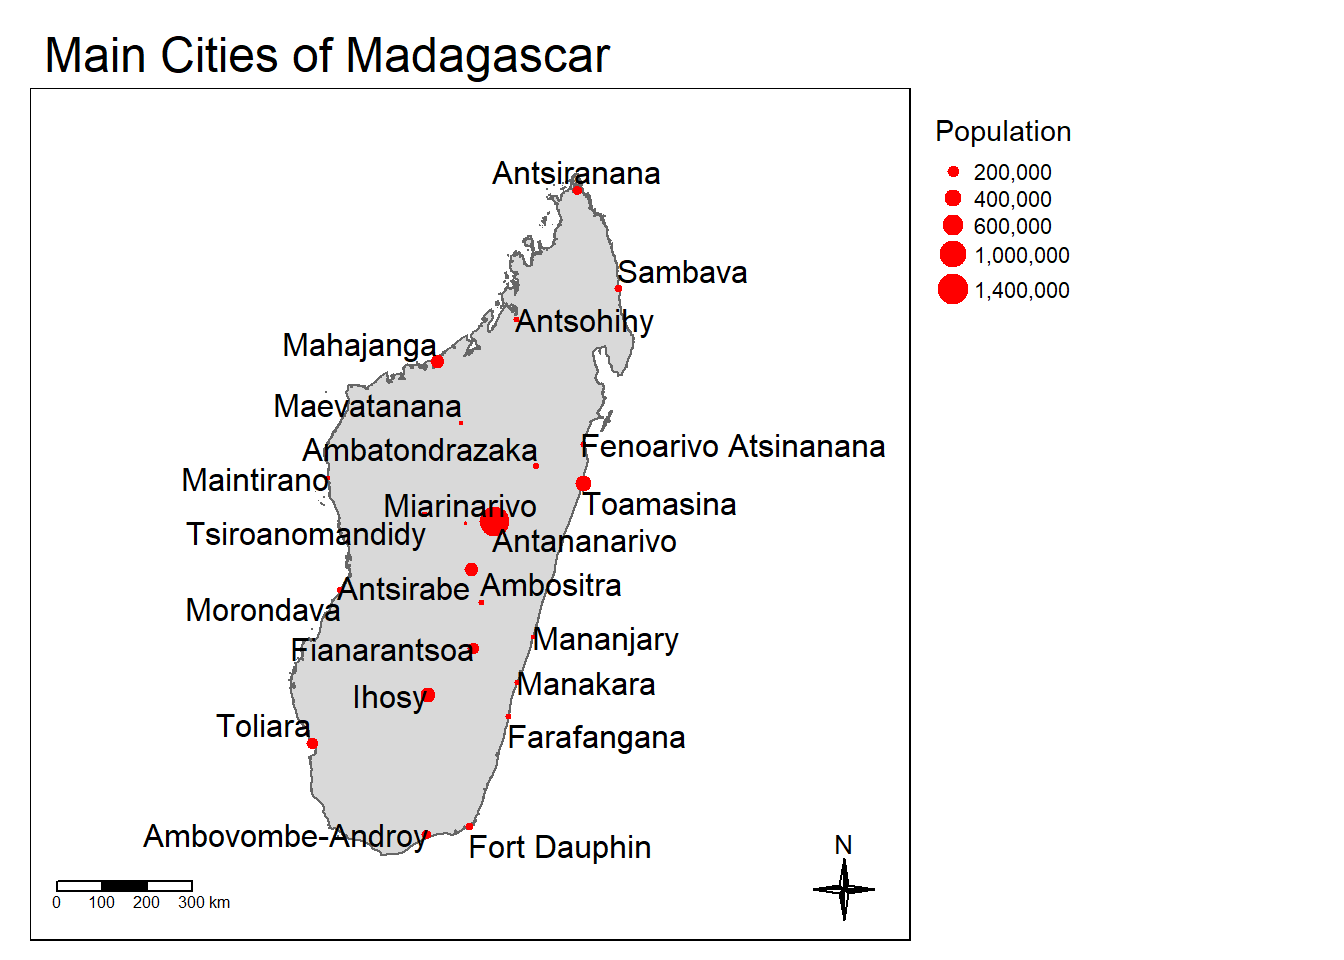
\includegraphics{Data-exploration_files/figure-pdf/tmap final-1.pdf}

\section{ggplot2}

\begin{Shaded}
\begin{Highlighting}[]
\NormalTok{ggplot2}\SpecialCharTok{::}\FunctionTok{ggplot}\NormalTok{() }\SpecialCharTok{+}
  \FunctionTok{geom\_sf}\NormalTok{(}\AttributeTok{data =}\NormalTok{ mdg) }\SpecialCharTok{+}
  \FunctionTok{geom\_sf}\NormalTok{(}\AttributeTok{data =}\NormalTok{ cities\_sf, }\FunctionTok{aes}\NormalTok{(}\AttributeTok{size =}\NormalTok{ Population)}
\NormalTok{          , }\AttributeTok{color =} \StringTok{"red"}\NormalTok{) }\SpecialCharTok{+}
\NormalTok{  ggrepel}\SpecialCharTok{::}\FunctionTok{geom\_text\_repel}\NormalTok{(}\AttributeTok{data =}\NormalTok{ cities\_sf}
\NormalTok{               , }\FunctionTok{aes}\NormalTok{(}\AttributeTok{label =}\NormalTok{ Name}
\NormalTok{                     , }\AttributeTok{geometry =}\NormalTok{ geometry)}
\NormalTok{               , }\AttributeTok{stat =} \StringTok{"sf\_coordinates"}
\NormalTok{               , }\AttributeTok{min.segment.length =} \DecValTok{0}\NormalTok{) }\SpecialCharTok{+}
  \FunctionTok{coord\_sf}\NormalTok{(}\AttributeTok{xlim =} \FunctionTok{st\_coordinates}\NormalTok{(bbox\_new)[}\FunctionTok{c}\NormalTok{(}\DecValTok{1}\NormalTok{,}\DecValTok{2}\NormalTok{),}\DecValTok{1}\NormalTok{], }\CommentTok{\# min \& max of x values}
           \AttributeTok{ylim =} \FunctionTok{st\_coordinates}\NormalTok{(bbox\_new)[}\FunctionTok{c}\NormalTok{(}\DecValTok{2}\NormalTok{,}\DecValTok{3}\NormalTok{),}\DecValTok{2}\NormalTok{]) }\SpecialCharTok{+} \CommentTok{\# min \& max of y values +}
\NormalTok{  ggspatial}\SpecialCharTok{::}\FunctionTok{annotation\_scale}\NormalTok{(}\AttributeTok{location =} \StringTok{"bl"}\NormalTok{) }\SpecialCharTok{+}
\NormalTok{  ggspatial}\SpecialCharTok{::}\FunctionTok{annotation\_north\_arrow}\NormalTok{(}\AttributeTok{location =} \StringTok{"br"}
\NormalTok{                                    , }\AttributeTok{which\_north =} \StringTok{"true"}
\NormalTok{                                    , }\AttributeTok{size =} \DecValTok{1}\NormalTok{)}\SpecialCharTok{+}
  \FunctionTok{labs}\NormalTok{(}\AttributeTok{title =} \StringTok{"Main Cities of Madagascar"}\NormalTok{) }\SpecialCharTok{+}
  \FunctionTok{theme\_void}\NormalTok{()}
\end{Highlighting}
\end{Shaded}

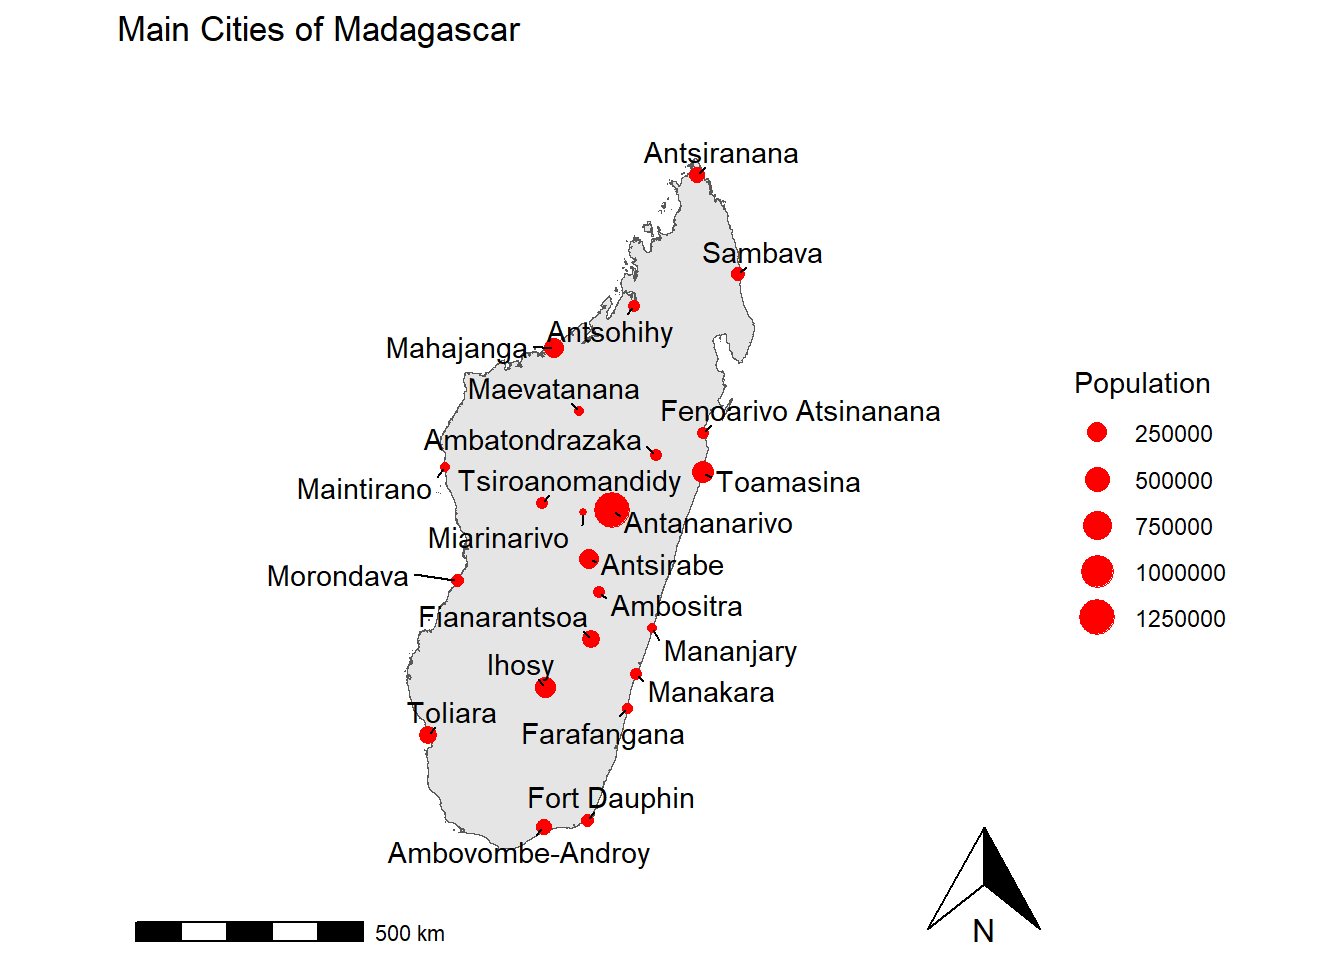
\includegraphics{Data-exploration_files/figure-pdf/ggplot final-1.pdf}

\section{tmap interactive}

\begin{Shaded}
\begin{Highlighting}[]
\FunctionTok{tmap\_mode}\NormalTok{(}\StringTok{"view"}\NormalTok{) }\SpecialCharTok{+}
  \FunctionTok{tm\_shape}\NormalTok{(mdg) }\SpecialCharTok{+}
  \FunctionTok{tm\_borders}\NormalTok{() }\SpecialCharTok{+}
  \FunctionTok{tm\_shape}\NormalTok{(cities\_sf) }\SpecialCharTok{+}
  \FunctionTok{tm\_dots}\NormalTok{(}\AttributeTok{size =} \StringTok{"Population"}\NormalTok{, }\AttributeTok{col =} \StringTok{"red"}
\NormalTok{          , }\AttributeTok{legend.size.is.portrait =} \ConstantTok{TRUE}\NormalTok{) }\SpecialCharTok{+}
  \FunctionTok{tm\_text}\NormalTok{(}\AttributeTok{text =} \StringTok{"Name"}\NormalTok{, }\AttributeTok{auto.placement =}\NormalTok{ T}
\NormalTok{          , }\AttributeTok{along.lines =}\NormalTok{ T) }\SpecialCharTok{+}
  \FunctionTok{tm\_scale\_bar}\NormalTok{(}\AttributeTok{position =} \FunctionTok{c}\NormalTok{(}\StringTok{"left"}\NormalTok{, }\StringTok{"bottom"}\NormalTok{), }\AttributeTok{width =} \FloatTok{0.15}\NormalTok{) }\SpecialCharTok{+}
  \FunctionTok{tm\_compass}\NormalTok{(}\AttributeTok{type =} \StringTok{"4star"}
\NormalTok{             , }\AttributeTok{position =} \FunctionTok{c}\NormalTok{(}\StringTok{"right"}\NormalTok{, }\StringTok{"bottom"}\NormalTok{)}
\NormalTok{             , }\AttributeTok{size =} \DecValTok{2}\NormalTok{) }\SpecialCharTok{+}
  \FunctionTok{tm\_layout}\NormalTok{(}\AttributeTok{main.title =} \StringTok{"Main Cities of Madagascar"}\NormalTok{                         , }\AttributeTok{legend.outside =} \ConstantTok{TRUE}\NormalTok{)}
\end{Highlighting}
\end{Shaded}

\includegraphics{Data-exploration_files/figure-pdf/tmap interactive-1.pdf}

\section{Additional Resources}\label{additional-resources}

For those interested in mapping in R (or QGIS) there are many free
resources available online. A great starting point for R is the online
text book, \href{https://r.geocompx.org/}{Geocomputation with R}. If you
would rather learn more in Python,
\href{https://py.geocompx.org/}{Geocomputation with Python} is a great
resource.

\chapter{Data modeling}\label{data-modeling}

\chapter{Generating client
deliverables}\label{generating-client-deliverables}

\part{Reporting}

\chapter{Reports}\label{reports}

\chapter{Presentations}\label{presentations}

\chapter{Dashboards}\label{dashboards}

\part{Annexes}

\chapter*{References}\label{references}
\addcontentsline{toc}{chapter}{References}

\markboth{References}{References}

\phantomsection\label{refs}
\begin{CSLReferences}{0}{1}
\end{CSLReferences}



\end{document}
